\documentclass[12pt,a4paper,twoside,french]{book}
\RequirePackage[l2tabu, orthodox]{nag}
\usepackage{cmap}
\usepackage{lmodern}  
\usepackage[utf8]{inputenc}
\usepackage[T1]{fontenc}
\usepackage{microtype}
\usepackage{cleveref} %GEEENIAAAAL!!!
\usepackage[top=2.05cm,bottom=1.1cm,left=0.5cm,right=5.5cm,marginparsep=0.8cm,marginparwidth=4.4cm]{geometry}
\usepackage{booktabs}
%\usepackage{vmargin}
\usepackage{media9}
\usepackage{layout}
\usepackage[pdftex]{graphicx}
\usepackage[svgnames,x11names]{xcolor}
\usepackage{titlesec}
\usepackage{setspace}
\usepackage{pstricks}% for pdflatex --shell-escape
\usepackage{pst-pdf}
\usepackage{pst-eucl}	
\usepackage{pgf}
\usepackage{soul}
\usepackage[outline]{contour}
\usepackage{eqnarray}
\usepackage{tikz}
\usetikzlibrary{shapes,positioning}
\usepackage{lscape}
\usepackage{url}
\usepackage[subfigure]{tocloft}
\setlength{\cftfignumwidth}{3em}
\usepackage{fancyhdr}
\usepackage{blindtext}
\usepackage{ae}
\usepackage{wrapfig}
\usepackage{framed}
\usepackage{colortbl}
\usepackage{amssymb,mathrsfs}
\usepackage{makeidx}
\usepackage{lettrine}
\usepackage{fancybox}
\usepackage{subfigure}
\usepackage{multirow}
\usepackage{multicol}
\usepackage{graphicx}
\usepackage{eso-pic}
\usepackage{lipsum}
%\usepackage{subcaption}
\usepackage[Bjornstrup]{fncychap}
\usepackage{hyperref}
\usepackage[french]{minitoc}
\hypersetup{colorlinks=true,breaklinks=true,bookmarksopen=true,urlcolor=black,linkcolor=gray}                                                    
\setlength{\fboxsep}{0mm}
\renewcommand {\mtctitle} {}
\usepackage{etex}
\usepackage{ifthen}
\usepackage{marginnote}
\usepackage{lipsum}
\usepackage{chngpage}
\usepackage{pdfcomment}
\usepackage{feynmp}
\usepackage{pgfplots}
\usepackage{wallpaper}
\pgfplotsset{width=10cm,compat=1.9}
\renewcommand{\baselinestretch}{1}

\newcommand{\ColorSection}[1]{%
    \colorbox{black!65}{\parbox[c][1.5em][c]{\dimexpr\textwidth-2\fboxsep}
    {\hspace{0.2cm}\textcolor{white}{\thesection\ #1}\hspace*{0.5cm}}}}
\newcommand{\ColorSectionStarred}[1]{%
    \colorbox{black!65}{\parbox[c][1.5em][c]{\dimexpr\textwidth-2\fboxsep}
    {#1}}}
\titlespacing*{\section}{0pt}{\baselineskip}{\baselineskip}

\titleformat{\section}
    {\rmfamily\large\raggedright}                                                
    {}{0pt}{\ColorSection}     

\titleformat{name=\section,numberless}
    {\rmfamily\large\raggedright}                                                
    {}{0pt}{\ColorSectionStarred}       

\makeatletter
\renewcommand\chapter{\if@openright\cleardoublepage\else\clearpage\fi
                    \thispagestyle{empty}%
                  \global\@topnum\z@
                   \@afterindentfalse
                    \secdef\@chapter\@schapter}
\renewcommand\part{\if@openright\cleardoublepage\else\clearpage\fi
                    \thispagestyle{empty}%
                    \global\@topnum\z@
                    \@afterindentfalse
                    \secdef\@part\@spart}
\def\cleardoublepage{\clearpage\if@twoside \ifodd\c@page\else
\hbox{}\thispagestyle{empty}\newpage\if@twocolumn\hbox{}\newpage\fi\fi\fi}
\makeatother
\newenvironment{Figure}
  {\par\medskip\noindent\minipage{\linewidth}}
  {\endminipage\par\medskip}


\setlength{\mtcindent}{0cm}
\mtcsetdepth{minitoc}{4}
\usepackage{babel}
\usepackage{caption}
\usepackage{listings}
\let\oldfootnotesize\footnotesize
\renewcommand*{\footnotesize}{\oldfootnotesize\fontsize{5}{7}}

\captionsetup{
  justification=raggedright,
  labelfont={color=gray,bf,small},
  font=footnotesize}

\newcommand{\ligne}{\color{gray}{\rule{\linewidth}{5pt}}
\vspace{0.2cm}
\color{black}}

\makeatletter
\newcommand\At@Page@Upper@Right[1]{%
  \put(\LenToUnit{\paperwidth},\LenToUnit{\paperheight}){#1}%
}
\newcommand\AtPageLowerRight[1]{\At@Page@Upper@Right{%
  \put(0,\LenToUnit{-\paperheight}){\llap{#1}}}}
\makeatother

\renewcommand{\contentsname}{Table des matières}
\renewcommand{\thechapter}{\arabic{chapter}}
\renewcommand{\thesection}{\arabic{section}}
\renewcommand{\thesubsection}{\thesection.\arabic{subsection}}
\renewcommand{\thesubsubsection}{\thesection.\thesubsection.{subsubsection}}



%% Command to hold chapter illustration image
\newcommand\chapterillustration{}
\titlespacing*{\chapter}{0pt}{0pt}{135mm}





%%%%********************************************************************
% fancy quotes
\definecolor{quotemark}{gray}{0.7}
\makeatletter
\def\fquote{%
    \@ifnextchar[{\fquote@i}{\fquote@i[]}%]
}%
\def\fquote@i[#1]{%
    \def\tempa{#1}%
    \@ifnextchar[{\fquote@ii}{\fquote@ii[]}%]
}%
\def\fquote@ii[#1]{%
    \def\tempb{#1}%
    \@ifnextchar[{\fquote@iii}{\fquote@iii[]}%]
}%
\def\fquote@iii[#1]{%
    \def\tempc{#1}%
    \@ifnextchar[{\fquote@iiii}{\fquote@iiii[]}%]
}%
\def\fquote@iiii[#1]{%
    \def\tempd{#1}%
    \vspace{1em}%
    \noindent%
    \begin{list}{}
    {%
    		\setlength{\leftmargin}{0.1\textwidth}%
      \setlength{\rightmargin}{0.1\textwidth}%
    }%
    \item[]%
    \begin{picture}(0,0)%
    \put(\tempd,-15){\makebox(0,0){\scalebox{3}{\textcolor{quotemark}{``}}}}%
    \end{picture}%
    \begingroup\itshape
 }%
 %%%%********************************************************************
 \def\endfquote
 {%
 	\endgroup\par%
 	\makebox[0pt][l]{%
 	\hspace{0.8\textwidth}%
 	\begin{picture}(0,0)(0,0)%
 	\put(15,8){\makebox(0,0){\scalebox{3}{\color{quotemark}''}}}%
 	\end{picture}}%
 	\ifx\tempa\empty%
 	\else%
  \ifx\tempb\empty%
  \hfill\mbox{}\hfill\tempa%
  \else%
  \ifx\tempc\empty%
  \hfill\mbox{}\hfill\tempa,\ \emph{\tempb}%
  \else%
  \hfill\mbox{}\hfill\tempa,\ \emph{\tempb},\ \tempc%
  \fi\fi\par%
  \vspace{0.5em}%
 	\end{list}%
 }%
 \makeatother
 %%%%********************************************************************


\setcounter{tocdepth}{4}
\makeindex

\renewcommand{\LettrineFontHook}{\color{gray}}

\newcommand{\dd}{\mathrm{d}}

\newcommand{\pa}[2]{\frac{\partial #1}{\partial #2}}
\newcommand{\de}[2]{\frac{\dd #1}{\dd #2}}

\newcommand{\image}[4]{\begin{figure}[!ht]

\centering

\includegraphics[scale=#2]{#1}
\caption{#3} 
\label{#4}
\end{figure}}
\usetikzlibrary{shapes,calc}  

\usepackage{yfonts}

\newcommand{\lettrines}[2]{\lettrine[lines=2, slope= -0.5em, lhang=0.25, loversize=0.25]{#1}{\small #2}}







%%%%%%%%%%%%%%%%%%%%%%%%%%%%%%%%%
% Page de couverture %%%%%%%%%%%%%%%%%%%%%%
%%%%%%%%%%%%%%%%%%%%%%%%%%%%%%%%%
\makeatletter
\def\clap#1{\hbox to 0pt{\hss #1\hss}}%
\def\ligne#1{
  \hbox to \hsize{
    \vbox{\centering #1}}}

\def\haut#1#2#3{
  \hbox to \hsize{
    \rlap{\vtop{\raggedright #1}}
    \hss
    \clap{\vtop{\centering #2}}
    \hss
    \llap{\vtop{\raggedleft #3}}}}

\def\bas#1#2#3{
  \hbox to \hsize{
    \rlap{\vbox{\raggedright #1}}
    \hss
    \clap{\vbox{\centering #2}}
    \hss
    \llap{\vbox{\raggedleft #3}}}}

% Titre
\def\maketitle
{
  \vbox to \vsize
  {
    \thispagestyle{empty}
    \newgeometry{left=2.5cm,bottom=1.5cm,right=-1.5cm,top=1.5cm}
    \begin{center}
    
\includegraphics[width=0.25\textwidth]{Logo/logo_lyon1.jpg}
    \hspace{5cm}
    
\includegraphics[width=0.25\textwidth]{Logo/logo_ucbl_lyon1.jpg}
  		\hfill
  		\end{center}
    \vfill
    \haut{}{\large \@blurb}{}
    \vfill
    \ligne{\LARGE \@title}
    \vspace{10mm}
    \ligne{\LARGE \@author}
    \vfill
    \ligne{\Large \@jury}
    \vfill
    \begin{center}
  		
\includegraphics[width=0.25\textwidth]{Logo/Logo_IPNL.jpg}
  		\vspace{2cm}
  		\end{center}
  }
	\restoregeometry
}

% Date, lieu,...
\def\date#1{\def\@date{#1}}
\def\author#1{\def\@author{#1}}
\def\title#1{\def\@title{#1}}
\def\location#1{\def\@location{#1}}
\def\blurb#1{\def\@blurb{#1}}
\def\jury#1{\def\@jury{#1}}
\def\email#1{\def\@email{#1}}
\def\administratif#1{\def\@administratif{#1}}
%\def\includegraphics#1{\def\@includegraphics{#1}}

% Valeurs par defaut
\date{\today}
\author{}
\title{}
\location{Villeurbanne}
\blurb{}

\email{lagarde@ipnl.in2p3.fr}

\makeatother
\title{\Huge Caractérisation de détecteurs à plaques résistives de verres de basse résistivité en vue de la mise à niveau de CMS}
\author{\LARGE{ \textsc{LAGARDE} François}}
\location{Villeurbanne}
\administratif{
  %Sous la direction de :\\
  %Imad  \textsc{Laktineh} et
}
\blurb{
  Th\`ese de l'Universit\'e de Lyon \\
  \bigskip
  \'Ecole Doctorale de Physique et Astrophysique de Lyon (PHAST)\\[1em]
  \bigskip
  Th\`ese de Doctorat en Physique des Particules \\
  \bigskip
  Institut de Physique Nucl\'eaire de Lyon (IPNL)\\
}
\jury{
  \begin{center}
    \begin{tabular}{lll}
      JURY~: & Mme. ** \textsc{**} & (examinatrice)\\
      & Mme. ** \textsc{**}       & (examinatrice)\\
      & M.  **  \textsc{**}         & (directeur de th\`ese)\\
      & M.  ** \textsc{**}     & (rapporteur)\\
      & M.  ** \textsc{**}            & (examinateur)\\
      & M.  ** \textsc{**}     & (rapporteur)\\
    \end{tabular}
  \end{center}
}
%%%%%%%%%%%%%%%%%%%%%%%%%%%%%%%

\interfootnotelinepenalty=10000

\begin{document}
\begin{titlepage}
\begin{center}
\maketitle
\end{center}
\end{titlepage}
\clearpage
%\pageblanche

\dominitoc
\pagestyle{fancy}
\renewcommand{\chaptermark}[1]{\markboth{#1}{}}
\renewcommand{\sectionmark}[1]{\markright{#1}{}}
\fancyhf{} 
\fancyhead[LE,RO]{}
\fancyhead[LO]{
\bfseries\color{white}
\fcolorbox{gray!75}{gray!75}{%
   \begin{minipage}{1\textwidth}
  \textcolor{gray!75}{\Large{L}}\leftmark 
   \end{minipage}%
}
   \begin{minipage}{1\textwidth}
   \vspace{0.01cm}
   \begin{flushright}
    \vspace{-1cm} \fontsize{60}{10} \selectfont  \textcolor{black!75}{\thechapter}
   \end{flushright}
   \end{minipage}
}
\fancyhead[RE]{
\bfseries\color{white}
\fcolorbox{gray!75}{gray!75}{%
   \begin{minipage}{1\textwidth}
   \vspace{0.01cm}
   \begin{flushright}
  \leftmark \textcolor{gray!75}{\Large{L}}
  \end{flushright}
   \end{minipage}%
}
   \begin{minipage}{1\textwidth}
   \begin{flushleft}
    \vspace{-1cm} \fontsize{60}{10} \selectfont  \textcolor{black!75}{\thechapter}
   \end{flushleft}
   \end{minipage}
}
\fancyfoot[RO]{}
\fancyfoot[LE]{ }
        
\renewcommand{\headrulewidth}{0pt}
\addtolength{\headheight}{0.5pt}
\renewcommand{\footrulewidth}{0pt}
\fancypagestyle{plain}{ \fancyhead{}
\renewcommand{\headrulewidth}{0pt}} 


\backmatter
\begin{titlepage}
\newgeometry{left=0cm,bottom=1.5cm,right=0cm,top=1.5cm}
\thispagestyle{empty}
\vspace*{5cm}
\begin{fquote}[(Ecc. I, 18)][][][275]
\begin{flushright}
Qui addit scienciam addit et dolorem
\end{flushright}
\end{fquote}
\end{titlepage}

\frontmatter

\AddToShipoutPicture{%
  \ifthenelse{\isodd{\value{page}}}{
    \AtPageLowerRight{%
      {\colorbox{gray!30}{%
        \begin{minipage}[b]{5cm}
        \vspace{\paperheight}
        \vspace{0cm} 
        \textcolor{white}{\hrule}\vspace{0.2cm}
        \sffamily\textcolor{white}{\hspace*{5.0cm}\thepage}\vspace{0.5cm}
        \end{minipage}%
      }}%
    }%
  }
  {
    \AtPageLowerLeft{%
      {\colorbox{gray!30}{%
        \begin{minipage}[b]{5cm}
        \vspace{\paperheight}
        \vspace{0cm} 
        \textcolor{white}{\hrule\vspace*{0.2cm}}
        \sffamily\textcolor{white}{ \hspace*{0.5cm}\vspace*{0.5cm}\thepage}
        \end{minipage}%
      }}%
    }%
  }
}
\tableofcontents
\listoffigures
\listoftables
\mainmatter
\AddToShipoutPicture{%
  \ifthenelse{\isodd{\value{page}}}{
    \AtPageLowerRight{%
      {\colorbox{gray!30}{%
        \begin{minipage}[b]{5cm}
        \vspace{\paperheight}
        \vspace{0.5cm} 
        \colorbox{gray!75}{%
        \begin{minipage}[b]{5cm}
        \vspace{0.45cm}
        \textcolor{gray!75}{.}
        \end{minipage}}
        \vspace{27cm}
        \textcolor{white}{\hrule}\vspace{0.2cm}
        \makebox[\textwidth][r]{\sffamily\textcolor{white}{ \large{\thepage}}\hspace{0.5cm}}\vspace{0.5cm}
        \end{minipage}%
      }}%
    }%
  }
  {
    \AtPageLowerLeft{%
      {\colorbox{gray!30}{%
        \begin{minipage}[b]{5cm}
        \vspace{\paperheight}
        \vspace{0.5cm} 
        \colorbox{gray!75}{%
        \begin{minipage}[b]{5cm}
        \vspace{0.45cm}
        \textcolor{gray!75}{\Large{.}}
        \end{minipage}}
        \vspace{27cm}
        \textcolor{white}{\hrule}\vspace{0.2cm}
        \makebox[\textwidth][l]{\hspace{0.5cm}\sffamily\textcolor{white}{ \large{\thepage}}}\vspace{0.5cm}
        \end{minipage}%
      }}%
    }%
  }
}
{\fontsize{11}{11} \selectfont
\chapter{ Le vademecum du Modèle Standard }
\renewcommand\chapterillustration{SM/sm2}
\ThisULCornerWallPaper{1}{\chapterillustration}
\minitoc
\lettrine[lines=4, slope=-0.5em]{D}{ans} ce chapitre, un bref historique de la Physique des particules est donné ainsi qu'un résumé et une description de la théorie la plus aboutie dans ce domaine, appelée le Modèle Standard (MS). Il sera également discuté des faiblesses et limites de cette théorie ainsi que de ses éventuelles extensions.

\section{Un bref historique}

\marginpar
{
\centering
%\begin{center}
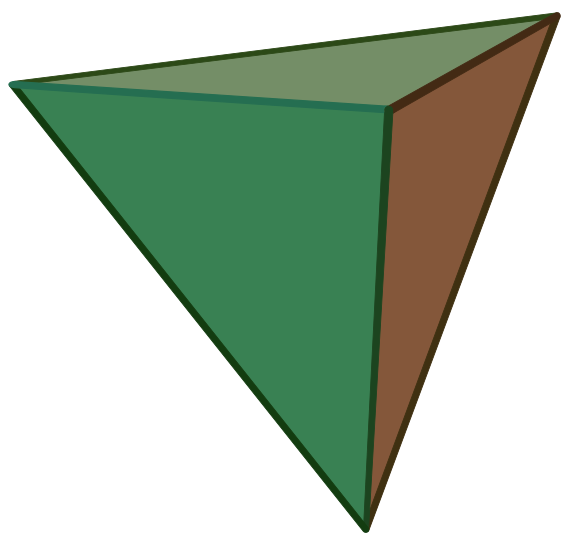
\includegraphics[width=0.25\marginparwidth]{SM/Tetrahedron.png}
\vspace*{-0.25cm}
\begin{center}\normalfont\small {Le Tétraèdre (le Feu).}\end{center}
\vspace*{-0.25cm}
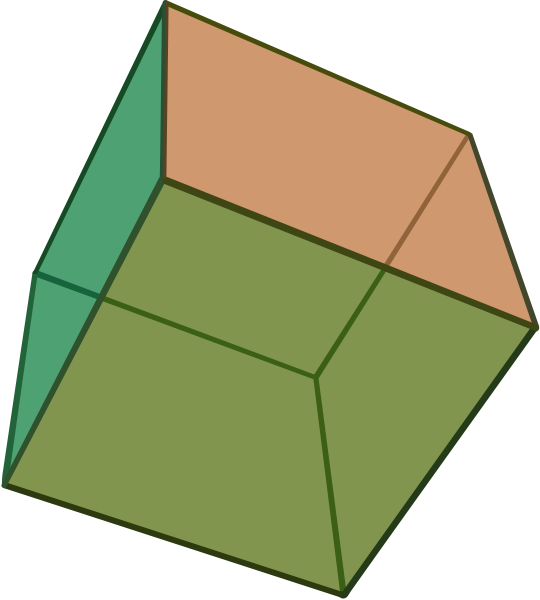
\includegraphics[width=0.25\marginparwidth]{SM/Hexahedron.png}
\vspace*{-0.25cm}
\begin{center}\normalfont\small {Le Cube (la Terre).}\end{center}
\vspace*{-0.25cm}
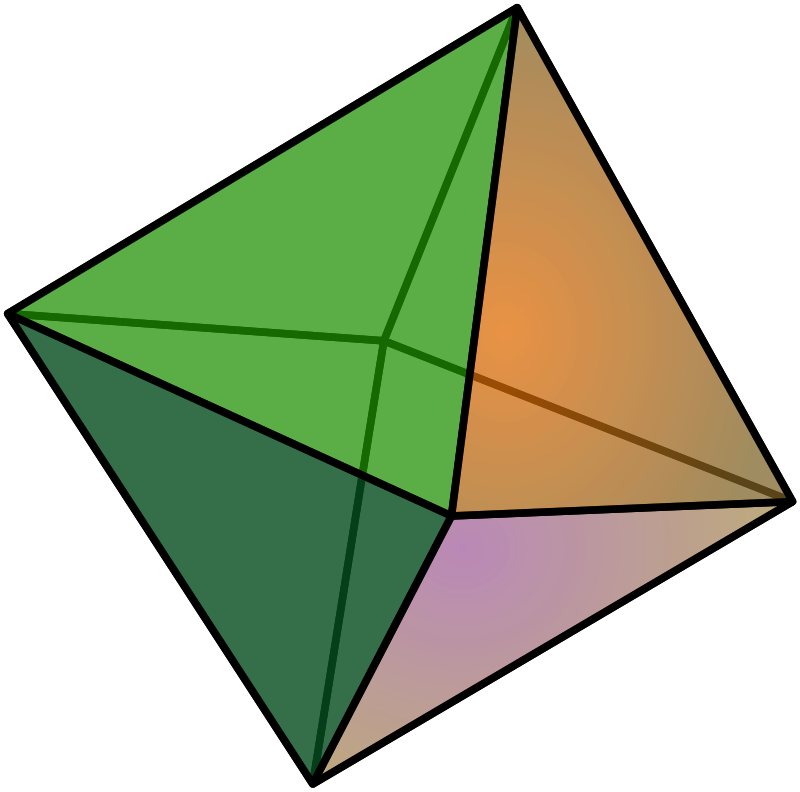
\includegraphics[width=0.25\marginparwidth]{SM/Octahedron.png}
\vspace*{-0.25cm}
\begin{center}\normalfont\small {L'Octaèdre (l'Air).}\end{center}
\vspace*{-0.25cm}
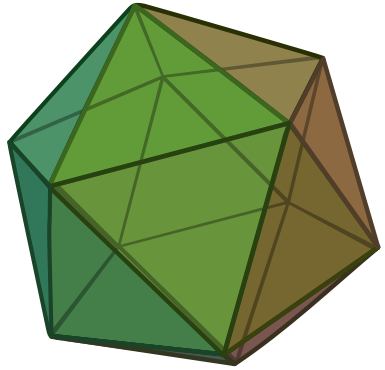
\includegraphics[width=0.25\marginparwidth]{SM/Icosahedron.png}
\vspace*{-0.25cm}
\begin{center}\normalfont\small {L'Icosaèdre (l'Eau).}\end{center}
\vspace*{-0.25cm}
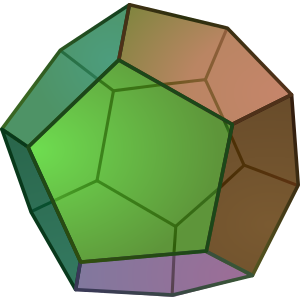
\includegraphics[width=0.25\marginparwidth]{SM/Dodecahedron.png}
\vspace*{-0.25cm}
\begin{center}\normalfont\small {Le Dodécaèdre (l'Univers).}\end{center}
\vspace*{-0.25cm}
\captionof{figure}{Les solides de Platon.}
\label{solides}
%\end{center}
}
De tout temps les hommes ont voulu comprendre et maitriser la nature. Cette quête a amené de nombreux penseurs, et notamment les philosophes Grecs, à proposer des explications sur le monde qui nous entoure, et certaines de leurs idées se révéleront florisantes et donneront naissance des siècles plus tard à la Physique en tant que science au sens moderne du mot. 

Anaxagore (~500-428 av. J.C.) pronait que toute chose est formée de particules élémentaires. Cette idée sera reprise par Empédocle (~495-~435 av J.C) qui proposa, l'eau, la terre, l'air et le feu comme étant ces particules. Platon (428/427 - 348/347 av. J.C.) associera ces quatres éléménts aux polygones réguliers convexes de l'espace à trois dimension (le tétraèdre pour le Feu, le cube pour la Terre, l'octaèdre pour l'Air, l'icosaèdre pour l'Eau, le dodécaère reprèsente l'éther, élément constituant l'Univers (fig.\ref{solides})). On doit à Leucippe (~460-~370 av J.C.) et son disciple Démocrite (~460-~370 av J.C.) le concept d'atomes qui composent la matière et sont indivisibles et séparés par du vide. La véracité de l'atomisme fera débat pendant des siècles et ne sera validé expérimentalement qu'au cours du XIX\ieme siècle.

 Parmis les travaux les plus importants qui prouverons l'existence des atomes, citons ceux de Lavoisier (1743-1794) qui décompose de nombreuses substances en "Éléments". De nombreux travaux sur les gaz, la cristallographie, la physique statistique et la thermodynamique : Bernoulli (1700-1782) : cinétique des gaz, Haüy (1743-1822) : La forme des cristaux reflète la symétrie des "briques élémentaires" le constituant , Dalton (1766-1844) : symbolisation des corps simples et des corps composés par des symboles auxquels il donne un poids de matière (fig.\ref{atom}), et liste des masses atomiques d'un certain nombre d'éléments rapportés à la masse de l'hydrogène, Gay-Lussac (1778-1850) : les rapports des volumes des réactifs et des produits de réaction sont des nombres entiers petits , Maxwell(1831-1879) : dispersion statistique des vitesses des molécules, Boltzmann (1844-1906) : répartition statistique des vitesses dans un gaz , Mendeleïev : Classification périodique des éléments et prédiction de nouveaux atomes (fig.\ref{periodique}). Ces travaux feront passer petit à petit cette théorie en réalité scientifique. 
 
\marginpar
{
	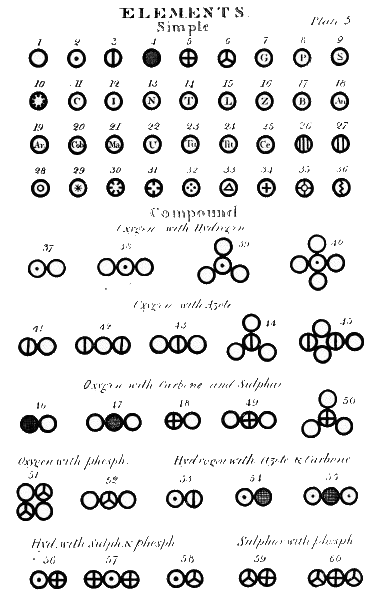
\includegraphics[width=\marginparwidth]{SM/Dalton.png}
    \captionof{figure}{Dessins de divers atomes et molécules tirés de l'ouvrage \textit{A New System of Chemical Philosophy}}
    	\label{atom}
}

\marginpar
{
	\vspace{2cm}
		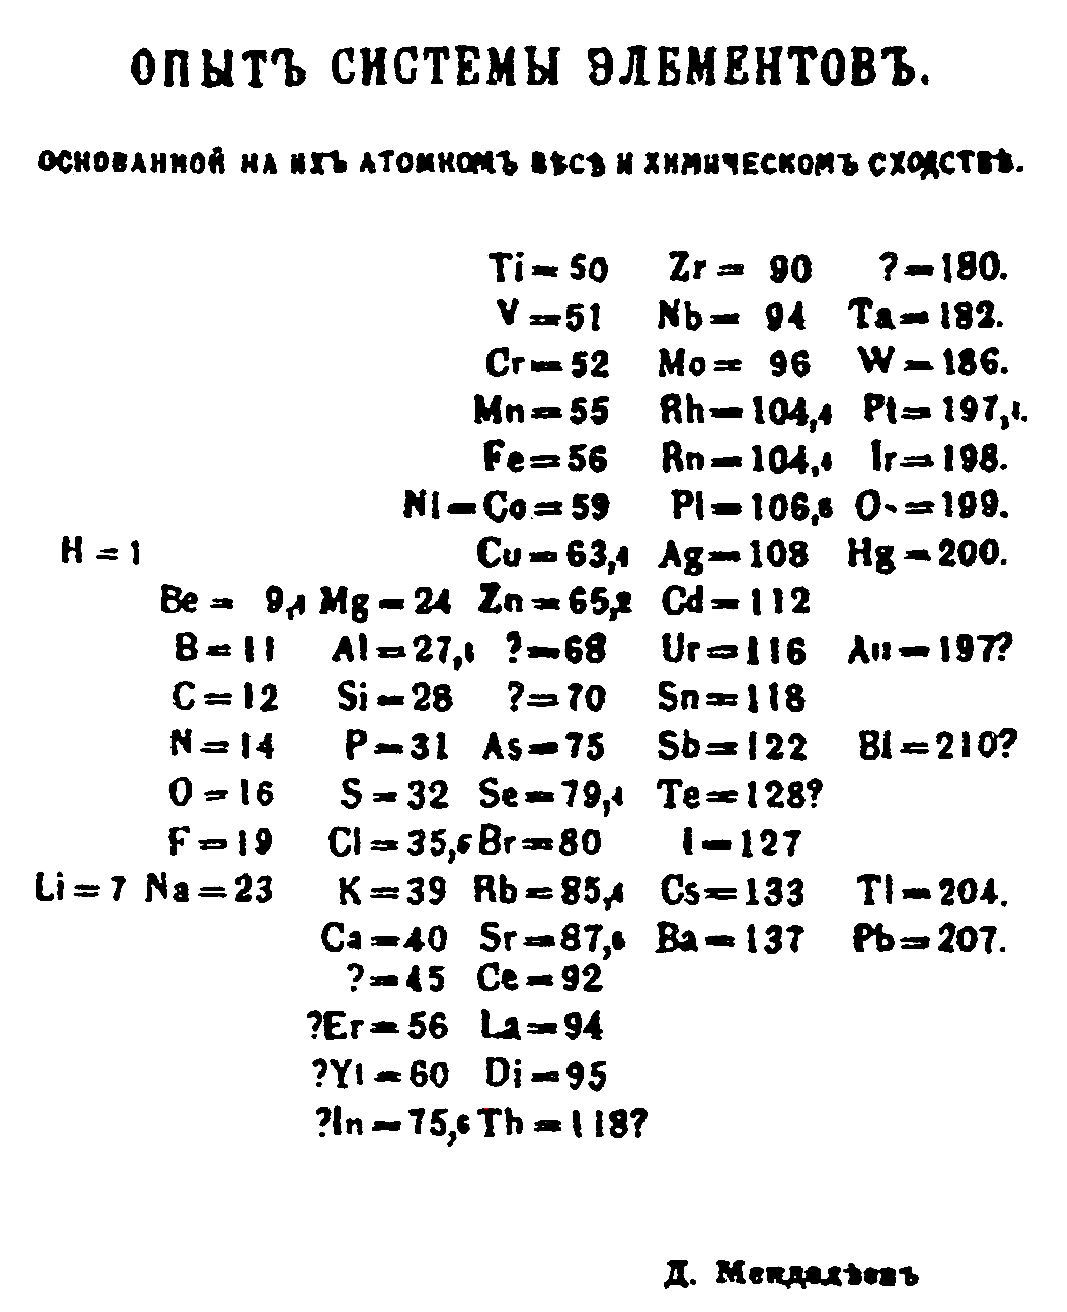
\includegraphics[width=\marginparwidth]{SM/periodique.png}
    \captionof{figure}{Tableau périodique de Mendeleïev}
    	\label{periodique}
}
D'autres domaine de la Physique connaitront des bouleversements importants au cours des siècles : 

Pour la Mécanique et la cosmologie : Copernic (1473-1543) et Galilée (1564-1642) : Modèle héliocentrique, Tycho Brahe (1546-1601) : remise en cause de  l'immuabilité du monde supra-lunaire énoncée par Aristote, Kepler (1571-1630) : Orbite elliptique des planètes, Newton (1643-1727) : théorie de la gravitation universelle, Lagrange (1736-1813) et Hamilton (1805-1865) : Principe de moindre action, Lagrangien, Hamiltonien.

Pour l'électromagnétisme : Coulomb(1736-1806) : loi de Coulomb, Volta(1745-1827): pile voltaïque, Ørsted (1777-1851), Ampère(1775-1836), Faraday(1792-1867), Henry (1797-1878) : les phénomènes d'induction, Maxwell : Équations de Maxwell.

Avec la découverte de l'électron par Thomson (1856-1940) en 1887 qui fût prédit en 1874 par Laming et Stoney. Thomson développe le premier modèle de l'atome, qui est décrit comme une boule de charge nulle possédant un noyau positif avec des électrons négatifs (modèle du "plum-pudding"). On découvre également durant cette période la radioactivité (Becquerel (1852-1908)). La physique semble à cette époque complète et cohérente. Lord Kelvin dira même dans son discours à la "Royal Institution of Great Britain" : \textit{"The beauty and clearness of the dynamical theory, which asserts heat and light to be modes of motion, is at present obscured by two clouds."}. Ces deux "nuages", l'incapacité à détecter l'éther luminifère  (expérience de Michelson-Morley) et la catastrophe ultraviolette du corps noir, donneront naissance respectivement à la relativité restreinte et à la mécanique quantique et feront entrer les physiciens dans la Physique Moderne.

Le début du siècle dernier sera une période florissante pour la physique des particules. Planck (1858-1947), afin de résoudre le problème du corps noir, proposera de quantifier les rayonnements : ceux-ci ne peuvent être qu'un multiple d'une constante qui porte son nom ($h$). Einstein ira plus loin et expliquera durant l'\textit{Annus mirabilis} (1905) l'effet photoélectrique en proposant le photon comme quanta de lumière qui agit comme une particule. Il possera également les bases de la relativité restreinte cette même année, réfutant le concept d'éther. De nombreux physiciens vont ensuite poser les bases de la mécanique quantique: Bohr (1885-1962), Compton (1892-1962), De Broglie (1892-1987), Schrödinger (1887-1961), Heisenberg (1901-1976), Dirac (1902-1984), Pauli (1900-1958). Avec les progrès tant théoriques qu'instrumentaux de Physiciens tels  Rutherford (1871-1937), Chadwick (1891-1974), Fermi (1901-1954), qui explorent le monde subatomique, on découvre les deux forces agissant à l'échelle du subatomique (les forces faible et forte) qui s'ajoutent aux deux force connues à l'époque (la force gravitationnelle et la force électromagnétique). Des physiciens tel Schwinger (1918-1994) veulent continuer la réunification des forces déjà avancée par les travaux de Maxwell ( force éléctrique et magnétique). Dans les années 1960, Weinberg (1933) et Salam (1926-1996) et Glashow (1932), réunissent dans une théorie dite électrofaible les forces électromagnétique et faible. Cette théorie prédit trois bosons ($W^{+}$, $W^{-}$ et $Z^{0}$). Leur théorie nécessite un boson supplémentaire, le boson de Higgs, postulé en 1964 par Brout, Englert, Higgs, Haggen Guralnik et Kibble afin de donner une masse aux particules. Cette théorie est la base du Modèle Standard de la physique des particules. La découverte des quarks amène à la création de la Chromodynamique Quantique (QCD) par Politzer (1949), Wilczek (1951), Gross (1941) afin de décrire l'interaction forte. Elle sera ensuite intégrée au Modèle Standard.

À partir de la seconde moitié du XX\ieme siècle, la Physique Subatomique a tâché de valider cette théorie et notamment par la découverte des bosons  $W^{+}$,$W^{-}$ et $Z^{0}$ en 1983, du quarks top $t$ en 1995, du neutrino tauique en 2000 et du boson de Higgs $h$ en 2012. De nombreux efforts sont également mené afin de continuer l'unification des forces entre elles. On sait cependant que le Modèle Standard, bien que jamais mis en défaut, ne peut tout expliquer. Certaines questions restent ouvertes et cette théorie présente même quelques défauts. La technicouleur, des modèles avec des dimensions supplémentaires ou la Supersymétrie sont des théories d'extension du Modèle Standard. Mais aucune n'a pu être encore validée expérimentalement.

\section{Le Modèle Standard de la physique des particules}
 
Au début du siècle dernier, tout tendait à faire croire que le monde était simplement composé d'atomes; eux mêmes constitués d'électron tournant autour d'un noyau composé de protons et neutrons. Tous les atomes connus avait été soigneusement classés dans le tableau périodique de Mendeleiev. Cependant, grâce à l'invention d'accélérateurs de particules linéaires, cyclotrons (fig. \ref{cyclo}) puis synchrotrons et l'observation des rayons cosmiques, les physiciens découvrirent bientôt qu'une pléthore de particules instables pouvaient être créées durant des désintégrations. Les Physiciens tentèrent bientôt de créer et classer ces particules en utilisant des énergies de faisceau de plus en plus grandes. Ce qui amena à la découverte d'une sous structure au sein même des nucléons\footnote{Protons et neutrons.} qui composent le noyau : les quarks (\ref{structure}).
\marginpar
{
	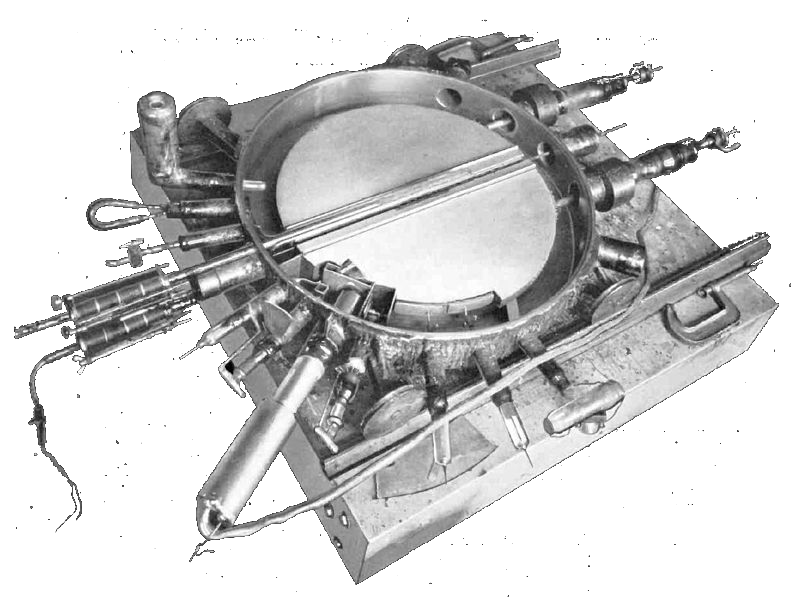
\includegraphics[width=\marginparwidth]{SM/cyclotron.png}
    \captionof{figure}{cyclotron de 27 pouces, accélérateur de $^{2}$H à 4 Mev (Université de Berkley, 1932).}
    	\label{cyclo}
}

\vspace*{-0.5cm}
\begin{figure}[h!]
\centering
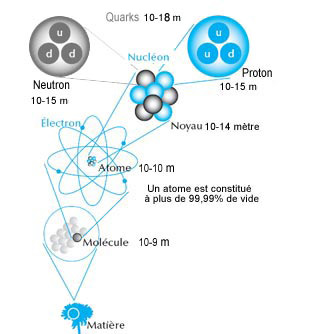
\includegraphics[width=0.50\textwidth]{SM/structure.jpg}
\captionof{figure}{Structure de la matière à différentes échelles.}
\label{structure}
\end{figure}

\vspace*{-0.5cm}
Parallèlement, de nouvelles interactions furent découvertes. Elles expliquaient les désintégrations radioactives ainsi que la cohésion des protons et des neutrons au sein du noyau atomique.

La physique des particules peut se résumer à la combinaison des deux démarches précédentes, à savoir, trouver les particules élémentaires ainsi que trouver les interactions fondamentales que ces particules peuvent subir. La manière dont ces particules interagissent aux moyens de ces interactions est donnée par la formulation mathématique d'une théorie, le Modèle Standard.

\subsection{Les particules élémentaires}
Les particules élémentaires du Modèle Standard, supposées indivisibles\footnote{à ce jour}, peuvent être classées en deux catégories selon leur spin (une propriété quantique intrinsèque à chaque particule) :
\begin{itemize}[label=$\bullet$]
\item les \textit{fermions}, ils constituent la matière et sont de spin demi-entier.
\item les \textit{bosons}, ils sont les messagers de l'interaction et sont de spin entier.
\end{itemize}
Chaque particule du Modèle Standard possède des nombres quantiques telles que sa masse, sa charge électrique, en fraction de l'opposé de la charge électrique de l'électron e par convention (e=$1.6\times10^{-19}$ C). Dans le cadre de la théorie, à chaque particule correspond une anti-particule\footnote{Une particule peut être sa propre anti-particule.} qui possède la même masse mais dont les nombres quantiques sont opposés.

\subsubsection{Les fermions}
Les fermions peuvent être classés en deux catégories selon qu'ils sont sensibles à l'interaction forte ou non. Dans le premier cas, ils font partis des \textit{quarks}, sinon ce sont des \textit{leptons}. Ces deux catégories sont elles-mêmes divisées en trois \textit{générations} (tab. \ref{fermions}).

Les leptons ont une charge électrique entière ($\pm$ 1) pour les électrons, muons et tau, et une charge nulle pour les neutrinos électroniques, neutrinos muoniques et neutrinos tauiques.

Les quarks ont une charge électrique fractionnaire. On associe à chaque quark un nombre quantique appelé "couleur" (Rouge, Vert et Bleu). Dû à la propriété de confinement de couleur, un quark ne peut être isolé et doit se combiner avec un ou deux autre quarks afin de former des \textit{mésons} (fig.\ref{mésons}) et des \textit{baryons} (fig.\ref{baryons}) respectivement. La somme des deux (trois) couleurs des quarks doit constituer un méson (baryon) "blanc" \footnote{Selon l'analogie avec la synthèse additive des couleurs.}. Les mésons et baryons sont regroupés sous le terme générique de \textit{hadrons}.

\marginpar
{
\centering

\includegraphics[width=\marginparwidth]{SM/quarks2.png}
\captionof{figure}{Un méson ($\pi^{+}$).}
\label{mésons}
}

\marginpar
{
	\centering
    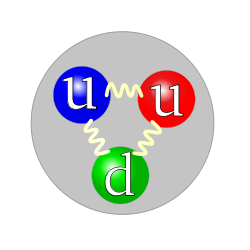
\includegraphics[width=\marginparwidth]{SM/quarks.png}
    \captionof{figure}{Un baryon ($p$).}
    	\label{baryons}
}
	
\marginpar
{
\centering
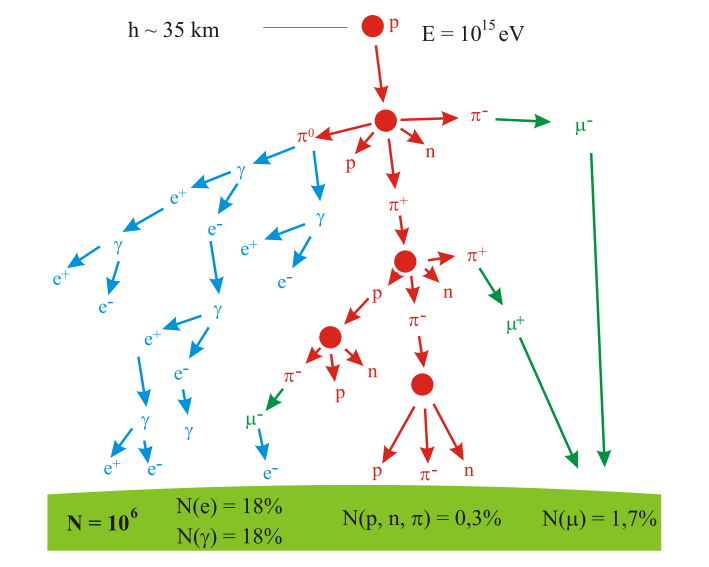
\includegraphics[width=0.95\marginparwidth]{SM/shower.png}
\captionof{figure}{Schéma d'une gerbe atmosphèrique.}
\label{gerbe}
}

La matière qui nous entoure n'est composée que de particules de la première génération. Tous les atomes sont composés d'électrons et de quarks $u$ et $d$ qui s'assemblent pour donner des protons $p$ et neutrons $n$. Les autres particules peuvent être créées si l'énergie disponible est suffisante (lors de gerbe atmosphérique où un proton vient interagir avec des particules de notre atmosphère par exemple \ref{gerbe} ou dans un collisionneur).
\definecolor{Orange}{HTML}{FFDD00}
\definecolor{Orange2}{HTML}{FFC000}
\definecolor{Green}{HTML}{8FB73E}
\definecolor{Green2}{HTML}{4EA700}
\definecolor{Red}{HTML}{EF4123}
\definecolor{Red2}{HTML}{EF2300}
\vspace*{1cm}
\begin{table}[H]
\centering
\begin{tabular}{|O|O|O|O|N}
\hline 
\rowcolor{Orange2}Quarks & 1\iere génération & 2\ieme génération & 3\ieme génération \\
\hline 
\cellcolor{Orange2} Nom &\cellcolor{Orange} Up & \cellcolor{Orange} Charm &  \cellcolor{Orange} Top \\
\cellcolor{Orange2} Notation &\cellcolor{Orange} $u$,$\bar{u}$ & \cellcolor{Orange} $c$,$\bar{c}$ &  \cellcolor{Orange} $t$,$\bar{t}$ \\
\cellcolor{Orange2} Charge &\cellcolor{Orange} $\pm \frac{2}{3}$ & \cellcolor{Orange} $\pm \frac{2}{3}$ &  \cellcolor{Orange} $\pm \frac{2}{3}$ \\
\cellcolor{Orange2} Masse &\cellcolor{Orange} $0.005$ GeV/c$^2$ & \cellcolor{Orange} $1.35$ GeV/c$^2$ &  \cellcolor{Orange} $172.6$ GeV/c$^2$ \\
\hline 
\cellcolor{Orange2} Nom &\cellcolor{Orange} Down & \cellcolor{Orange} Strange &  \cellcolor{Orange} Bottom \\
\cellcolor{Orange2} Notation &\cellcolor{Orange} $d$,$\bar{d}$ & \cellcolor{Orange} $s$,$\bar{s}$ &  \cellcolor{Orange} $b$,$\bar{b}$ \\
\cellcolor{Orange2} Charge &\cellcolor{Orange} $\mp \frac{1}{3}$ & \cellcolor{Orange} $\mp \frac{1}{3}$ &  \cellcolor{Orange} $\mp \frac{1}{3}$ \\
\cellcolor{Orange2} Masse &\cellcolor{Orange} $0.01$ GeV/c$^2$ & \cellcolor{Orange} $0.1$ GeV/c$^2$ &  \cellcolor{Orange} $1.3$ GeV/c$^2$ \\
\hline 
\rowcolor{Green2} Leptons & 1\iere génération & 2\ieme génération & 3\ieme génération \\
\hline
\cellcolor{Green2} Nom & \cellcolor{Green} Électron & \cellcolor{Green} Muon & \cellcolor{Green} Tau \\
\cellcolor{Green2} Notation & \cellcolor{Green} $e^{\pm}$ & \cellcolor{Green} $\mu^{\pm}$ & \cellcolor{Green} $\tau^{\pm}$ \\
\cellcolor{Green2} Charge & \cellcolor{Green} $\pm 1$ & \cellcolor{Green} $\pm 1$ & \cellcolor{Green} $\pm 1$ \\
\cellcolor{Green2} Masse & \cellcolor{Green} $0.511$ MeV/c$^2$ & \cellcolor{Green} $105.7$ MeV/c$^2$ & \cellcolor{Green} $1777$ MeV/c$^2$ \\
\hline 
\cellcolor{Green2} Nom & \cellcolor{Green} Neutrino électronique & \cellcolor{Green} Neutrino muonique & \cellcolor{Green} Neutrino tauique \\
\cellcolor{Green2} Notation & \cellcolor{Green} $\nu_{e}$ & \cellcolor{Green} $\nu_{\mu}$ & \cellcolor{Green} $\nu_{\tau}$ \\
\cellcolor{Green2} Charge & \cellcolor{Green} $0$ & \cellcolor{Green} $0$ & \cellcolor{Green} $0$ \\
\cellcolor{Green2} Masse & \cellcolor{Green} $<0.017$ MeV/c$^2$ & \cellcolor{Green} $<0.27$ MeV/c$^2$ MeV/c$^2$ & \cellcolor{Green} $<35$ MeV/c$^2$ \\

\hline
\end{tabular} 
\captionof{table}{Fermions: Quarks et Leptons.}
\label{fermions}
\end{table}	

\subsubsection{Les bosons}
La description perturbative du Modèle Standard utilise l'échange de bosons virtuelles, afin de décrire l'interaction entre deux particules. Les bosons sont les médiateurs des interactions. Les particules de matière (fermions) interagissent donc entre elles par l'échange de particules de spin 1 correspondant à la force responsable de leur interaction.
\smallskip
Chacune des quatre interactions possède donc un ou plusieurs bosons appelés bosons de jauge (bosons vecteurs) (Tab.\ref{bosons}) :

\marginpar
{
\begin{center}
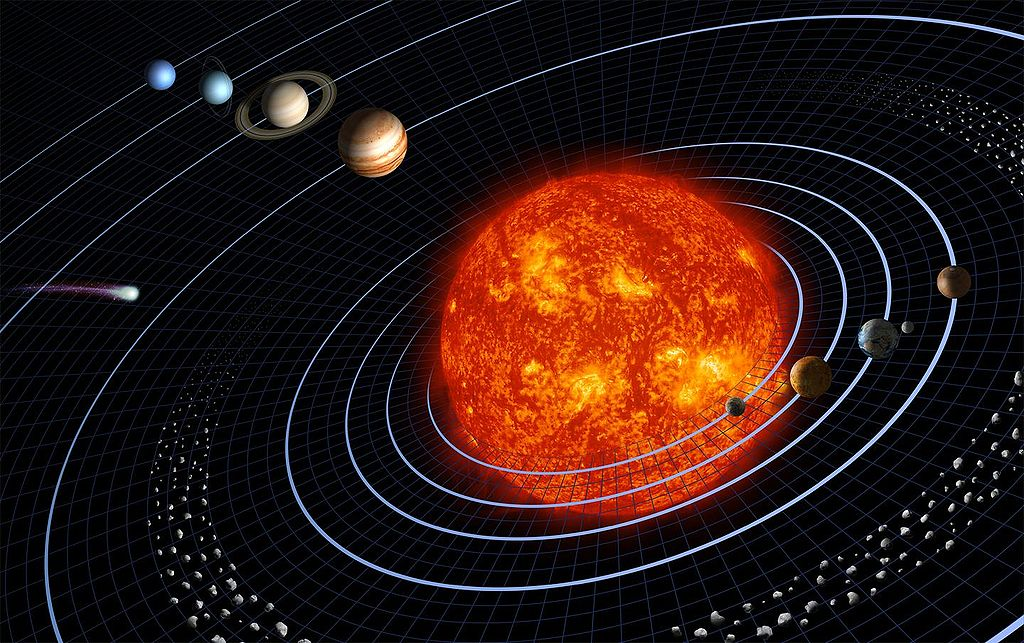
\includegraphics[width=\marginparwidth]{SM/solaire.jpg}
\begin{center}\normalfont\small {(a) Gravité : Système solaire.}\end{center}
\end{center}
}

\marginpar
{
\centering
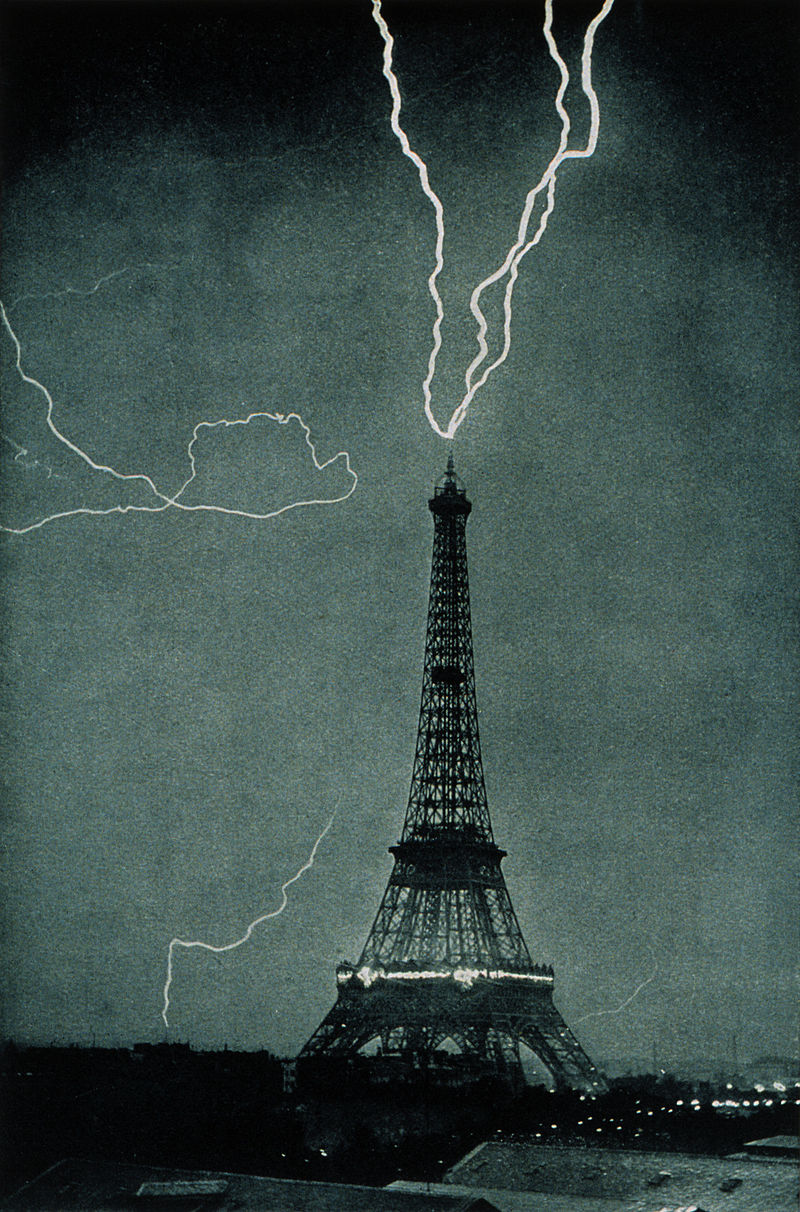
\includegraphics[width=\marginparwidth]{SM/foudre.jpg}
\begin{center}\normalfont\small {(b) Électromagnétisme : la foudre.}\end{center}
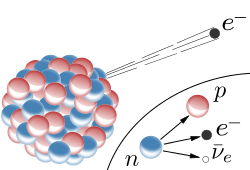
\includegraphics[width=\marginparwidth]{SM/beta.png}
\begin{center}\normalfont\small {(c) Interaction faible : désintégration $\beta$.}\end{center}
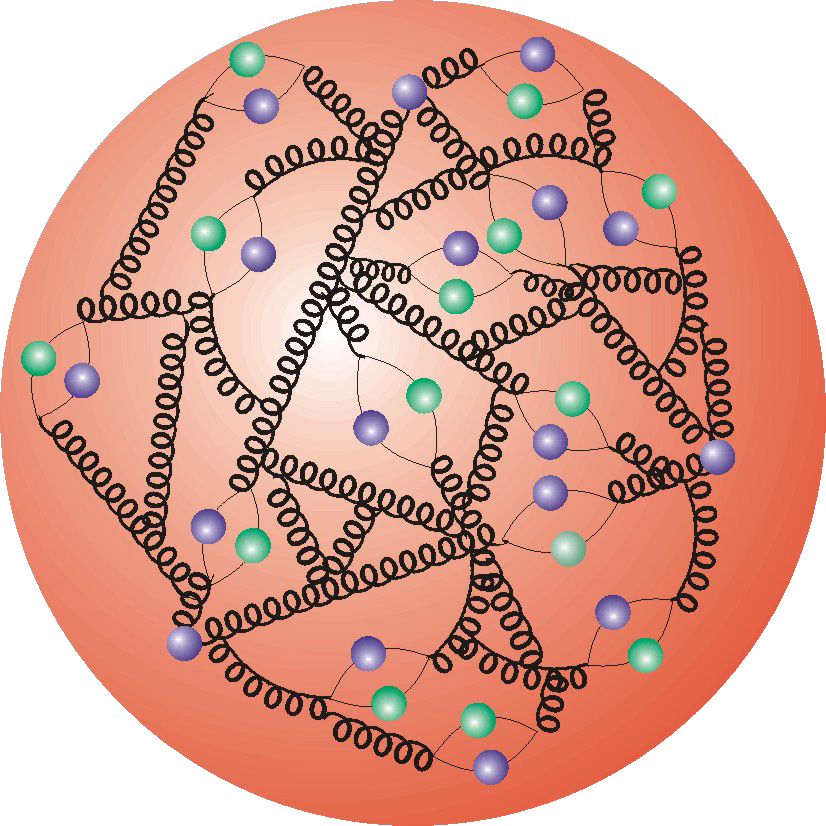
\includegraphics[width=0.8\marginparwidth]{SM/quarks3.png}
\begin{center}\normalfont\small {(d) Interaction forte : confinement.}\end{center}
\captionof{figure}{Exemple d'effets des 4 interactions.}
}

\begin{itemize}[label=$\bullet$]
\item \textbf{L'interaction gravitationnelle} est la première à avoir été découverte et expliquée (Galilée, Newton). Elle est négligeable à l'échelle atomique. Elle est gouvernée par la masse des corps mise en jeu et elle domine à grande échelle ( Univers, Galaxies, Planètes), son rayon d'action est infini. Sa description quantique repose sur un boson de spin 2 qui est encore activement recherché. Un pas décisif à été fait grâce à la détection par les expériences Virgo et Ligo des ondes Gravitationnelle. Cette interaction est la seule à ne pas être intégrée au Modèle Standard. Elle est actuellement décrite par la Relativité Générale qui est une approche non quantique.

\item \textbf{L'interaction électromagnétique} gouverne les interactions entre les particules chargées. C'est l'une des interactions qui nous est la plus familière car elle est prépondérante dans notre vie quotidienne ( lumière, chimie, frottements ...). Tout comme la gravité, son rayon d'action est infini. Son boson médiateur est le photon $\gamma$.

\item \textbf{L'interaction faible} à été découverte et comprise à travers la désintégration de particules avec changements de saveurs. Elle fait passer d'un fermion à un autre (par exemple lors de la désintégration $\beta$, elle transforme un neutron en un proton en changeant un quark $d$ en un quark $u$ avec la création d'un neutrino et d'un électron). Les bosons médiateurs de l'interaction sont les bosons $W^{+}$ $W^{-}$ $Z^{0}$. Sa portée est de l'ordre de 10$^{-18}$ m due à la masse des bosons médiateur.

\item \textbf{L'interaction forte} permet l'échange de couleur entre les quarks et la création et l'annihilation de particules. Elle est responsable de la cohésion du noyau, et elle lie les nucléons entre eux à l'intérieur du noyau atomique. Ses bosons médiateur sont les gluons et sont au nombre de huit. Bien que les gluons soient supposés de masse nulle, la portée de l'interaction est de l'ordre de 10$^{-15}$ m. Cette portée est la conséquence du principe de confinement de couleur qui affecte les quarks. En effet, cette interaction a la propriété de voir son intensité augmenter avec la distance, ce qui à tendance à regrouper les quarks entre eux. Cette propriété est également responsable du processus d'hadronisation des quarks et de la création de jets.
\end{itemize}

\vspace{1cm}
\begin{table}[h!]
\centering
\begin{tabular}{|O|O|O|O|N}
\hline 
\rowcolor{Red2}Interaction&Rayon d'action&Bosons de jauge&Masses\\
\hline 
\cellcolor{Red}\shortstack{ Forte }&
\cellcolor{Red}\shortstack{ $2.5\times10^{-15}$ m}& 
\cellcolor{Red}\shortstack{  Gluons (8)}&
\cellcolor{Red}\shortstack{ 0}\\
\hline 
\cellcolor{Red}\shortstack{ Electromagnétique }&
\cellcolor{Red}\shortstack{ $\infty$}& 
\cellcolor{Red}\shortstack{Photon $\gamma$}&
\cellcolor{Red}\shortstack{0}\\
\hline 
\cellcolor{Red}\shortstack{Faible}&
\cellcolor{Red}\shortstack{$10^{-18}$ m }& 
\cellcolor{Red}\shortstack{$W^{\pm}$,$Z^{0}$}&
\cellcolor{Red}\shortstack{$80.399$,$91.188$ Gev/c$^{2}$}\\
\hline 
\cellcolor{Red}\shortstack{Gravitationnelle}&
\cellcolor{Red}\shortstack{$\infty$}& 
\cellcolor{Red}\shortstack{(Graviton)}&
\cellcolor{Red}\shortstack{(inconnue)}\\
\hline 
\end{tabular} 
\captionof{table}{Bosons : Interactions.}
\label{bosons}
\end{table}

\subsubsection{Le boson de Higgs}
Le boson de Higgs ($H^{0}$) est nécessaire afin de donner la masse des bosons $W^{\pm}$, $Z^{0}$ et des fermions. Bien que postulé en 1964, il n'a été découvert qu'en 2012 par les expériences CMS et ATLAS en 2012. Contrairement au bosons vecteur, le boson de Higgs est de spin 0.
\newpage
Toutes ces particules peuvent être résumer dans le tableau suivant : 

\begin{minipagewithmarginpars}[h]{\textwidth}
\vspace{-0.5cm}
\centering
\hspace*{-1.5cm}
\includestandalone{./SM/bestiaire}
\captionof{figure}{Classification des quarks, leptons et bosons.}
\label{bestiaire}
\marginpar
{
\vspace*{1.5cm}
%\begin{center}
\centering

\includegraphics[width=\marginparwidth]{SM/feyn0.png}
\begin{center}\normalfont\small {(a) Développement à l'arbre.}\end{center}
%\end{center}
}
\end{minipagewithmarginpars}
\subsection{Le formalisme du Modèle Standard}
\marginpar
{
\centering

\includegraphics[width=\marginparwidth]{SM/feyn1.png}

\includegraphics[width=\marginparwidth]{SM/feyn2.png}

\includegraphics[width=\marginparwidth]{SM/feyn3.png}
\begin{center}\normalfont\small {(b) Développement à l'ordre 1.}\end{center}
\captionof{figure}{Exemple de diagrammes de Feynman pour le développement en série de la diffusion électron-électron.}
\label{feyn}
}
Le Modèle Standard est une théorie non-abélienne où les interactions sont régis par des symétries locales de jauge. Elle repose sur la théorie quantique des champs qui permet de décrire les particules et leurs interactions. Cette théorie est à la fois quantique et relativiste. Elle permet donc de caractériser les interactions par des probabilités de transition d'un état initial à un état final, ainsi que de rendre compte du temps de propagation des interactions, la description des particules à hautes énergie et les créations annihilation de particules.

Dans cette théorie, à chaque type de particule est associé un champ $\psi(\vec{x},t)$ et les interactions sont liées à des propagateurs. La création (l'annihilation) de particules est associé à des opérateurs qui excitent(désexciter) le champ de particules à une position $\vec{x}$ et à un temps $t$. L'un des postulat de la théorie quantique des champs est que l'ensemble des informations de la théorie est contenu dans un Lagrangien $\mathcal{L}$ qui s'exprime en fonction des champs et de leurs dérivées. Il est possible, à partir de ce Lagrangien d'obtenir les équations de mouvements en minimisant sont action $S=\int\mathcal{L}\Diff4{x}$.
Le Modèle Standard et une théorie perturbative, c'est à dire que les observables sont calculées par une méthode qui s'appuie sur un développement en série dont la précision augmente avec l'ordre. Au premier ordre, l'observable est dite être calculé à l'arbre ou LO (Leading Order). Ce développement en série n'est valable que si les constantes de couplage des interactions reste faible devant l'unité. Ce développement en série peut être schématisé grâce aux diagrammes de Feynmann (fig. \ref{feyn}), qui sont des diagramme représentant des règles de calculs. Chaque types de particules et d'interactions posséde son symbole et à chaque particules doit être connécté par un vertex (représentant une interactions).

Le principe selon lequel les interactions sont gouvernés par des symétries est également un postulat des important du Modèle Standard. De par le théorème de Noether, les symétries continues sont liées à des quantités physique qui se conserve. Le Modèle Standard est basé sur le produit direct du groupe de la chromodynamique quantique, décrivant l'interaction forte, qui impose une conservation de la charge de couleur, $SU(3)_{C}$ et du groupe de la théorie électrofaible, $SU(2)_{L} \otimes U(1)_{Y}$, imposant une symétrie locale de l'isospin $I$ associé au groupe $SU(2)_{L}$ et une symètrie locale de l'hypercharge $Y$ du groupe $U(1)_{Y}$.

\subsection{Lagrangien du modèle standard}
Le modèle standard est une théorie de Jauge qui se base sur le groupe $SU(3)_{C} \otimes SU(2)_{L} \otimes U(1)_{Y}$ dont le lagrangien peut s'écrire sous la forme :

\begin{equation}
\mathcal{L_{MS}}=\mathcal{L}_{\mathrm{Yang-Mills}}+\mathcal{L}_{\mathrm{Dirac}}+\mathcal{L}_{\mathrm{Yukawa}}+\mathcal{L}_{\mathrm{Higgs}}
\end{equation}

\subsubsection{Le terme de Yang-Mills (secteur de jauge)}
Le secteur de jauge est la partie cinématique des champs de jauge :
\begin{equation}
\mathcal{L}_{\mathrm{Yang-Mills}}=-\frac{1}{4}B_{\mu\nu}B^{\mu\nu}-\frac{1}{4}W_{\mu\nu}^{a}W_{a}^{\mu\nu}-\frac{1}{4}G_{\mu\nu}^{A}G_{A}^{\mu\nu}
\end{equation}
où 
\begin{equation}
B_{\mu\nu}=\partial_{\mu}B_{\nu}-\partial_{\nu}B_{\mu}
\end{equation}
avec $B_{\mu}$ le champ isoscalaire associé au groupe d'hypercharge $U(1)_{Y}$,
\begin{equation}
W_{\mu\nu}^{a}=\partial_{\mu}W_{\nu}^{a}-\partial_{\nu}W_{\mu}^{a}+g\epsilon_{abc}W_{\mu}^{b}W_{\nu}^{c}
\end{equation}
où $W_{\mu}^{a} (a=1,2,3)$ est le triplet d'isospin I=1 du groupe de l'isospin faible $SU(2)_{L}$, g la constante de couplage de l'isospin faible et $\epsilon_{abc}$ les constantes de structures antisymétriques correspondantes.  
\begin{equation}
G_{\mu\nu}^{A}=\partial_{\mu}G_{\nu}^{A}-\partial_{\nu}G_{\mu}^{A}+g'\epsilon_{ABC}G_{\mu}^{B}G_{\nu}^{C}
\end{equation}
les champs des gluons $G_{\mu}^{A} (A=1,2,..,8)$, bosons vecteurs de $SU(3)_{c}$, $g'$ la constante de couplage de couleur et $f_{ABC}$ les constantes de structures de $SU(3)_{C}$.
La nature non-Abélienne de $SU(2)_{L}$ et $SU(3)_{c}$ amène à des termes supplémentaires dans l'écriture des champs du triplet d'isospin et des champs de gluons. Ce sont ces termes qui sont reponsables de l'interaction des bosons $W$ et des gluons $g$.

\subsubsection{Le secteur de Dirac}
Le secteur de Dirac décrit les interactions des fermions avec les bosons de jauge. Dans le secteur électrofaible, les fermions se regroupent de manière asymétrique dans des doublets d'isospin faible de chiralité gauche et dans des singulets de chiralité droite (tab. \ref{doublets}). Il y a violation maximale de la parité de $SU(2)_{L}\otimes U(1)_{Y}$

\begin{table}[H]
\centering
\begin{tabular}{|L|L|} 
\hline
\multicolumn{2}{|Cc|}{Quarks} \\
\hline
Gauches $Q_{\alpha L}^{i}$ & $\begin{pmatrix} 
u^{i}\\
d^{i}
\end{pmatrix}_{L},\ \begin{pmatrix} 
c^{i}\\
s^{i}
\end{pmatrix}_{L},\ \begin{pmatrix} 
t^{i}\\
b^{i}
\end{pmatrix}_{L}$ \\
\hline
Droits $Q_{\beta R}^{i}$&$ u_{iR},\ d_{iR},\ c_{iR},\ s_{iR},\ t_{iR},\ b_{iR}$\\
\hline
\multicolumn{2}{|Cc|}{Leptons} \\
\hline
Gauche $L_{\alpha L}$& $\begin{pmatrix} 
\nu_{e}\\
e
\end{pmatrix}_{L},\ \begin{pmatrix} 
\nu_{\mu}\\
\mu
\end{pmatrix}_{L},\ \begin{pmatrix} 
\nu_{\tau}\\
\tau
\end{pmatrix}_{L} $\\
\hline
Droits $L_{\gamma R}$& $e_{R},\ \mu_{R},\ \tau_{R},\ \left(\nu_{e R},\ \nu_{\mu R},\ \nu_{\tau R}\right)$ \\
\hline
\end{tabular}
\captionof{table}{Doublets et singulets pour $SU(2)_{L}$ ;$i$=1,2,3 couleurs, $\alpha$=1,2,3 familles, $\beta$={u,d,s,c,t,b}, $\gamma$={$e$,$\mu$,$\tau$,$\left(\nu_{e},\nu_{\mu},\nu_{\tau}\right)$}}.
\label{doublets}
\end{table}	

En suivant ces notations le secteur de Dirac du Lagrangien du Modèle Standard s'écrit:
\marginpar
{
\begin{equation*}
\sigma_{1}=\begin{pmatrix} 
0&1\\
1&0\\
\end{pmatrix}
\end{equation*}
\vspace{0.2cm}
\begin{equation*}
\sigma_{2}=\begin{pmatrix} 
0&-i\\
i&0\\
\end{pmatrix}
\end{equation*}
\vspace{0.2cm}
\begin{equation*}
\sigma_{3}=\begin{pmatrix} 
1&0\\
0&-1\\
\end{pmatrix}
\end{equation*}
\captionof{figure}{Les matrices canoniques de Pauli.}
\label{Pauli}
}
\marginpar
{
\begin{equation*}
\lambda_{1}=\begin{pmatrix} 
0&1&0\\
1&0&0\\
0&0&0
\end{pmatrix}
\end{equation*}
\vspace{0.2cm}
\begin{equation*}
\lambda_{2}=\begin{pmatrix} 
0&-i&0\\
i&0&0\\
0&0&0
\end{pmatrix}
\end{equation*}
\vspace{0.2cm}
\begin{equation*}
\lambda_{3}=\begin{pmatrix} 
1&0&0\\
0&-1&0\\
0&0&0
\end{pmatrix}
\end{equation*}
\vspace{0.2cm}
\begin{equation*}
\lambda_{4}=\begin{pmatrix} 
0&0&1\\
0&0&0\\
1&0&0
\end{pmatrix}
\end{equation*}
\vspace{0.2cm}
\begin{equation*}
\lambda_{5}=\begin{pmatrix} 
0&0&-i\\
0&0&0\\
i&0&0
\end{pmatrix}
\end{equation*}
\vspace{0.2cm}
\begin{equation*}
\lambda_{6}=\begin{pmatrix} 
0&0&0\\
0&0&1\\
0&1&0
\end{pmatrix}
\end{equation*}
\vspace{0.2cm}
\begin{equation*}
\lambda_{7}=\begin{pmatrix} 
0&0&0\\
0&0&-i\\
0&i&0
\end{pmatrix}
\end{equation*}
\vspace{0.2cm}
\begin{equation*}
\lambda_{8}=\frac{1}{\sqrt{3}}\begin{pmatrix} 
1&0&0\\
0&1&0\\
0&0&-2
\end{pmatrix}
\end{equation*}
\captionof{figure}{Les matrices canoniques de Gell-Mann.}
\label{Gell-Mann}
}

\begin{equation}
\begin{split}
\mathcal{L}_{\mathrm{Dirac}}=&i\sum_{\alpha=1}^{3}\bar{L}_{\alpha L}\gamma_{\mu}D_{L_{L}}^{\mu}L_{\alpha L}+\sum_{\gamma=1}^{3(6)}\bar{L}_{\gamma R}\gamma_{\mu}D_{L_{R}}^{\mu}L_{\gamma R}\\
&+\sum_{\alpha=1}^{3}\sum_{i=1}^{3}\bar{Q}_{\alpha L}^{i}\gamma_{\mu}D_{Q_{L}}^{\mu}Q_{\alpha L}^{i}+\sum_{\beta=1}^{6}\sum_{i=1}^{3}\bar{Q}_{\beta R}^{i}\gamma_{\mu}D_{Q_{R}}^{\mu}Q_{\beta R}^{i}
\end{split}
\end{equation}
Avec les dérivées covariantes de la forme : 
\begin{equation}
D_{\mu L_{L}}=\partial_{\mu} -ig\frac{\sigma^a}{2}W_{\mu}^{a}-ig'\frac{Y^{W}_{L}}{2}B_{\mu}
\end{equation}
\begin{equation}
D_{\mu L_{R}}=\partial_{\mu} -ig'\frac{Y^{W}_{R}}{2}B_{\mu}
\end{equation}
\begin{equation}
D_{\mu Q_{L}}=\partial_{\mu} -ig\frac{\sigma^a}{2}W_{\mu}^{a}-ig'\frac{Y^{W}_{L}}{2}B_{\mu}-ig''\frac{\lambda^{A}}{2}Q_{\mu}^{A}
\end{equation}
\begin{equation}
D_{\mu Q_{R}}=\partial_{\mu}ig'\frac{Y^{W}_{R}}{2}B_{\mu}-ig''\frac{\lambda^{A}}{2}Q_{\mu}^{A}
\end{equation}
où $\sigma^{a}$ sont les générateur de $SU(2)_{L}$ (matrices de Pauli (Fig. \ref{Pauli})), $\lambda^{A}$ les générateurs de $SU(3)_{c}$ (matrices de Gell-Mann (Fig. \ref{Gell-Mann})) et $Y^{W}$, l'hypercharge faible, le générateur de $U(1)_{Y}$. 
Afin d'obtenir les charges électriques pour chaque fermions, on pose:
\begin{multline}
\begin{split}
&Y^W(L_{\alpha L})=-1,\ &Y^W(e_{R},\mu_{R},\tau_{R})=-2,\ &\left(Y^W(\nu_{e R},\nu_{\mu R},\nu_{\tau R})=0\right)\\
&Y^W(Q_{\alpha L})=\frac{1}{3},\ &Y^W(u_{R},c_{R},t_{R})=\frac{4}{3},\ &Y^W(d_{R},s_{R},b_{R})=-\frac{2}{3}
\end{split}
\end{multline}  

\subsubsection{Le secteur de Higgs} 
La symétrie électrofaible est incompatible avec la description de fermion massif. En effet, dans le Lagrangien les termes de masses des fermions sont de la forme 
\begin{equation}
\mathcal{L_{M}}=-m\bar{\phi}\phi=-m \left(\phi_{L}^{\dagger}\phi_{R}+\phi_{R}^{\dagger}\phi_{L}\right)
\end{equation}
Cependant, ces termes brisent la symétrie $SU(2)$ et n'est donc pas inclus dans le Lagrangien. De plus, l'expérience montre que les bosons de jauge $W$ doivent posséder une masse. Or l'introduction des termes de masses pour ces boson est également impossibles pour les mêmes raisons.

Afin de résoudre ces problèmes, on introduit un champ scalaire complexe $\phi$, doublet de $SU(2)_{L}$ de quatre champs réels $\phi_{i}$ et d'hypercharge $Y=1$ :
\begin{equation}
\phi=\begin{pmatrix} 
\phi^{+}\\
\phi^{0}
\end{pmatrix}=\frac{1}{\sqrt{2}}\begin{pmatrix} 
\phi_{1}+\phi_{2}\\
\phi_{3}+\phi_{4}
\end{pmatrix}
\end{equation}
On utilise l'expression du Lagrangien la plus générale pour un champ scalaire complexe de $SU(2)$:
\begin{equation}
\mathcal{L}_{\mathrm{Higgs}}=\left(D_{\mu}\phi\right)^{\dagger}\left(D^{\mu}\phi\right)-V(\phi),
\end{equation}
avec 
\begin{equation}
D_{\mu}=\partial_{\mu} -ig\frac{\sigma^a}{2}W_{\mu}^{a}-ig'\frac{Y}{2}B_{\mu}.
\end{equation}
Afin que le lagrangien $\mathcal{L}_{\mathrm{Higgs}}$ soit invariant globalement, le potentiel scalaire $V(\phi)$ ne doit pas comporter de puissance impaires de $\phi$. De plus, afin que la théorie reste renormalisable, les puissances au delà de $\phi^4$ sont à proscrire.

Le potentiel $V(\phi)$ est donc de la forme :
\begin{equation}
V(\phi)=\mu^{2}\phi^{\dagger}\phi+\lambda\left(\phi^{\dagger}\phi\right)^2,
\end{equation}
et a un profil différent selon les signes de $\mu^{2}$ et de $\lambda$ (Fig. \ref{profile}).
\marginpar{ 
\resizebox {\marginparwidth} {!} 
{
\begin{tikzpicture}
\begin{axis}[view={15}{15},yticklabels={,,},xticklabels={,,},zticklabels={,,},mesh/interior colormap name=hot,colormap/blackwhite]
\addplot3[surf,shader=faceted,samples=50,fill opacity=0.5,opacity=0.4,domain=0:1.05,y domain=0:2*pi,z buffer=sort]({x * cos(deg(y))}, {x * sin(deg(y))}, {-x*x-x*x*x*x});
\end{axis}
\end{tikzpicture}
}
\begin{center}\normalfont\small {(a) $\mu^{2}<0$ , $\lambda<0$.}\end{center}
\resizebox {\marginparwidth} {!} 
{
\begin{tikzpicture}
\begin{axis}[view={15}{15},yticklabels={,,},xticklabels={,,},zticklabels={,,},mesh/interior colormap name=hot,colormap/blackwhite]
\addplot3[surf,shader=faceted,samples=50,fill opacity=0.5,opacity=0.4,domain=0:1.05,y domain=0:2*pi,z buffer=sort]({x * cos(deg(y))}, {x * sin(deg(y))}, {+x*x+x*x*x*x});
\end{axis}
\end{tikzpicture}
}
\begin{center}\normalfont\small {(b) $\mu^{2}>0$ , $\lambda>0$.}\end{center}
\resizebox {\marginparwidth} {!} 
{
\begin{tikzpicture}
\begin{axis}[view={15}{15},yticklabels={,,},xticklabels={,,},zticklabels={,,},mesh/interior colormap name=hot,colormap/blackwhite]
\addplot3[surf,shader=faceted,samples=50,fill opacity=0.5,opacity=0.4,domain=0:1.05,y domain=0:2*pi,z buffer=sort]({x * cos(deg(y))}, {x * sin(deg(y))}, {+x*x-x*x*x*x});
\end{axis}
\end{tikzpicture}
}
\begin{center}\normalfont\small {(c) $\mu^{2}>0$ , $\lambda<0$.}\end{center}
\resizebox {\marginparwidth} {!} 
{
\begin{tikzpicture}
\begin{axis}[view={15}{15},yticklabels={,,},xticklabels={,,},zticklabels={,,},mesh/interior colormap name=hot,colormap/blackwhite]
\addplot3[surf,shader=faceted,samples=50,fill opacity=0.5,opacity=0.4,domain=0:1.05,y domain=0:2*pi,z buffer=sort]({x *cos(deg(y))},{x*sin(deg(y))},{-x*x+x*x*x*x});
\end{axis}
\end{tikzpicture}
}
\begin{center}\normalfont\small {(d) $\mu^{2}<0$ , $\lambda>0$.}\end{center}
\captionof{figure}{Les différents profils de $V(\phi)$ selon les signes de $\mu^{2}$ et $\lambda$.}
\label{profile}
}
Les cas où $\mu^{2}>0$ ne possède qu'un minimum en $0$, ce qui est inutile. Le cas $\mu^{2}<0$ n'est pas stable. Il ne reste que le cas où $\mu^{2}<0$ et $\lambda>0$.

\begin{minipagewithmarginpars}[h]{0.95\textwidth}
\centering
\begin{tikzpicture}
\begin{axis}[view={7}{7},yticklabels={,,},xticklabels={,,},zticklabels={,,},mesh/interior colormap name=hot,colormap/blackwhite,]
\addplot3[surf,shader=faceted,samples=50,fill opacity=0.5,opacity=0.4,domain=0:1.05,y domain=0:pi,z buffer=sort]({x * cos(deg(y))}, {x * sin(deg(y))}, {-x*x+x*x*x*x});
\addplot3[->] coordinates{(0,0,0) (0,0,0.2)}node[above] {$V(\phi)$};
\addplot3[->] coordinates{(0,0,0) (1.0,0,0)}node[above] {$\Re(\phi)$};
\addplot3[->] coordinates{(0,0,0) (0,1.5,0)}node[above] {$\Im(\phi)$};
\addplot3[color=black,samples=50,domain=0:2*pi,line width=0.2pt, line cap =round,]({sqrt(0.5)*cos(deg(x))},{sqrt(0.5)*sin(deg(x))},{-0.25});
\addplot3[dashed]coordinates{(sqrt(0.5),0,-0.25) (sqrt(0.5),0,0)};
\node (A) at (axis cs:0.70710678118,0,-0.27){$\phi_{0}$};
\end{axis}
\end{tikzpicture}
\captionof{figure}{Potentiel $V(\phi)$ pour $\mu^{2}<0$ et $\lambda>0$.}
\label{pot}
\end{minipagewithmarginpars}

Le potentiel est donc métastable pour $\phi$=0, et les minimas sont situés sur un cercle de rayon $v=\sqrt{\frac{\mu^{2}}{\lambda}}$. On peut prendre par exemple :
\begin{equation}
H_{0}=\frac{1}{\sqrt{2}}\begin{pmatrix} 
0\\
v
\end{pmatrix} \ , v=\sqrt{\frac{\mu^{2}}{\lambda}}
\end{equation}
et en développement le doublet $H$ autour de cette état du champs de Higgs qui brise la symétrie $SU(2)_{L}\otimes U(1)_{Y}$ on trouve : 
\begin{equation}
H=\frac{1}{\sqrt{2}}\exp^{-i\Theta_{a}T_{a}}\begin{pmatrix} 
0\\
h+v
\end{pmatrix}=\frac{1}{\sqrt{2}}\begin{pmatrix} 
i\phi_{1}+\phi{2}\\
h+v-i\phi_{3}
\end{pmatrix}
\end{equation}
où $v=246$ GeV est la densité moyenne d'énergie du vide, $T^{a} (a=1,2,3)$, les générateurs de $SU(2)_{L}$ et $\Theta_{a}$ sont les trois champs de Goldstone de masses nulles qui apparaissent lors de la brisure de la symétrie continue.

Il est possible de définir les bosons $W_{\mu}^{\pm}$,$Z_{\mu}^{0}$,$gamma_{\mu}$ et $\phi^{\pm}$ 
\begin{equation}
\begin{split}
W_{\mu}^{\pm}&=\frac{W_{\mu}^{1}\mp iW_{\mu}^{2}}{\sqrt{2}}\ , \ Z_{\mu}^{0}=-B_{\mu}\sin(\theta_{W})+W_{\mu}^{3}\cos(\theta_{W})\\
\gamma_{\mu}&=B_{\mu}\cos(\theta_{W})+W_{\mu}^{3}\sin(\theta_{W})\ , \ \phi^{\pm}=\frac{\phi_{1}\mp i\phi_{2}}{\sqrt{2}}
\end{split}
\end{equation}
qui correspondent aux bosons $W^{\pm}$ , $Z^{0}$ et $\gamma$ et au scalaires chargé du champ de Higgs. En choisissant une jauge unitaire, les bosons de Goldstone sont absorbés pour donner les composantes longitudinales des bosons $W^{\pm}$ et $Z^{0}$. Le boson de Higgs acquiert donc sa masse par auto-couplage et les bosons de jauge par interaction avec le champs de Higgs.

L'interaction est contenue dans la partie cinétique du Lagrangien du secteur de Higgs et donne les masses suivantes : 
\begin{equation}
m_{W^{\pm}}=\frac{g''v}{2} \quad m_{Z_{0}}=\frac{\sqrt{g''^{2}+g'^{1}}}{2}v \quad m_{\gamma}=0 
\end{equation} 
La théorie ne donne aucun indice sur la constante de couplage $\lambda$, la masse du boson de Higgs ne peut donc pas être déduite.La recherche de ce boson a été une priorité pendant plusieurs décennie. Ce n'est qu'en 2012 grâce au détecteur CMS et ATLAS que la preuve de l'existence du boson de Higgs a été prouvé et que sa masse (125.9 GeV) a pu être reconstruite. 

\subsubsection{Le secteur de Yukawa}
Le secteur de Yukawa décrit l'interaction entre le champs de Higgs et les champs de fermions.
\begin{equation}
\begin{split}
\mathcal{L}_{\mathrm{Yukawa}}=-\sum_{f=l,q}\left[\sum_{i,j=1}^{3}\left(\kappa_{ij}^{(f)}\bar{L}_{i}^{(f)}(x)\phi(x)R_{j}^{(f)}(x)+\tilde{\kappa}_{ij}^{(f)}\bar{L}_{i}^{(f)}(x)\phi^{c}(x)\tilde{R}_{j}^{(f)}(x)\right)\right]+ h.c
\end{split}
\end{equation} 
avec $\kappa_{ij}^{(f)}$ et $\tilde{\kappa}_{ij}^{(f)}$ les constantes de couplage de Yukawa, $\phi^{c}(x)=i\tau_{2}\phi^{*}$ l'isospineur charge-conjugué de l'isospineur $\phi(x)$.

Les singlets droits sont divisés en deux groupes, haut $\left(R_{j}\right)$ et bas $\left(\tilde{R}_{j}\right)$ :
\begin{equation}
R_j^{(l)}=\left(e_{R},\mu_{R},\tau_{R}\right),\quad R_j^{(q)}=\left(d'_{R},s'_{R},b'_{R}\right)) \quad \tilde{R}_j^{(l)}=\left(\nu_{eR},\nu_{\mu R},\nu_{\tau R}\right),\quad \tilde{R}_j^{(q)}=\left(u_{R},c_{R},t_{R}\right))
\end{equation} 

En remplaçant $\phi^{c}(x)=i\tau_{2}\phi^{*}$ et $\phi(x)$ par leur valeur attendu du vide (VEV) $v$
\begin{equation}
\left<0\left|\phi \right|0\right>=\begin{pmatrix} 0\\v\end{pmatrix},\ \left<0\left|\phi^{c} \right|0\right>=\begin{pmatrix} v\\ 0\end{pmatrix}
\end{equation} on obtient:
\begin{equation}
\mathcal{L}_{\mathrm{Yukawa}}=-\sum_{f=l,q}\left[\sum_{i,j=1}^{3}\left(M^{(f)}_{ij}\bar{L}_{i}^{(f)}(x)R_{j}^{(f)}(x)+\tilde{M}^{(f)}_{ij}\bar{L}_{i}^{(f)}(x)\tilde{R}_{j}^{(f)}(x)\right)\right]+ h.c
\end{equation} 
avec $M^{(f)}_{ij}=v\kappa_{ij}^{(f)}$ et $\tilde{M}^{(f)}_{ij}=v\tilde{\kappa}_{ij}^{(f)}$, composantes des matrices de masses.

Des expériences ont montré que les états propres de masses sont différentes des états propres de saveur. On choisit par convention de considérer les fermions $d'$,$s'$,$b'$,$\nu_{e}$,$\nu_{\mu}$,$\nu_{\tau}$ comme des mélanges d'états. La matrice de masse correspondante au neutrinos $M_{\nu}$ et aux quarks down $M_{q^d}$ n'est donc pas diagonal. La diagonalisation est réalisé grâce au passage de la base des états propres de saveur aux états propres de masses :
\begin{equation}
\begin{pmatrix} 
\nu_{e} \\ 
\nu_{\mu} \\ 
\nu_{\tau} 
\end{pmatrix}=\mathcal{M}^{PMNS}
\begin{pmatrix} 
\nu_{1}\\ 
\nu_{2}\\ 
\nu_{3}
\end{pmatrix},\ \begin{pmatrix} 
d' \\ 
s' \\ 
b' 
\end{pmatrix}=\mathcal{M}^{CKM}
\begin{pmatrix} 
d \\ 
s\\ 
b
\end{pmatrix}
\end{equation} 
La matrice $\mathcal{M}^{CKM}$ dite de Cabibbo-Kobayashi-Maskawa est une matrice $3\times3$ unitaire. Elle est paramétrisé par trois angles de mélange et une phase qui permet de violer CP :
\begin{equation}
\mathcal{M}^{CKM}= 
\begin{pmatrix} 
c_{12}c_{13} & s_{12}c_{13} & s_{13}e^{-i\delta} \\
-s_{12}c_{23}-c_{12}s_{23}s_{13}e^{i\delta} & c_{12}c_{23}-s_{12}s_{23}s_{13}e^{i\delta} & s_{23}c_{13} \\
s_{12}s_{23}-c_{12}c_{23}s_{13}e^{i\delta} & -c_{12}s_{23}-s_{12}c_{23}s_{13}e^{i\delta} & c_{23}c_{13}
\end{pmatrix}
\end{equation} 
 
La matrice $\mathcal{M}^{PMNS}$ dite de Pontecorvo-Maki-Nakagawa-Sakata est une matrice $3\times3$ unitaire similaire à la matrice $\mathcal{M}^{CKM}$. Elle est paramétrisé par trois angles de mélange et d'une ou trois phases qui permet de violer CP selon que les neutrinos soient des particules de Dirac ou Majorana :
\begin{equation}
\mathcal{M}^{PMNS}= 
\begin{pmatrix} 
c_{12}c_{13} & s_{12}c_{13} & s_{13}e^{-i\delta} \\
-s_{12}c_{23}-c_{12}s_{23}s_{13}e^{i\delta} & c_{12}c_{23}-s_{12}s_{23}s_{13}e^{i\delta} & s_{23}c_{13} \\
s_{12}s_{23}-c_{12}c_{23}s_{13}e^{i\delta} & -c_{12}s_{23}-s_{12}c_{23}s_{13}e^{i\delta} & c_{23}c_{13}
\end{pmatrix}\times \begin{pmatrix}
    1 \\
    & e^{i\frac{\alpha_{21}}{2}} \\
    & & e^{i\frac{\alpha_{31}}{2}} \\
\end{pmatrix}
\end{equation}
avec $s_{ij}=\sin(\theta_{ij})$, $c_{ij}=\cos(\theta_{ij})$.
Les valeurs de ces paramètres sont déterminés expérimentalement.
\section{Les succès du Modèle Standard}
L'étape essentiel au succès du Modèle standard a été la prédiction et la découverte des bosons $W^{\pm}$ et $Z^{0}$.Dés 1932 Fermi essaya d'expliquer la désintégration nucléaire $\beta$ et l'interaction electromagnetique par des interactions à 4 points. Cette théorie  s'avérera être une théorie effective qui présente des divergences à haute énergie. Ce n'est que vers la fin des années 1960 que Glashow,Salam and Weinberg crée une théorie convaincante qui prédit la présence d'un courant neutre afin d'annuler les divergence du modèle. En 1973 't Hooft montra que cette théorie est libre renormalisable et parfaitement cohérente d'un point de vue théorique. La découverte expérimentale du courant neutre faible sera faite en 1973 au CERN par la chambre à bulle Gargamelle\ref{GARGAMELLE} conçue pour détecter les neutrinos. En 1983 les trois bosons du secteur électrofaible sont découverts au CERN grâce au expérience UA1\ref{UA1} et UA2\ref{UA2}. De nombreuses mesures ont ensuite été effectuées par plusieurs collisionneurs: Large Electron Positron (LEP), Stanford Linear Collider (SLAC)\ref{SLAC}, Tevatron, Hadron-Elektron-Ringanlage (HERA)\ref{HERA}. Les propriétés des bosons $W^{\pm}$ et $Z^{0}$ ont été trouvées conformes au prédictions du Modèle Standard. 
\marginpar
{
	\centering
	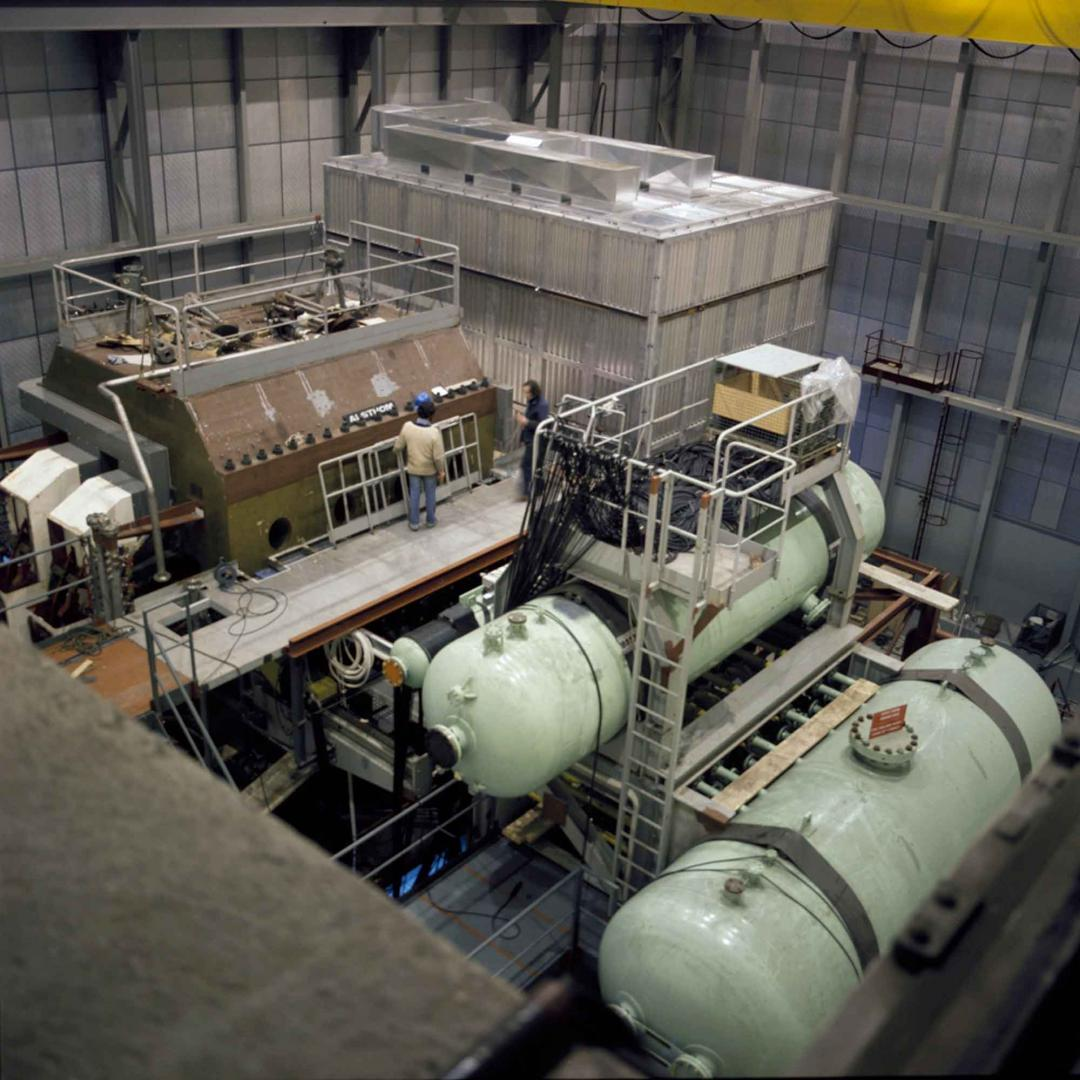
\includegraphics[width=\marginparwidth]{SM/gargamelle.jpg}
	\captionof{figure}{Gargamelle.}
	\label{GARGAMELLE}
}
\marginpar
{
	\centering
	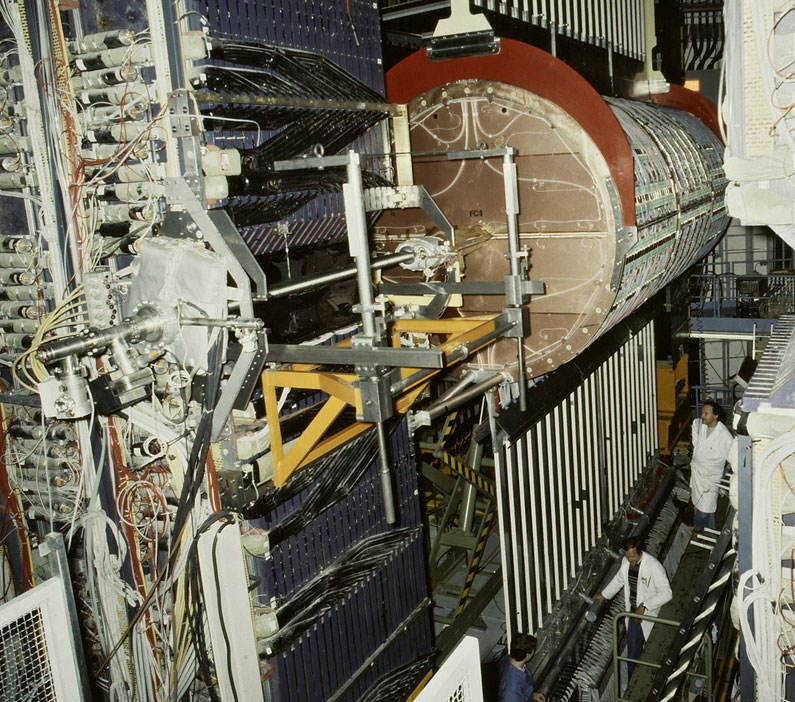
\includegraphics[width=\marginparwidth]{SM/ua1.jpg}
	\captionof{figure}{UA1.}
	\label{UA1}
}
\marginpar
{
	\centering
	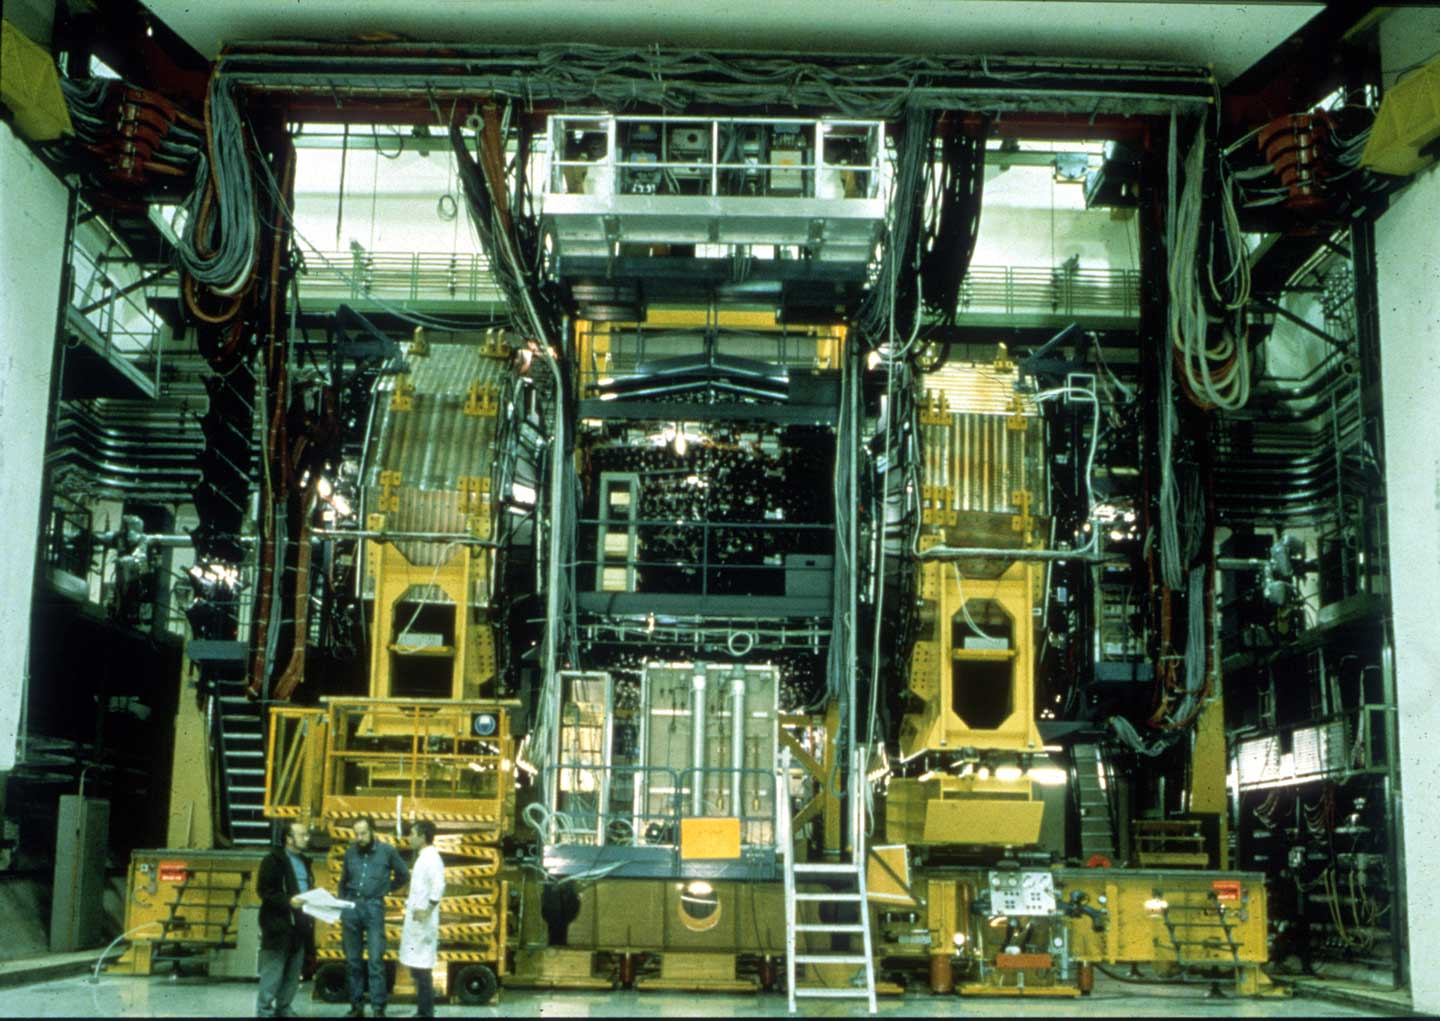
\includegraphics[width=\marginparwidth]{SM/ua2.jpg}
	\captionof{figure}{UA2.}
	\label{UA2}
}
\marginpar
{
	\centering
	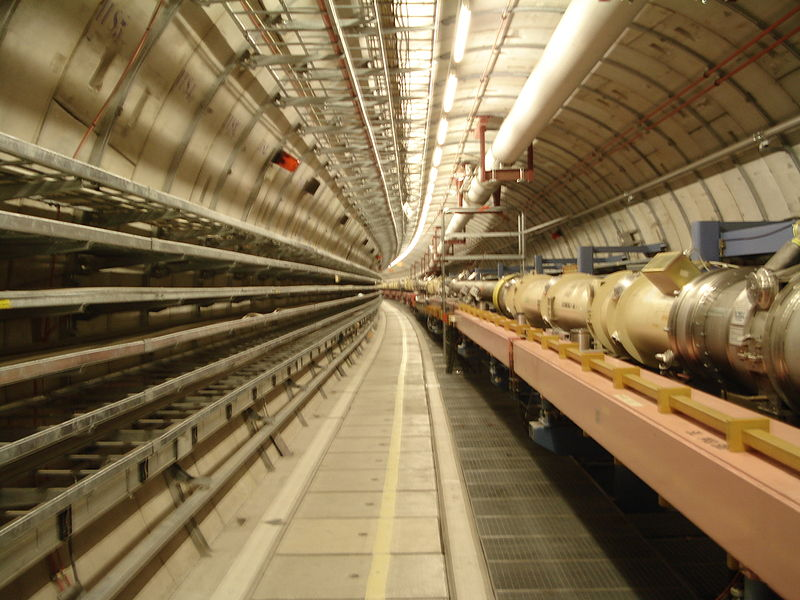
\includegraphics[width=\marginparwidth]{SM/HERA.jpg}
	\captionof{figure}{tunnel du collisionneur HERA.}
	\label{HERA}
}
\marginpar
{
	\centering
	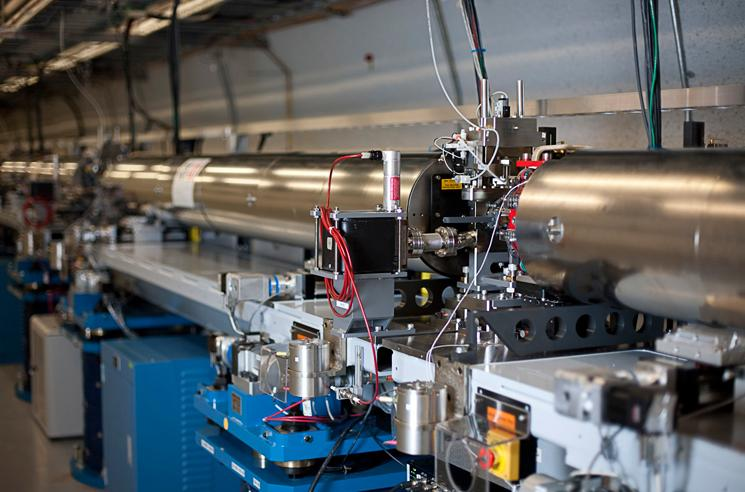
\includegraphics[width=\marginparwidth]{SM/slac.jpg}
	\captionof{figure}{Beam line du SLAC.}
	\label{SLAC}
}

De plus l'ensemble des mesures effectuées jusqu'à présent sont compatibles avec le Modèle Standard: La figure (fig.\ref{mesures}) montre la mesure de certains paramètres ainsi que leur "pull" défini par :
\begin{equation}
\frac{O^{mesure}-O^{fit}}{\sigma^{mesure}}
\end{equation}
c'est à dire la déviation entre les mesures expérimentales et les prédictions théoriques en unités de l'incertitude expérimentale. Tous les pulls sont inférieur à $3\sigma$. L'expérience et la théorie sont donc en très bon accord.

\begin{figure}[h!]
\centering
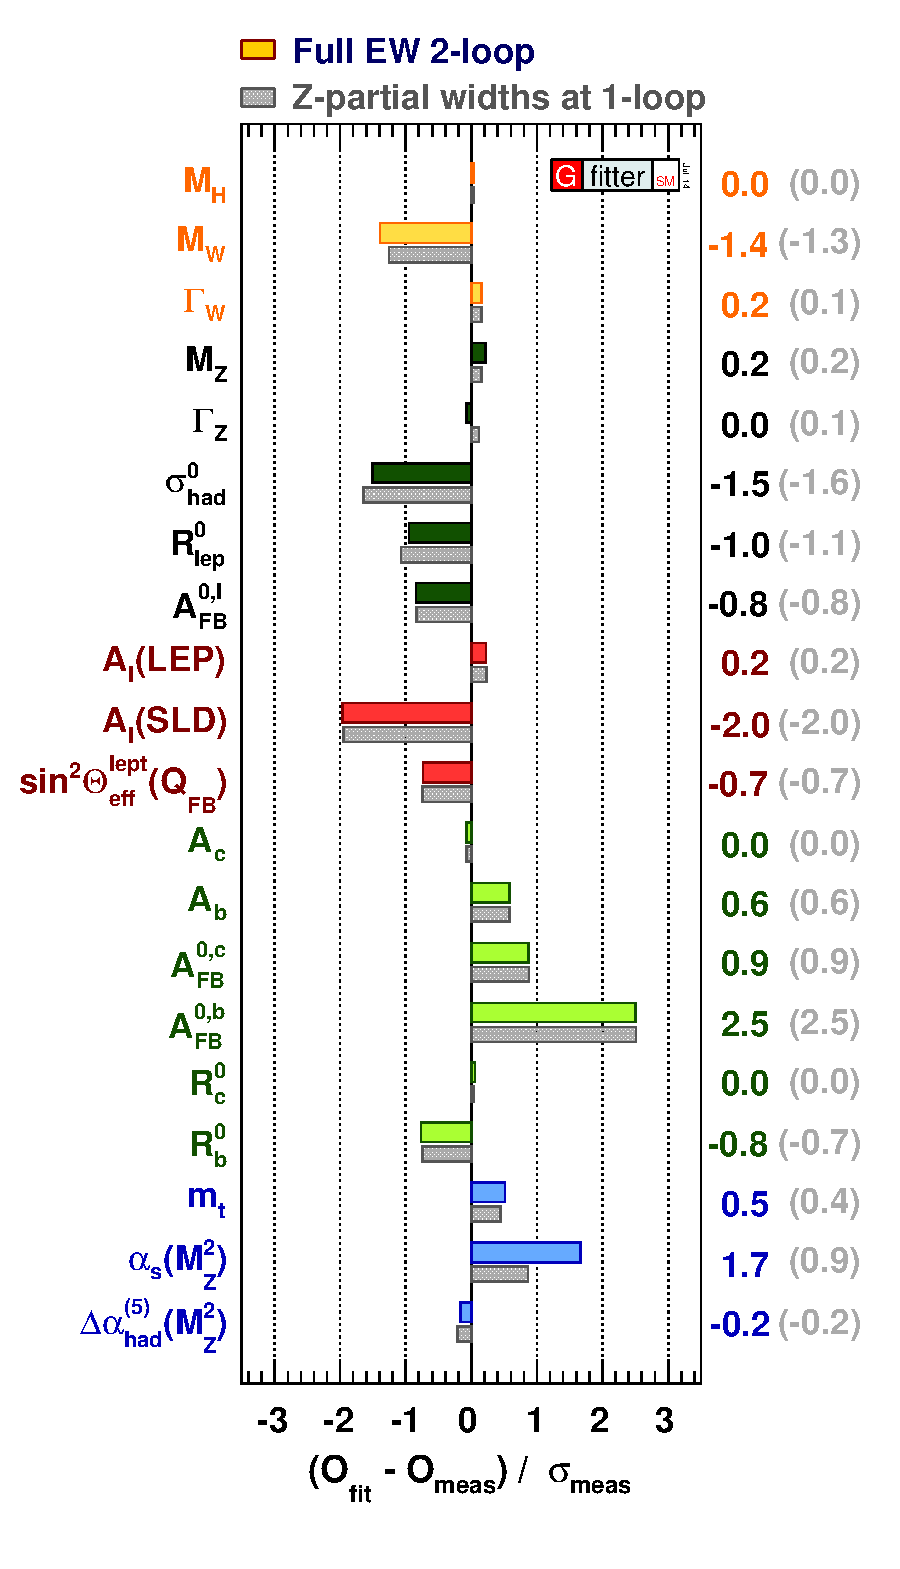
\includegraphics[width=0.50\textwidth]{SM/mesure.eps}
\captionof{figure}{Comparaison des résultats d'ajustement avec les mesures directes de certains paramètres du Modèle Standard.}
\label{mesures}
\end{figure}

\section{Les faiblesses du Modèle Standard}
Le modèle Standard est en accord remarquable avec l'expérience. Cependant, plusieurs problèmes et questions non résolubles amène à considérer le Modèle Standard comme une théorie effective, valable jusqu'à l'échelle du TeV. Une nouvelle physique qui engloberait le Modèle Standard devrait apparaitre à cette échelle d'énergie.

Parmis les principaux problèmes ou faits inexpliqués par le Modèle Standard, on peut citer :
\begin{itemize}[label=$\bullet$]
\item \textbf{Les neutrinos massifs :}
\marginpar
{
\centering
\includegraphics[width=\marginparwidth]{SM/kamiokande.jpg}
\captionof{figure}{Intérieur du détecteur Super-Kamiokande.}
\label{kamiokande}
}
\marginpar
{
\centering
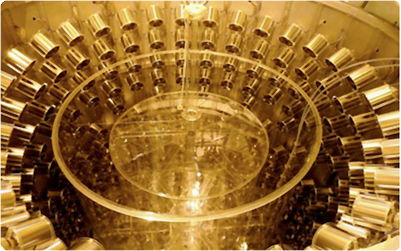
\includegraphics[width=\marginparwidth]{SM/chooz.jpg}
\captionof{figure}{Coeur du détecteur Double Chooz.}
\label{chooz}
} 
Les expérience Super-Kamiokande\ref{kamiokande} et GALLEX portant sur l'observation du flux de neutrinos provenant du Soleil et les expériences Double Chooz\ref{chooz} et K2K pour les flux de neutrinos de sources artificielles terrestres ont mis en évidence l'oscillation des neutrinos entre les saveurs leptoniques. Ces oscillations ne peuvent s'expliquer que si les neutrinos sont massifs et s'il existe des neutrinos droits. Bien que le Modèle Standard considére les neutrinos comme des particules de masse nulle et que de parité gauche, il est facile d'y ajouter un neutrino droit dans chaque famille et les couplages au doublet Higgs correspondant afin de rendre compte de ces faits expérimentaux\footnote{C'est d'ailleurs cette extension du Modèle Standard qui est présenté dans ce chapitre.}. Cependant cela aggrave le problème de la hiérarchie des masses car les masses des particules élémentaires s'étalent sur 10 ordres de grandeur !

\item \textbf{Le nombre de paramètres libres :} Le modèle standard contient 18 paramètres libres : les 3 constantes de couplages, les deux paramètres $\lambda$ et $\mu^2$ du potentiel de Higgs, 9 couplages de Yukawa et les trois angles et une phase pour les quarks dans la matrice CKM ainsi que l'angle associé auwx. Et d'autres encore en ajoutant le fait que les neutrinos soit massif.

\item \textbf{Le nombre de familles :} Le nombre de famille a été expérimentalement obtenu en comparant la section efficace hadronique en fonction de l'énergie du centre de masse expérimentale au prédiction théorique différents nombres de familles de neutrinos de masse négligeable. Actuellement on considère que trois familles\ref{neutrinos}. Cependant le fait que les neutrinos soient massif permet l'existance de plus de trois familles si les neutrinos on une masse supérieur à $m_{Z^{0}}/2$.
\begin{figure}[h!]
\centering
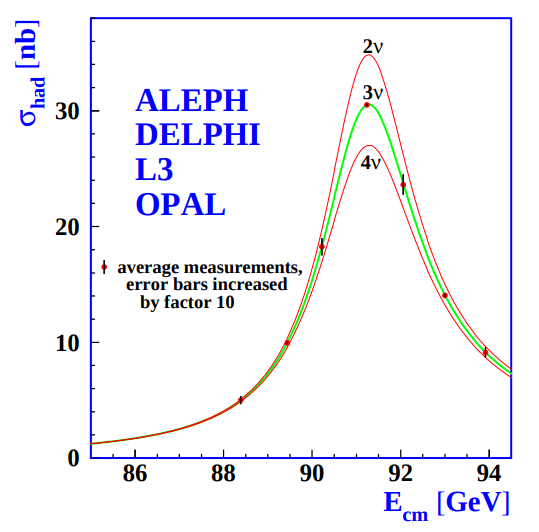
\includegraphics[width=0.48\textwidth]{SM/neutrinos.png}
\captionof{figure}{Mesures de la section efficace de production hadronique près de la résonance en Z. Les courbes indiquent les sections efficaces prédites pour deux,trois et quatres espéces de neutrinos avec les couplages du Modèle Standard et de masses négligeables.}
\label{neutrinos}
\end{figure}

\item \textbf{La baryogénèse :} Le Modèle Standard est incapable d'expliquer l'asymétrie entre la quantité de baryons (matière) et d'anti-baryons (anti-matière) observés dans l'Univers.

\item La gravitation : Le Modèle Standard ne comporte pas l'interaction gravitationnelle. Aucune formulation quantique de la gravitation n'a encore été trouvé. La meilleur théorie gravitationnelle, la relativité générale et malheureusement incompatible avec le Modèle Standard.

\item \textbf{Le problème de naturalité :} En effet, il paraît naturel de considérer une échelle d'énergie ou le Modèle Standard cesse d'être valide. Or, les ordres supérieur de la théorie perturbative ajoutent des corrections radiatives aux masses des différentes particules. En imposant une échelle d'énergie à la validité du Modèle Standard $\Lambda$, un "cut-off", les corrections vont en dépendre. Pour le boson de Higgs et en considérant les diagramme de la figure fig.\cref{corrections} on peut écrire :
\begin{equation}
m_{h}^{2}=m_{0}^{2}-\delta m_{h}^{2}
\end{equation}
avec $m_{0}^{2}$ la masse "nue" du boson, $m_{h}^{2}$ la masse effective et $\delta m_{h}^{2}$ les corrections radiative.
\begin{figure}[h!]
\centering
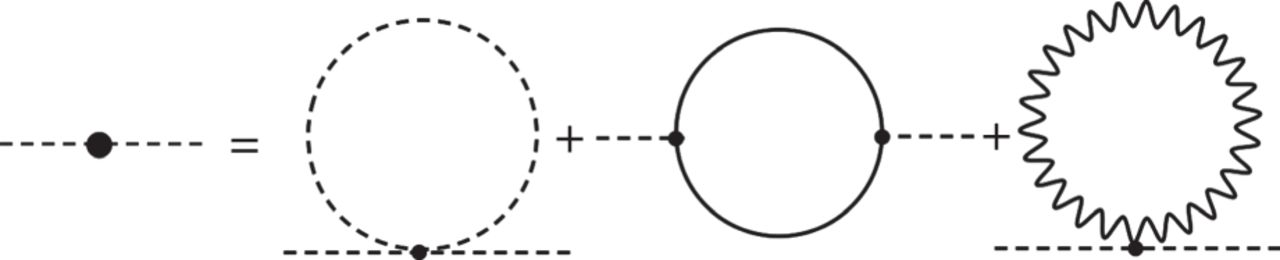
\includegraphics[width=0.40\textwidth]{SM/corrections.jpg}
\captionof{figure}{Correction radiative du premier ordre pour le boson de Higgs.}
\label{corrections}
\end{figure}
La contribution fermionique est de la forme :
\begin{equation}
\label{eq1}
\delta m_{h}^{2}=-\frac{y_{f}^{2}}{16\pi^{2}}\left(2\Lambda^{2}+6m_{f}\log\left(\frac{\Lambda}{m_{f}}\right)\cdots\right)
\end{equation}
En considérant un cut-off de l'ordre de $\Lambda \sim 10^{16}$GeV il faut donc un accord à $10^{-30}$ entre $m_{0}^{2}$ et $\delta m_{h}^{2}$. Ce problème de hiérarchie, et de réglage fin des paramètres ne semble pas naturel.

\item \textbf{La Matière Noire et l'Énergie Noire} : Des observations cosmologiques ont mis en évidence la présence de matière dite noire car elle n'émet pas et n'interagît pas avec les radiations électromagnétiques. Bien que n'ayant jamais été directement observé, son existence et certaines de ses propriétés peuvent être étudiés par leur effets gravitationnelles sur le mouvement de la matière visible, elle serait  également à l'origine de la formation des galaxies et des amas de galaxies, et de leurs répartition de façon non uniforme dans l'Univers. D'après les observations du satellite Plank\ref{Plank},
la matière que nous connaissons ne compose que 4.9\% du totale mass-énergie de l'Univers. La matière noire quant à elle ne compte que pour 26.8\%. Les 68.3\% restant sont composés d'énergie noire. Cette énergie serait responsable de l'accélération de  l'expansion de l'Univers qui à été mis en évidence en 1998 par les projets Supernova Cosmology Project et High-Z supernovae search team. Ni la matière noire ni l'énergie noire ne sont décrites par le Modèle Standard.
\marginpar
{
\centering
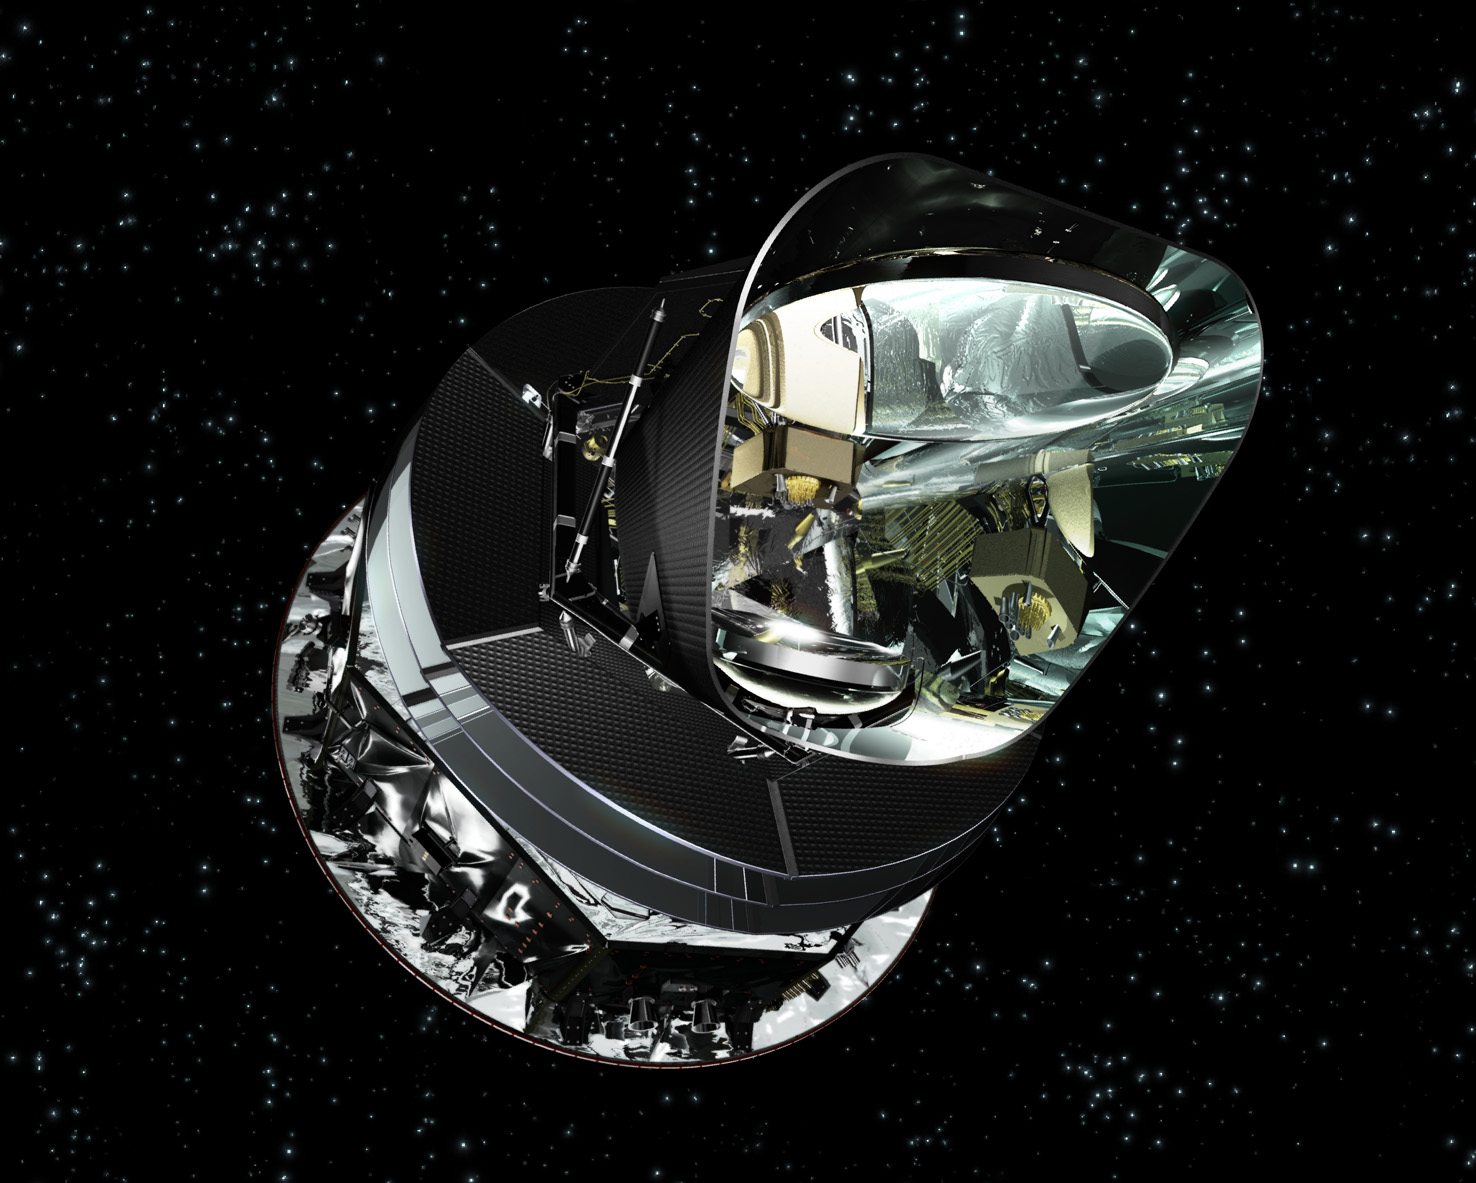
\includegraphics[width=\marginparwidth]{SM/plank.jpg}
\captionof{figure}{Le satellite Plank.}
\label{Plank}
} 

\item \textbf{La non unification des couplages : }Les constantes de couplages $\alpha_{1}$,$\alpha_{1}$ et $\alpha_{3}$ respectivement de l'interaction electromagnétique, faible et forte dépendent de l'échelle d'énergie. Il s'avére que ces trois constantes se rapprochent l'une de l'autre à haute énergie mais ne concourent pas en un seul point (cf.fig\ref{constantes}). Bien que n'étant pas en soit un problème, la convergence vers une valeur unique à haute énergie et nécessaire à une théorie "du tout" qui unifierait ces trois interactions. Le calcul de l'évolution de ces constantes par la méthode de renormalisation n'aboutissant pas à la convergence de ces trois constantes tend à prouver une lacune du Modèle Standard et son caractère effectif.
\begin{figure}[h!]
\centering
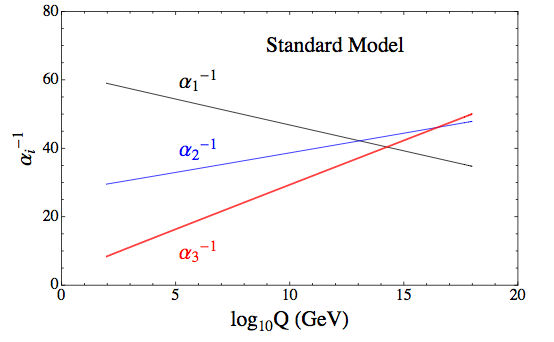
\includegraphics[width=0.50\textwidth]{SM/couplageSM.jpg}
\captionof{figure}{Évolution des constantes de couplage en fonction de l'échelle d'énergie dans le cas du Modèle Standard.}
\label{constantes}
\end{figure}
\end{itemize}

\section{Au delà du Modèle Standard}
Afin de résoudre certains de ces problèmes, de nombreux modèles théorique ont été développé, cependant aucun d'entre eux n'est capables de répondre à toutes les questions et combler les lacunes du Modèle Standard. Certaines de ces théorie sont des extensions du à ce modèle, d'autre propose des modèles complètement différents.

La majorité des modèles repose sur les symétries du Modèle Standard et cherche à les étendre : Soit en trouvant d'autres symétries internes (Grand Unified Theorries (GUT)), soit en liant les symétries internes et externes ( supersymétrie (SUSY)) voir même modifier la nature même de l'espace temps en ajoutant des dimensions supplémentaires par exemple.

\subsubsection{Les modèles de grande unification}
Ces modèles s'appuient sur le fait qu'il ait été possible de réunir dans le Modèle Standard trois des quatre interactions que nous connaissons et que leur constantes de couplage se rapprochent l'une de l'autre à haute énergie. Il semble donc logique de vouloir unir ces trois interactions sous une même symétrie. Il n'existerait alors plus qu'un groupe G et qu'une seule constante de couplage. Ces théories doivent bien sûr être renormalisables et leur groupe doit avoir comme sous groupe celui du Modèle Standard $SU(3)\otimes SU(2) \otimes U(1)$. Les groupes $SU(5)$ et $SO(10)$ ont notamment été étudié.

\subsubsection{Modèles à dimensions supplémentaires}
Ces modèles tentent de supprimer la naturalité et la hiérarchie des échelles d'énergies en faisant tendre l'échelle de Planck vers celle de l'interaction faible. Pour cela ils prennent comme hypothèse que l'espace temps contient des dimensions supplémentaires enroulées compacts. L'interaction gravitationnelle évolue donc dans ces dimension supplémentaires.

\subsubsection{La supersymètrie}
La supersymètrie a été introduite par Weiss et Zumino en 1974. Elle consiste à supprimer les divergences quadratiques  en les annulant grâce à l'ajout de termes supplémentaires. Pour cela on associe à chacun des fermions $f_{L}$ et $f_{R}$ un partenaire scalaire $\tilde{f}_{L}$ et $\tilde{f}_{R}$ possédant les mêmes nombres leptoniques et baryoniques. Ces partenaires contribuent donc aux diagramme de correction radiative de la masse du Higgs (cf.fig\ref{corrections}). Les boucles scalaires ont une contribution positive contrairement aux boucles fermioniques, il est ainsi possible de supprimer le terme en $\Lambda^2$ de la formule (\ref{eq1}). La masse du Higgs est varie alors comme le logarithme de l'énergie $\Lambda$. On supprime ainsi le problème du fine-tuning et de la naturalité. Les équations de renormalisation sont également modifiées et il est possible de faire concourir les constantes de couplages en un point. La supersymètrie est donc également un candidat à une théori du "tout". La supersymètrie souffre cependant de certains problèmes, en effet, les particules superpartenaires sont censé être de même masse que les particules élémentaires. Or aucune superparticule n'a encore été detécté expérimentalement. Il faut donc introduire un mécanisme de brisure de la supersymètrie.

Nombres de ces théories postulent l'existence de nouvelles particules ou d'effets qui peuvent être vérifier expérimentalement. Pour pouvoir savoir laquelle de ces théories décrit au mieux la la nature ou contraindre ces modèles, il est nécessaire de construire de nouveaux accélérateurs toujours plus puissant et des détecteurs de plus en plus perfectionnés. 

\chapter{Le Grand collisionneur de hadrons (LHC)}
\renewcommand\chapterillustration{LHC/lhc}
\ThisULCornerWallPaper{1}{\chapterillustration}
\minitoc
\lettrine[lines=4, slope=-0.5em]{C}{e} chapitre décrit le complexe des accélérateurs du CERN\footnote{Organisation Européenne pour le Recherche Nucléaire (Laboratoire européen de physique des particules)} qui permet d'accélérer les particules, afin d'avoir un faisceau de particules avec une énergie suffisante pour être injecté dans le Grand Collisionneur de Hadrons (LHC\footnote{Large Hadron Collider}) et atteindre une énergie finale de $7$ TeV. Cette description bien que succincte est nécessaire car de nombreux résultats obtenus durant cette thèse ont nécessité l'utilisation d'accélérateurs de ce complexe. Une description du LHC est également donnée, car ses performances présentes et futures déterminent les choix technologiques des détecteurs utilisant son faisceau.

\section{Le complexe d'accélérateurs du CERN}

Le complexe d'accélération (\ref{complexe}) du CERN est une série de machines qui délivrent des faisceaux de particules d'énergies de plus en plus élevées. Chaque machine accélère les faisceaux et les injecte dans la machine suivante. Le dernier accélérateur du complexe est le LHC.

Le programme de ce dernier est surtout basé sur des collisions protons-protons. Cependant chaque année, environ un mois est consacré aux collisions d'ions lourds (plomb-plomb) ou (proton-plomb) afin d'étudier notamment le plasma de quarks et gluons, l'une des phases de l'Univers peu après le Big Bang. 

Dans le cas de ces collisions, la chaine d'accélération est constituée du Linear Accelerator 3 (LINAC 3), du Low Energy Ion Ring (LEIR) utilisé pour le stockage des ions et leur refroidissement. La chaine d'accélération est ensuite identique à celle pour les collisions proton-proton.

\begin{minipagewithmarginpars}[h]{\textwidth}
  	\centering
	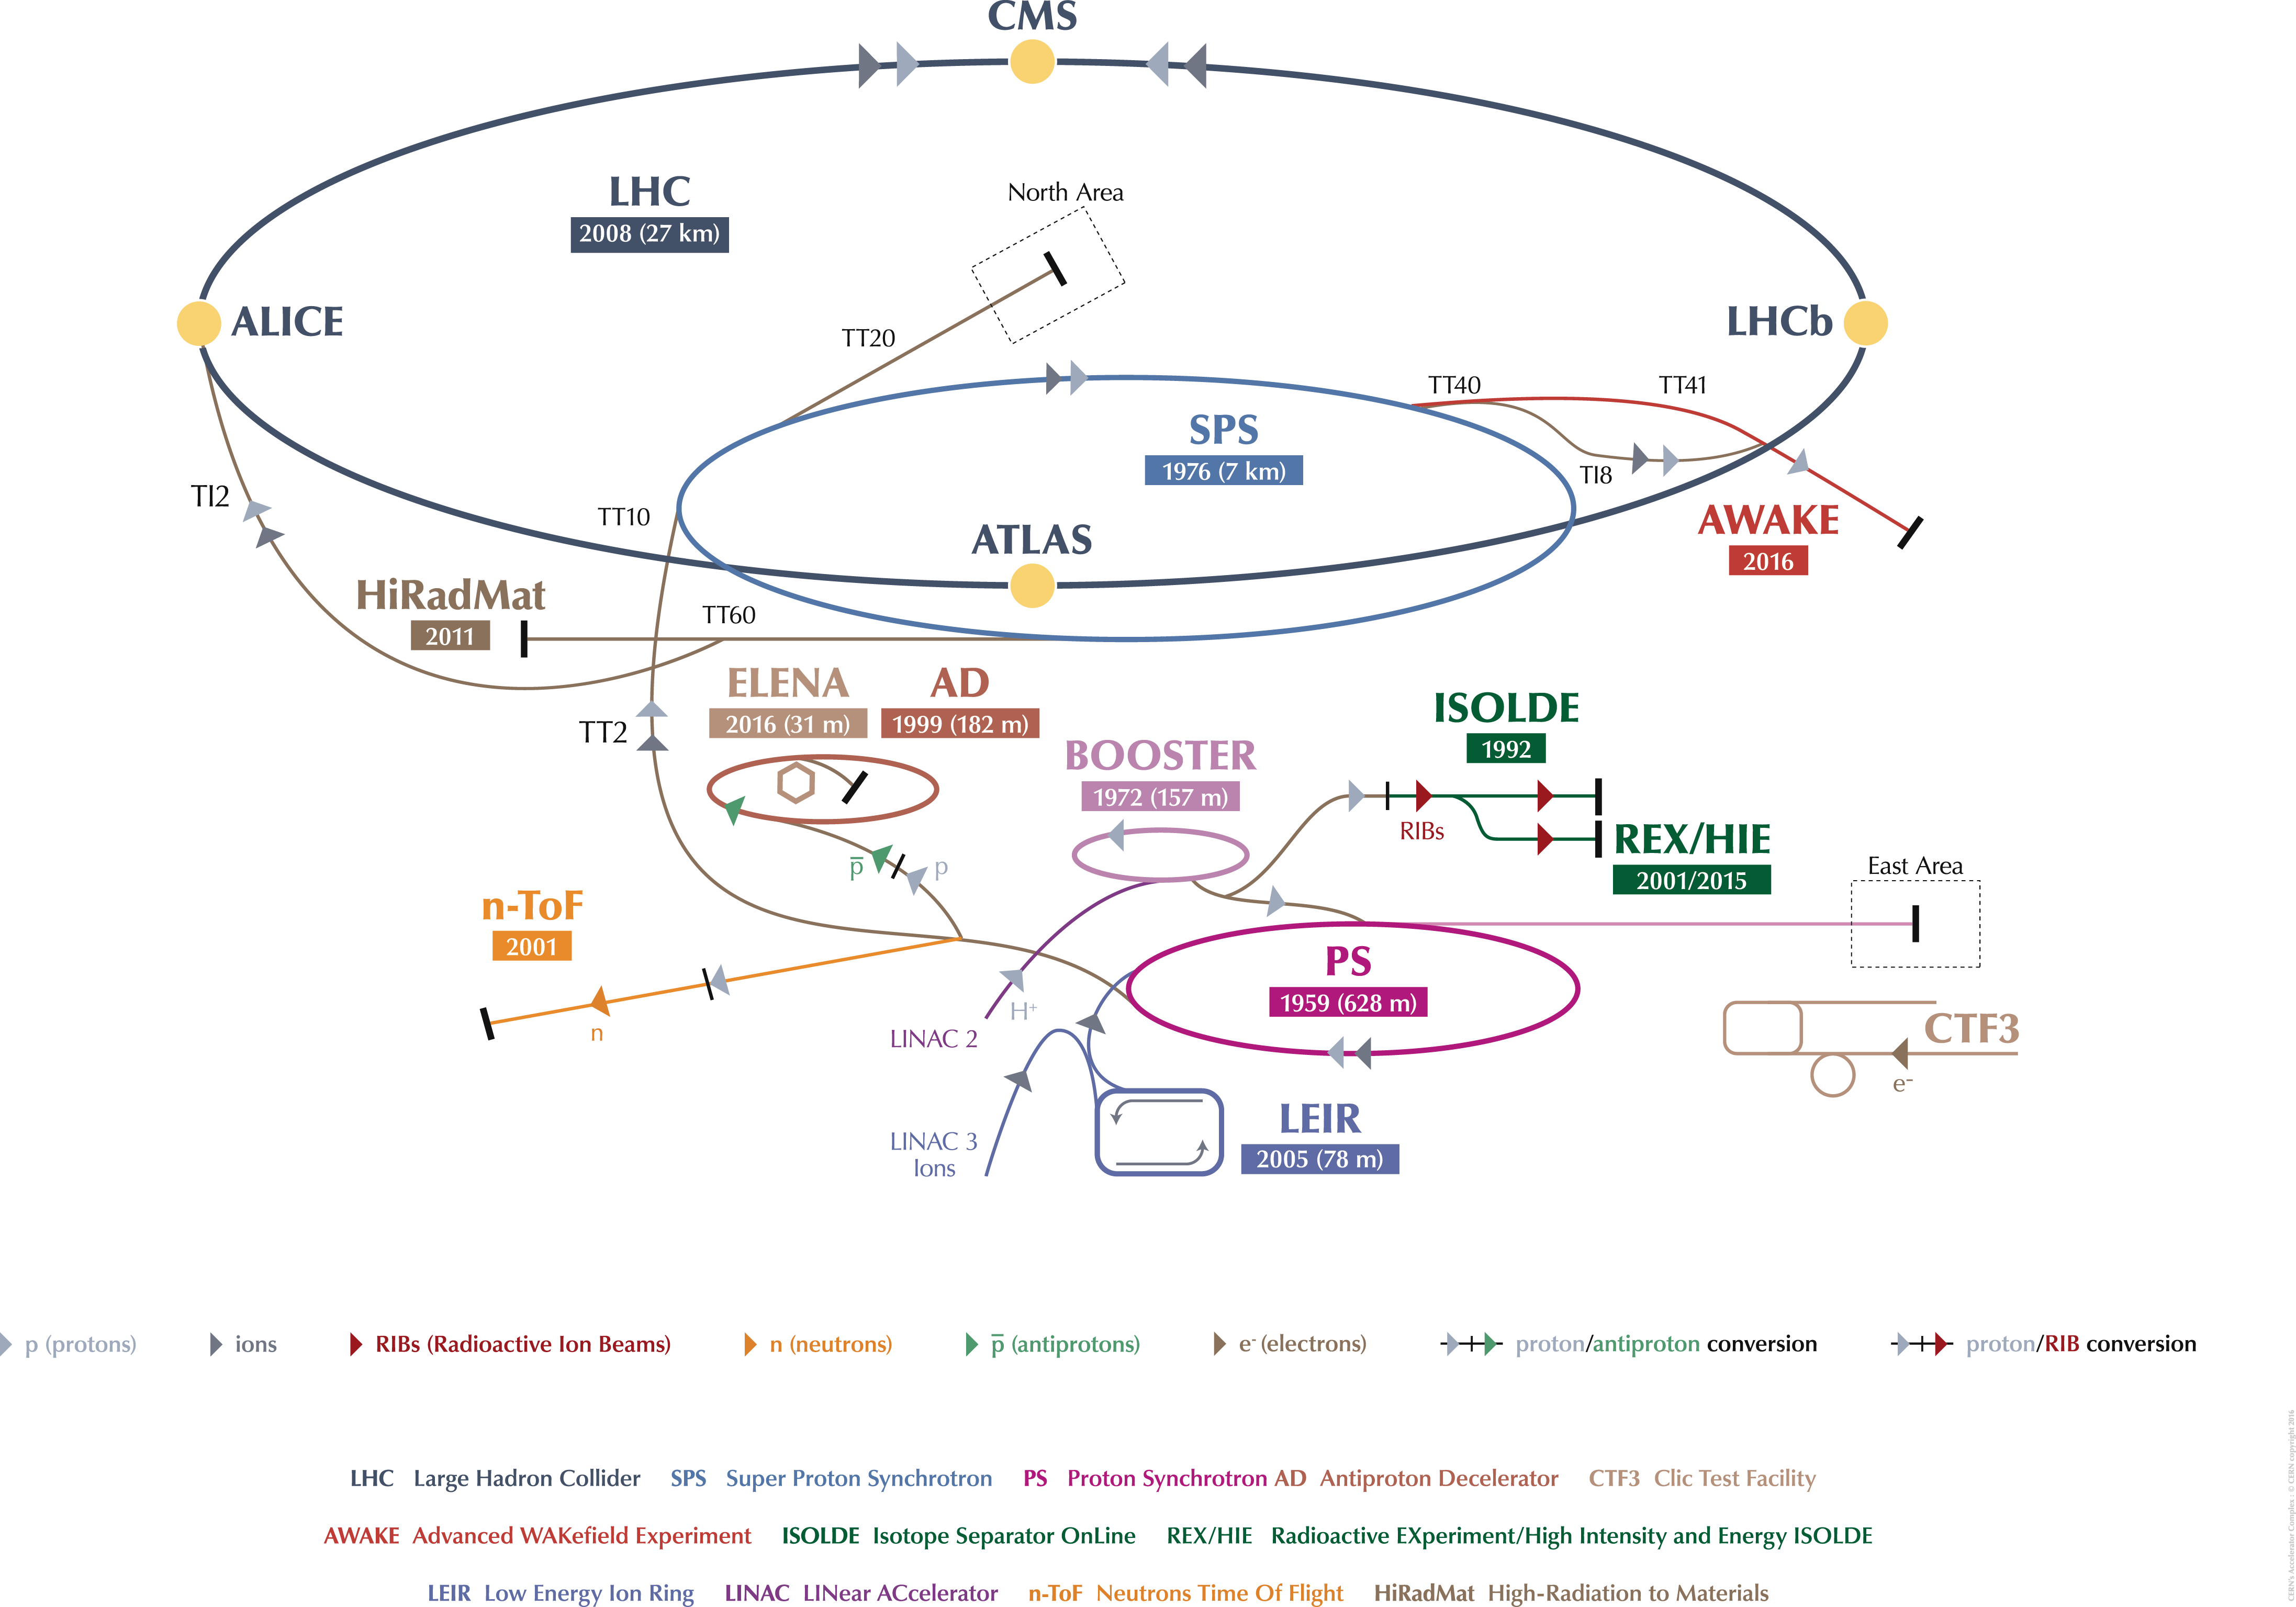
\includegraphics[scale=0.25]{LHC/complexe.png}
  	\captionof{figure}{Schéma du complexe d'accélération du CERN. La chaine d'injection du LHC est constituée du Linac 2, du Booster, du PS et du SPS}
  	\label{complexe}
  	\par 	
\marginpar
{
	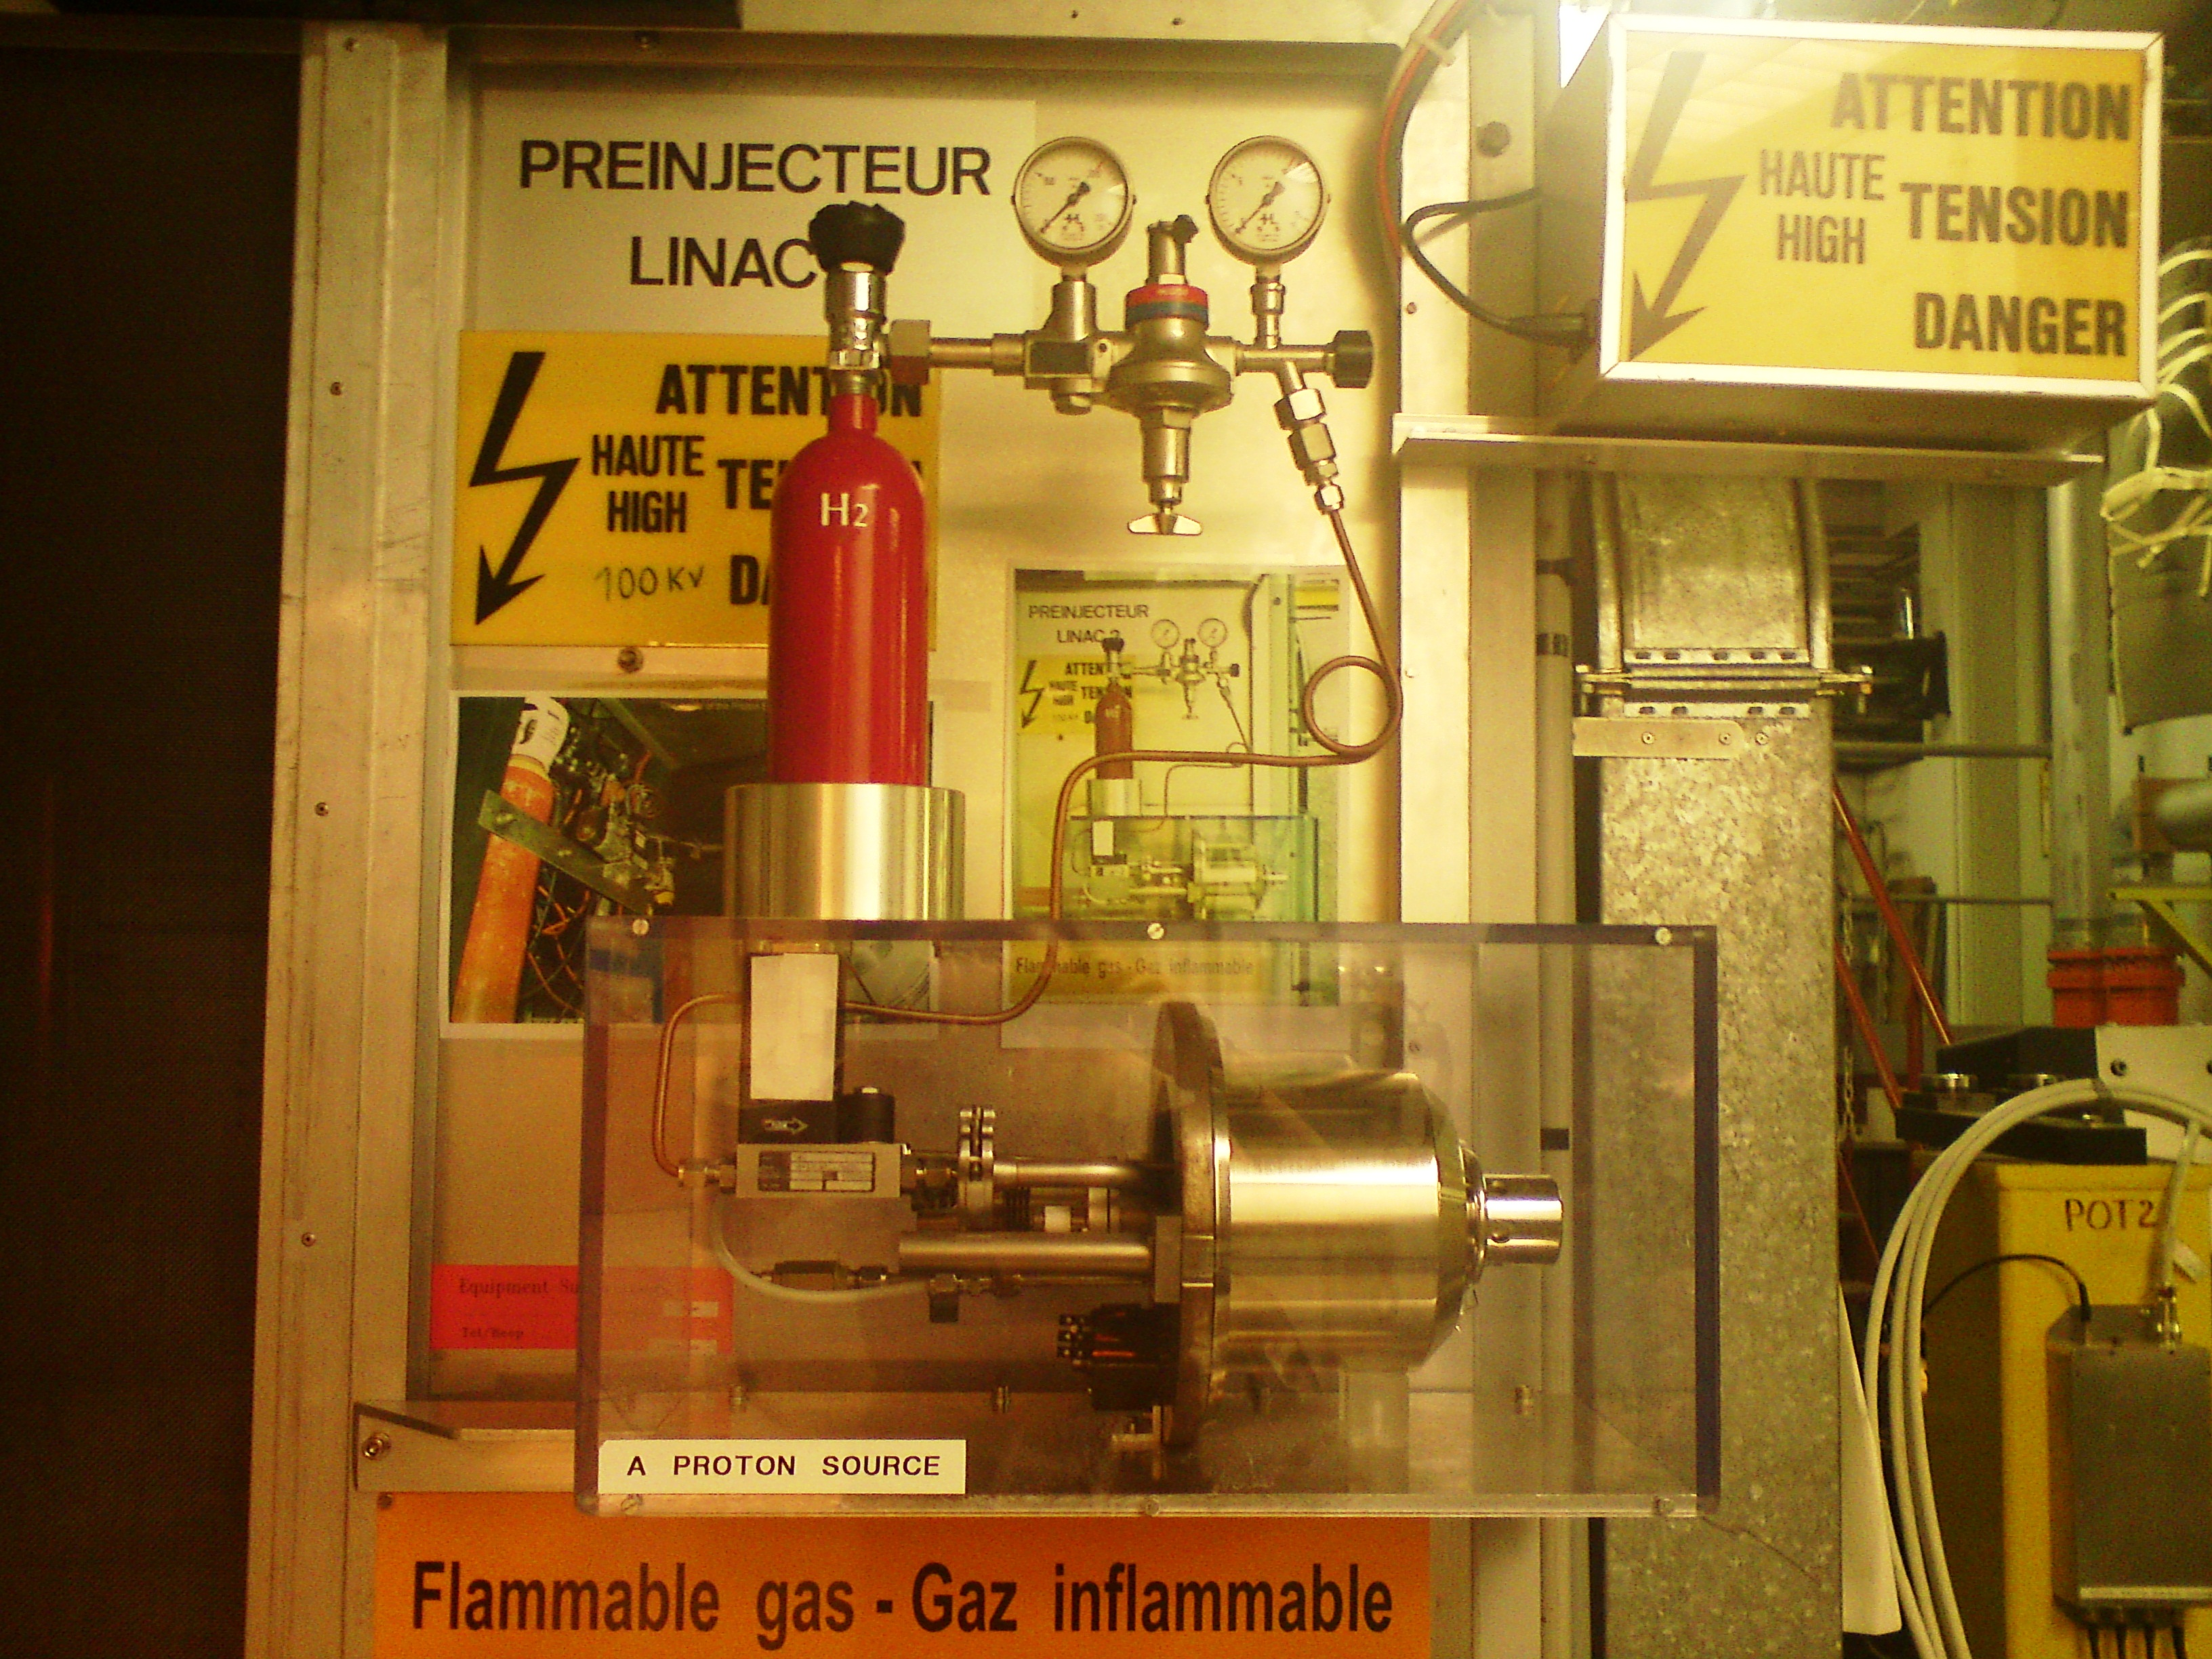
\includegraphics[width=\marginparwidth]{LHC/Bouteille.jpg}
	\label{bouteille}
    	\captionof{figure}{Source des protons du LHC.}
}	
\end{minipagewithmarginpars}

\marginpar
{
	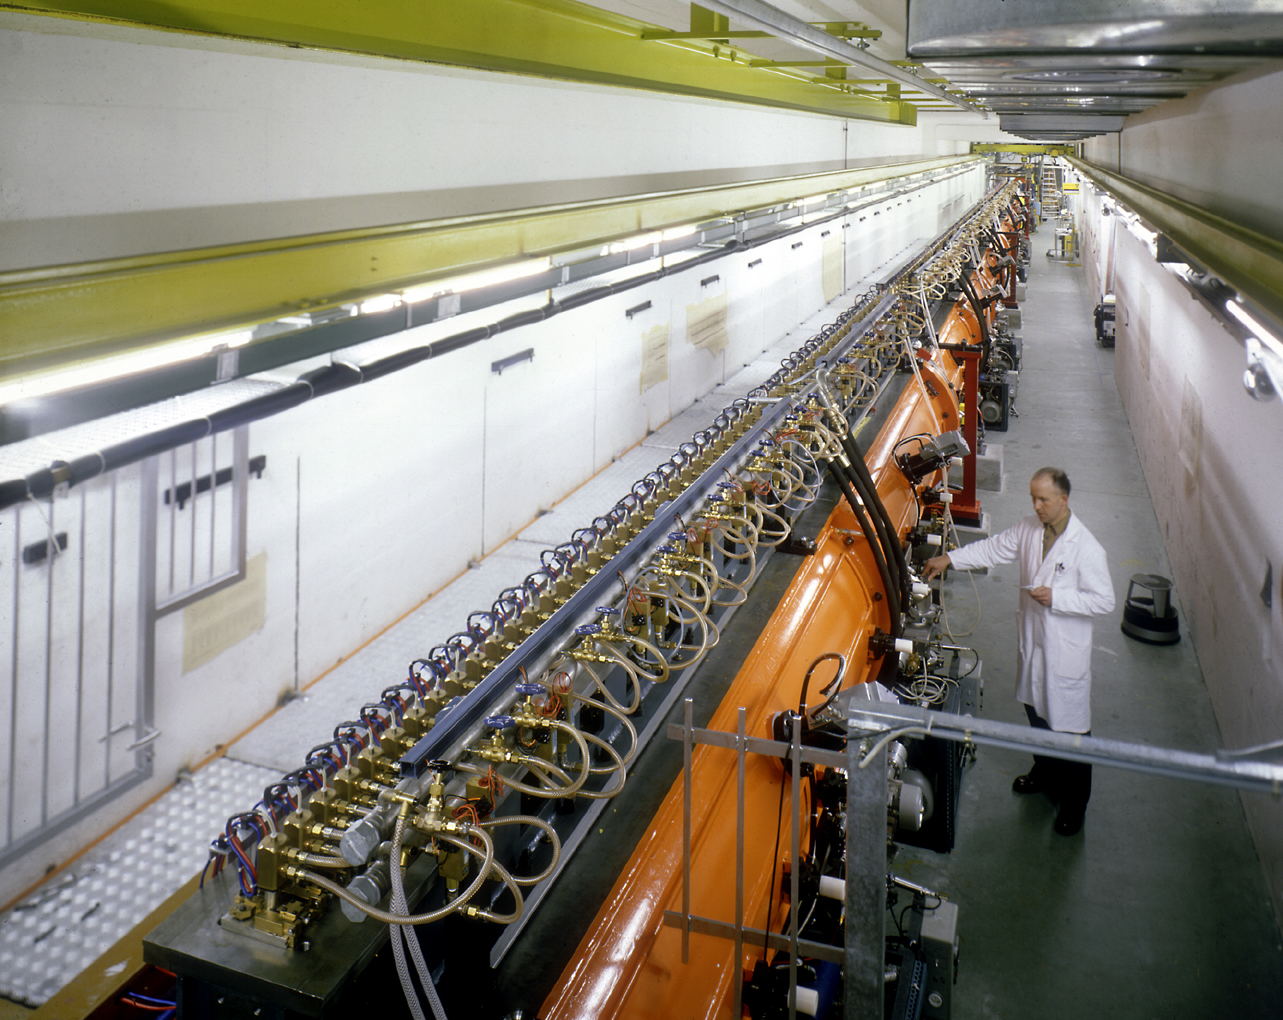
\includegraphics[width=\marginparwidth]{LHC/linac2.jpg}
    \captionof{figure}{Photo du LINAC 2.}
    	\label{linac2}
}

\marginpar
{
	
	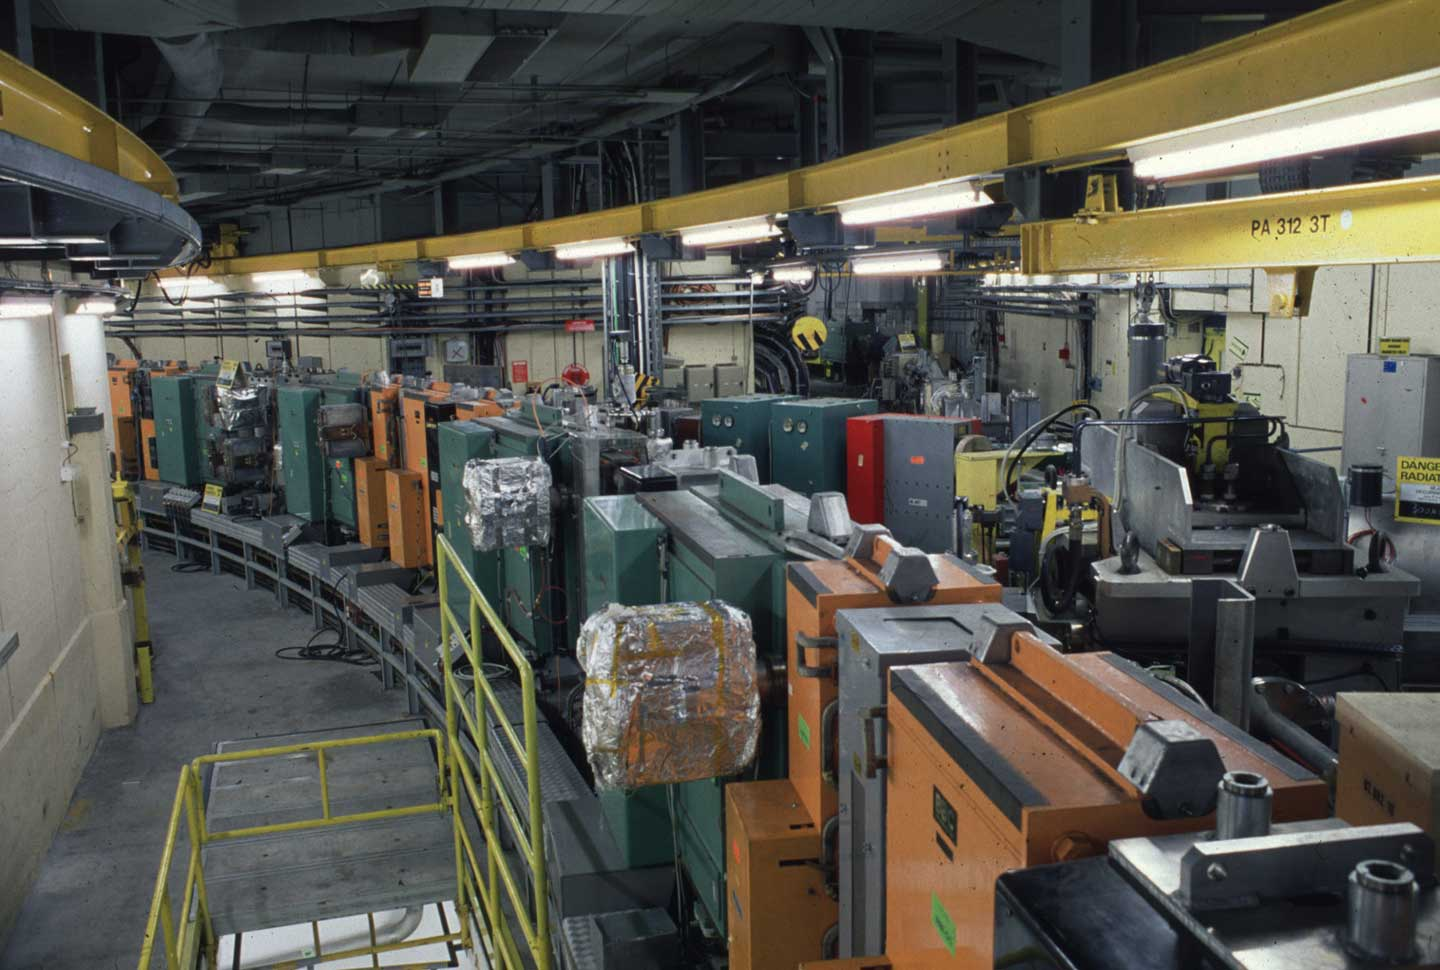
\includegraphics[width=\marginparwidth]{LHC/booster.jpg}
    \captionof{figure}{Photo du Booster du Synchrotron à protons.}
    	\label{booster}
}

\marginpar
{
	
	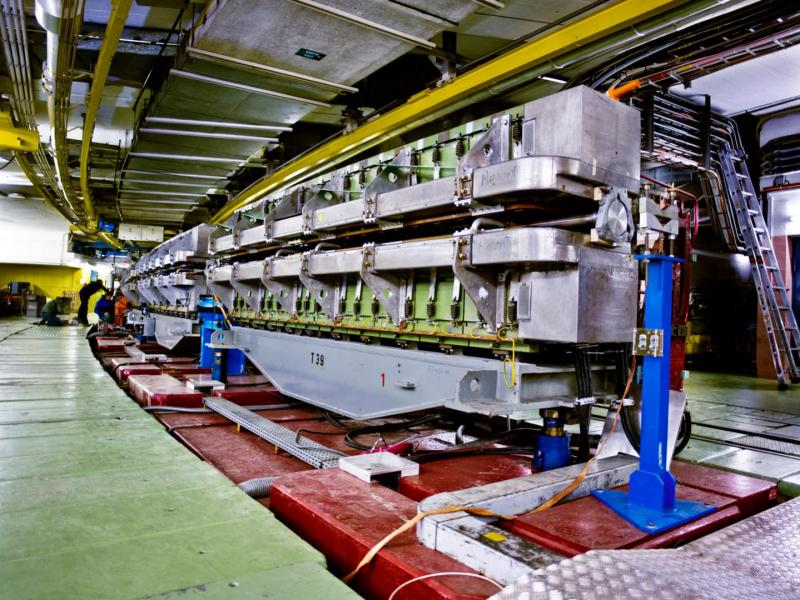
\includegraphics[width=\marginparwidth]{LHC/ps.jpg}
    \captionof{figure}{Photo du PS.}
    	\label{ps}
}

\marginpar
{
	
	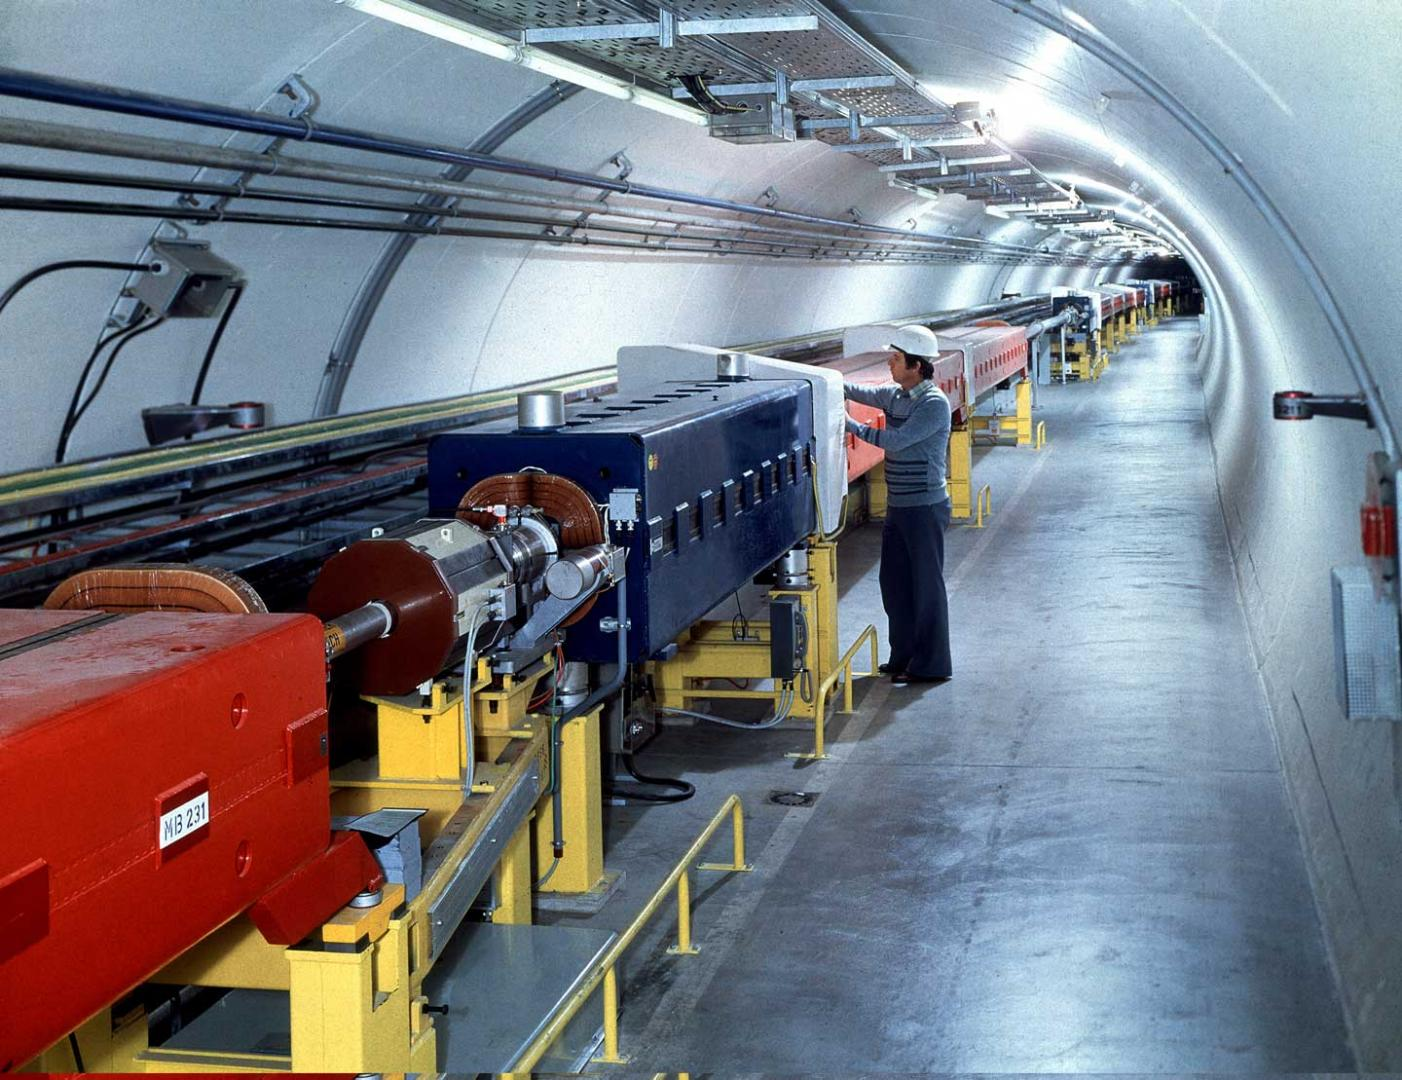
\includegraphics[width=\marginparwidth]{LHC/sps.jpg}
    \captionof{figure}{Photo du SPS.}
    	\label{sps}
}
Pour les collisions proton-proton, la source de protons est une bouteille de dihydrogène gazeux (fig. \ref{bouteille}). Les atomes d’hydrogène sont soumis à un champ électrique, qui arrache leurs électrons et les ionise en $H^{+}$ (proton). Les protons extraits sont ensuite envoyés dans l'accélérateur linaire (LINAC 2 (fig. \ref{linac2})) où ils atteignent l'énergie de 50 MeV et sont $5\%$ plus massifs. Ils passent ensuite dans les 4 anneaux de 157m de circonférence du Booster du Synchrotron à protons (BOOSTER (fig. \ref{booster})) qui les amènent à une énergie de 1.4 GeV avant de les injecter dans l'accélérateur suivant, le Synchrotron à protons (PS (fig. \ref{ps})). Cet accélérateur circulaire de 628 mètres de circonférence, permet aux faisceaux d'atteindre une énergie de 25 GeV. Il sert aussi à préparer le faisceau en le découpant en série de paquets (bunchs) de particules nécessaires au LHC. Ces bunchs sont ensuite envoyés dans le supersynchrotron à protons (SPS (fig. \ref{sps})) d'une circonférence de 7 km, où l'énergie du faisceau atteint 450 GeV. Les paquets sont regroupés pour former des trains de paquets avant d'être enfin envoyés dans le Grand Collisionneur de Protons (LHC). L'injection et le guidage de faisceaux d'une telle énergie par des aimants supraconducteurs rapides est une tâche délicate et pourrait détériorer l'accélérateur. Un faisceau de test de faible intensité "pilot beam" est donc injecté afin de mesurer et vérifier les paramètres. Le faisceau de haute énergie est ensuite séparé en deux et injecté dans deux conduits différents, l'un circulant dans un sens et l'autre dans le sens contraire. Ces faisceaux sont ensuite accélérés jusqu'à une énergie de 7 TeV et ne se croisent qu'aux points d'intéractions.

\section{Le Large Hadron Collider}
Le LHC est le dernier accélérateur circulaire du complexe d'accélération. Il utilise le tunnel de 27 km de circonférence situé à une centaine de mètres sous terre. Il fût construit pour acceuillir le Grand collisionneur électron-positron (LEP\footnote{Large Electron Positron collider.}), qui fût en service de 1989 à 2000. Le LHC à été mis en service en 2008 et a été construit afin de produire de l'ordre de 600 millions de collisions proton-proton par seconde à une énergie au centre de masse de $\sqrt{s}=14$ TeV. Il est actuellement l'accélérateur de proton-proton le plus puissant du monde, et a permis de mettre en évidence l'existence du boson de Higgs, dernière pièce manquante du Modèle Standard.

Le LHC est un collissioneur de particules non fondamentales (hadrons) à l'inverse de son prédécesseur, le LEP qui utilisé des électrons et des positrons. Lors d'une collission entre hadrons, ceux sont ses constituant élementaires, les quarks et les gluons qui collissionnent entre eux. Ceux-ci possèdent seulement une portion de l'énergie du hadrons qui les contient. L'énergie du centre de masse de cette collision n'est donc pas connue avec précision. Le LHC est donc une machine de découverte de particules plutôt qu'une machine de mesures de précisions comme l'était le LEP, car il permet d'acceder à un large spectre en énergie. Généralement, les mesures de précision sont effectué grâce à des collisionneur utilisant des particules élémentaires ($e^{-}$,$e^{+}$); ils sont dans ce cas souvent linéaire afin d'éviter la perte d'énergie par rayonnement synchroton.

La figure \ref{lhcschema} est une vue schématique du LHC. En vérité le LHC n'est pas parfaitement circulaire, mais est composé de $8$ octants composés d'une section droite de longueur $~5$ km et d'un secteur courbe d'une longueur de $~3$ km (fig. \ref{octants}). Les sections droites sont utilisées afin de faire collisionner les deux faisceaux de protons venant en sens inverse l'un de l'autre. Il existe $8$ points potentiels d'interactions (P), mais seulement $4$ sont le siège de collisions et possèdent des détecteurs qui analysent les données issues de ces collisions : le point P1 pour ATLAS\footnote{A Toroidal LHC ApparatuS, détecteur généraliste.}, le point P2 pour ALICE\footnote{A Large Ion Collider Experiment, dédié à l'étude du plasma de quarks et gluons.}, le point P5 pour CMS\footnote{Compact Muon Solenoid, détecteur généraliste.} et le point P8 pour LHCb\footnote{Large Hadron Collider beauty experiment, dédié au quark b.}.

\begin{minipagewithmarginpars}[h]{\textwidth}
  	\centering
	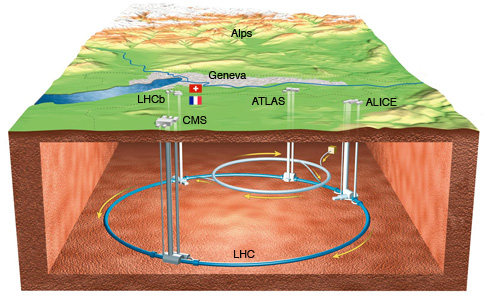
\includegraphics[scale=0.6]{LHC/CERNMap.jpg}
  	\captionof{figure}{Vue schématique du LHC.}
  	\label{lhcschema}
  	\par 	
\marginpar
{
	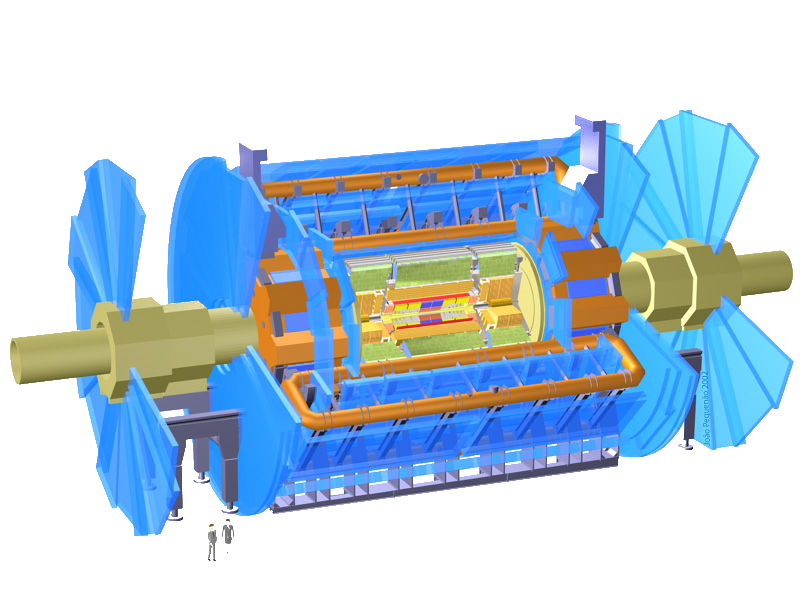
\includegraphics[width=\marginparwidth]{LHC/atlas.png}
    \captionof{figure}{ATLAS.}
    	\label{atlas}
}
\end{minipagewithmarginpars}

\begin{minipagewithmarginpars}[h]{0.95\textwidth}
  	\centering
	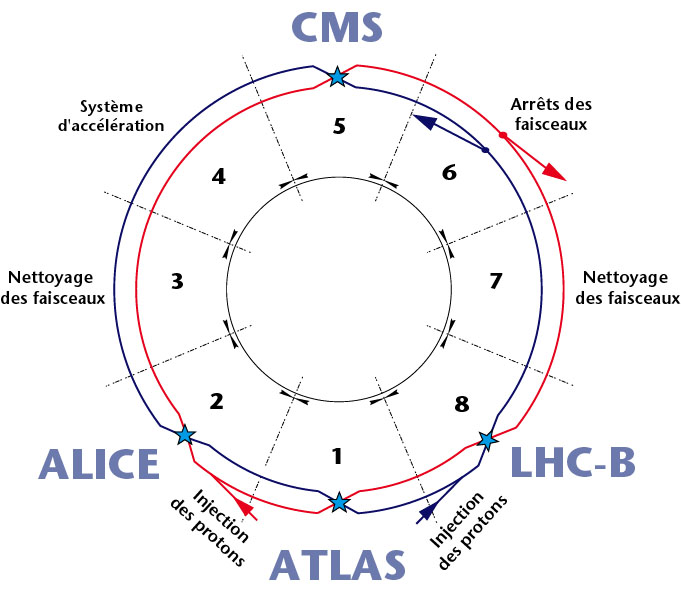
\includegraphics[width=0.55\textwidth]{LHC/lhc-schematic.jpg}
  	\captionof{figure}{Vue schématique des octants du LHC ainsi que des positions des principaux détecteurs le long du LHC. Les faisceaux (en bleu et rouge) circulent en sens inverse l'un de l'autre.}
  	\label{octants}	
  	\par 	
\marginpar
{
    \vspace*{-7.5cm}
	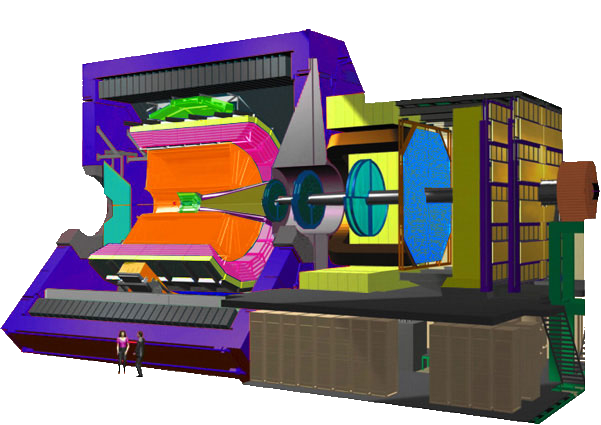
\includegraphics[width=\marginparwidth]{LHC/alice.png}
    \captionof{figure}{ALICE.}
    	\label{alice}
}
\end{minipagewithmarginpars}
\marginpar
{
	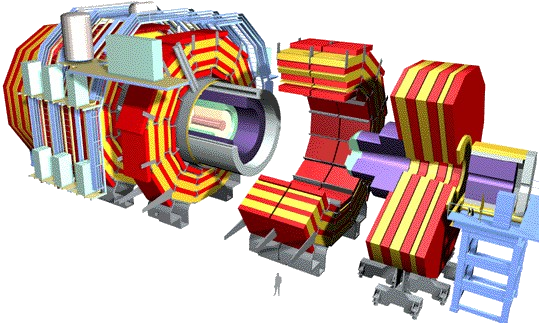
\includegraphics[width=\marginparwidth]{LHC/cms.png}
    \captionof{figure}{CMS.}
    	\label{cms}
}
\marginpar
{
	
	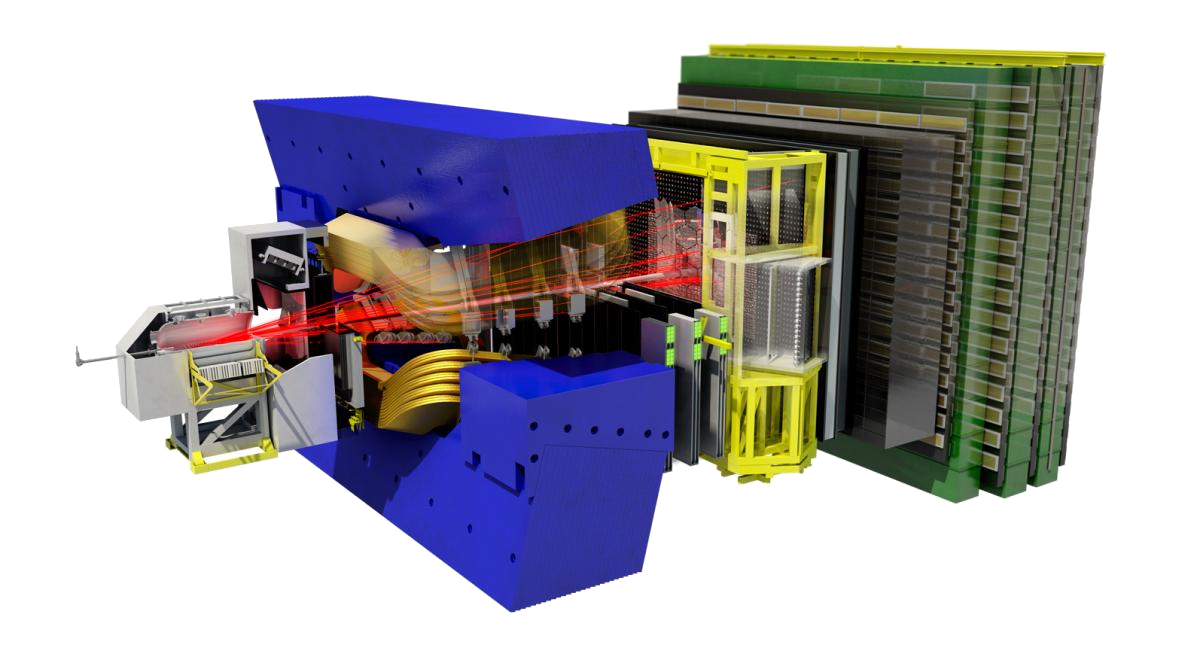
\includegraphics[width=\marginparwidth]{LHC/lhcb.png}
    \captionof{figure}{LHCb.}
    	\label{lhcb}
}

\section{Luminosité des faisceaux}
\chapter{Le détecteur Compact Muon Solenoid (CMS)}
\renewcommand\chapterillustration{CMS/cms.jpeg}
\ThisULCornerWallPaper{1}{\chapterillustration}
\minitoc

\lettrine[lines=4, slope=-0.5em]{C}{e} chapitre décrit le détecteur CMS et les sous-détecteurs qui le compose, suivi d'une discussion sur le système de déclenchement. Il décrit également certaines des mises à niveau qui se dérouleront durant les \textit{Long Shut Down} LS2 et LS3 afin de se préparer à l'augmentation de la luminosité et de l'empilement qui en découle.

\section{Le détecteur Solénoïde compact à muons (CMS)}
Le détecteur Solénoïde Compact à Muons abrégé en CMS (pour \textit{Compact Muon Solenoid}) est avec ATLAS une expérience généraliste qui a comme buts majeurs :

\begin{itemize}[label=$\bullet$]
	\item \textbf{La recherche du boson de Higgs : } Lors de la conception de CMS dans les années \num{1990}, la détection du boson de Higgs a été prise comme référence afin de tester les performances du design du détecteur. Ce but a été réalisé avec la découverte d'une particule compatible avec le boson de Higgs le \num{4} juillet \num{2012}.
	\item \textbf{Confirmer et préciser les mesures de la physique du Modèle Standard : } Des mesures de précisions dans des domaines tels que la QCD, le couplage électrofaible, et la physique des saveurs pourraient donner des indications d'une physique au-delà du Modèle Standard.
	\item \textbf{La recherche de signes de physique au-delà du Modèle Standard : }CMS permet la recherche de particules supersymétriques ou de nouveaux bosons vecteurs massifs ($Z'$) ou encore la recherche de dimensions supplémentaires par exemple.
	\item \textbf{Étudier les collisions d'ions lourds.}
\end{itemize}

Afin de répondre à ces objectifs, le "\textit{Technical Design Report}" (TDR) \cite{Bayatian:922757} a fixé le cahier des charges et les caractéristiques essentielles du détecteur CMS, à savoir :
\begin{itemize}[label=$\bullet$]
	\item Une bonne identification des muons et une bonne résolution en impulsion sur une vaste gamme d'impulsion pour la région $|\eta|<$\num{2.5}, une bonne résolution en masse pour les dimuons ($\approx$ \num{1}\% à \SI{100}{\giga\eV/\square\c}) et la capacité à déterminer de manière certaine la charge des muons d'impulsion $p<$ \SI{1}{\tera\eV/\c}.
	\item Une bonne résolution en impulsion pour les particules chargées ainsi qu'une bonne efficacité de reconstruction dans le trajectographe interne (\textit{inner tracker}). Un déclenchement et un étiquetage efficace pour les jets venant de quarks $\tau$ et $b$, ce qui requiert un détecteur à pixels proche du point d'interaction.
	\item Une bonne résolution pour l'énergie électromagnétique, et une bonne résolution en masse pour les diphotons et diélectrons  ($\approx$ \num{1}\% à \SI{100}{\giga\eV/\square\c}), une grande couverture géométrique ($|\eta|<2.5$), une mesure de la direction des photons et/ou une localisation correcte du vertex primaire d'interaction ainsi qu'une bon rejet des $\pi_{0}$ et une isolation des photons et leptons efficace à haute luminosité.
	\item une bonne résolution en masse des dijets et une bonne résolution en masse de l'énergie transverse manquante $E_{T}^{miss}$. Ceci requiert un calorimètre hadronique hermétique de très grande couverture géométrique ($|\eta|<5$) et une fine segmentation latérale ($\Delta\eta\times\Delta\phi<0.1\times0.1$)
\end{itemize} 

\subsection{Systèmes de coordonnées conventionnels}
Le système de coordonnées utilisé dans CMS est un repère cartésien $\left(O,\vec{x},\vec{y},\vec{z}\right)$ où $O$ est l'origine du repère et coïncide avec le point nominal d'interaction (IP) qui est le centre du détecteur. Le système de coordonnées est déterminé par l'axe $z$ qui est défini comme étant parallèle et dans la même direction que le faisceau allant dans le sens anti-horaire vue de dessus. L'axe $x$ pointe vers le centre du collisionneur LHC. L'axe $y$ est orthogonal au plan $xz$ et pointe vers le haut. CMS possédant une symétrie cylindrique, le repère $\left(O,\vec{r},\vec{\phi},\vec{z}\right)$ est souvent utilisé. $z$ correspond à la distance entre le plan perpendiculaire à l'axe du faisceau (appelé plan transverse) passant par le point considéré et l'origine $O$ du repère; $\phi$ est mesuré par rapport à l'axe $\vec{x}$ dans le plan $xy$ (angle d'émission par rapport à l'axe du faisceau) et $r=\sqrt{x^2+y^2}$. L'angle polaire $\theta$ est définit par rapport à $z$. Un troisième type de coordonnées, utilisant le fait que les particules produites au LHC sont relativistes, est également utilisé. En décomposant l'impulsion de la particule en une composante transverse et longitudinale $p=p_{T}+p_{L}=\sqrt{p_{x}^{2}+p_{y}^{2}}+p_{z}$ :
\begin{equation}
(E/c)^{2}=(mc)^{2}+p_{T}^{2}+p_{L}^{2}\Longrightarrow (E/c)^{2}-p_{L}^{2}=(mc)^{2}+p_{T}^{2}\Longrightarrow  \begin{cases}
\left(E/c \right)=\sqrt{\left(mc \right)^{2}+p_{T}^{2}}\cosh(y) \\
p_{L}=\sqrt{\left(mc \right)^{2}+p_{T}^{2}}\sinh(y)
\end{cases}
\end{equation}
%qu'il est possible de réécrire comme :
%\begin{equation}
%\left(E/c \right)=\sqrt{\left(mc \right)^{2}+p_{T}^{2}}\cosh(y), p_{L}=\sqrt{\left(mc \right)^{2}+p_{T}^{2}}\sinh(y)
%\end{equation}
avec $y$ un paramètre appelé rapidité. En remarquant que $p_{l}=p_{z}=p\cos(\theta)$ et en faisant le développement de $E=\sqrt{m^{2}c^{4}+p^{2}c^{2}}$:
\begin{equation}
y=\arctan\left(\frac{p_{l}c}{E}\right)=\frac{1}{2}\log\left(\frac{E+p_{l}c}{E-p_{l}c}\right)=\frac{1}{2}\log\left(\frac{\cos^2 \theta/2+\cdots}{\sin^2 \theta/2+\cdots}\right)\backsimeq-\log\tan\left(\frac{\theta}{2}\right)=\eta
\end{equation}
%en remarquant que $p_{l}=p_{z}=p\cos(\theta)$ et en faisant le développement de $E=\sqrt{m^{2}c^{4}+p^{2}c^{2}}$
%\begin{equation}
%y=\frac{1}{2} \log\left(\frac{E+p_{l}c}{E-p_{l}c}\right)=\frac{1}{2}\log\left(\frac{\cos^2 %\theta/2+m^{2}c^{2}/4p^{2}+\cdots}{\sin^2 %\theta/2+m^{2}c^{2}/4p^{2}+\cdots}\right)\backsimeq-\log\tan\left(\frac{\theta}{2}\right)=\eta
%\end{equation}
$\eta$ est appelé pseudo-rapidité. On utilise donc le repère $\left(O,\vec{r},\vec{\eta},\vec{\phi}\right)$ pour décrire la géométrie de CMS.

\subsection{Description générale de CMS}
Le détecteur CMS se trouve dans une caverne située au point \num{5} (P5) du LHC, proche du village de Cessy en France. La construction de CMS s'est effectuée en surface et par tranches autonomes afin de réduire le temps et les coûts nécessaires à sa construction.
\marginpar
{
	\centering
	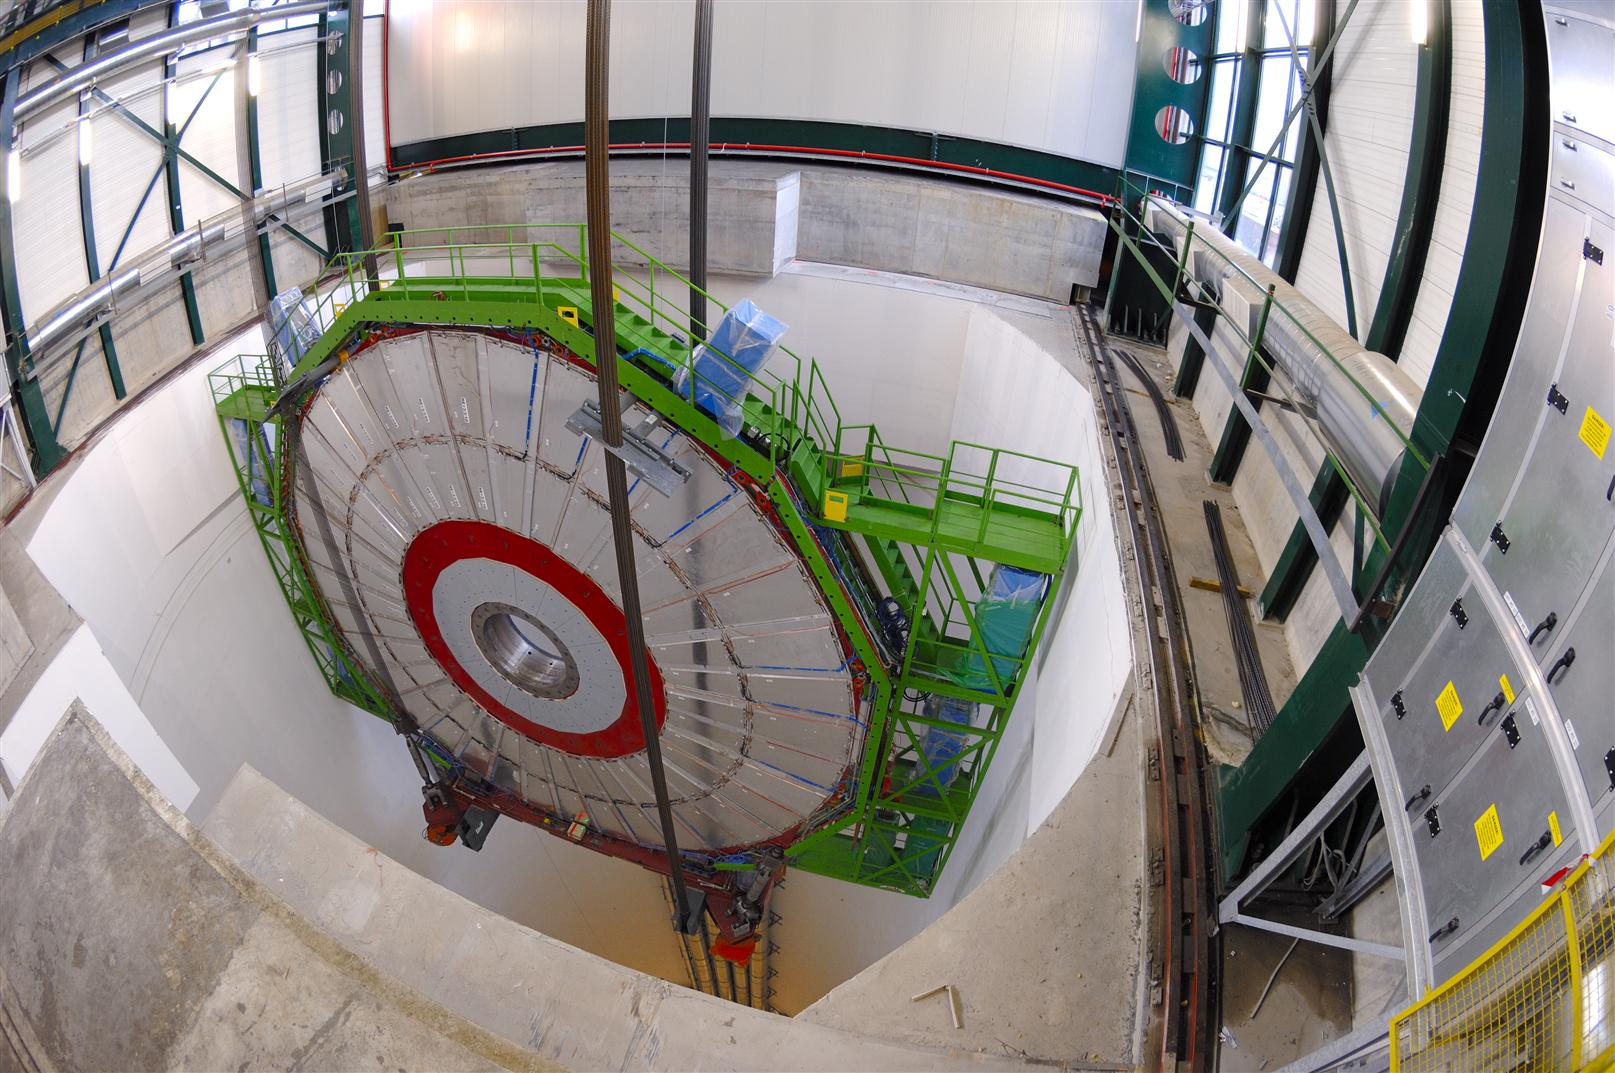
\includegraphics[width=\marginparwidth]{CMS/slice.jpg}
	\captionof{figure}{Descente d'une tranche de CMS.}
	\label{slice}
}
Chaque tranche à ensuite été descendue dans la caverne et assemblée à \SI{100}{\meter} sous terre (cf.Fig~\ref{slice}).
CMS est une détecteur cylindrique de \SI{24}{\meter} de long et de \SI{14.6}{\meter} de diamètre pour une masse de plus de \num{16000} tonnes (cf.Fig~\ref{cmsexploded}). Il est composé d'une succession de sous-détecteurs concentriques.

\begin{sidewaysfigure}
	\centering
	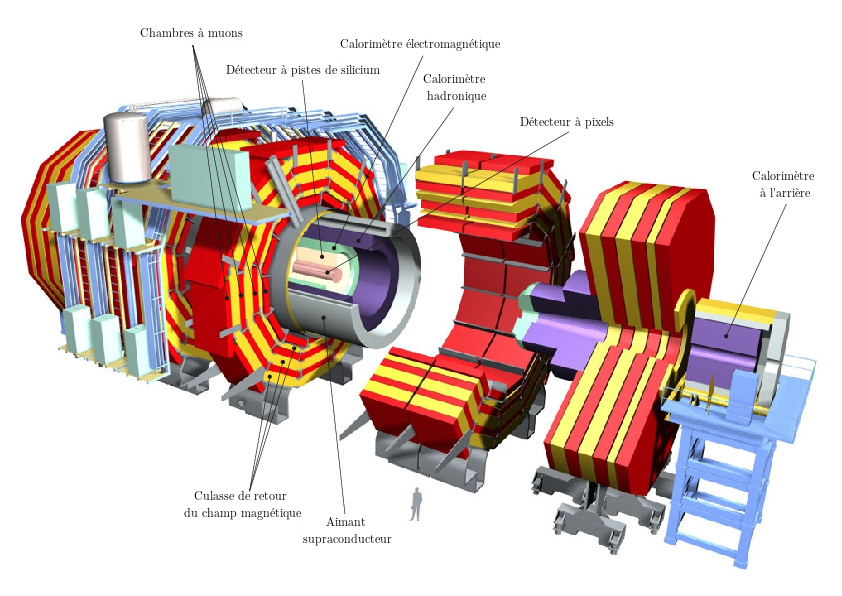
\includegraphics[width=0.80\textwidth]{CMS/cms.png}
	\caption{\label{cmsexploded}Vue éclatée du détecteur CMS.}
\end{sidewaysfigure}
\newpage
En partant du centre vers l'extérieur :
\begin{itemize}[label=$\bullet$]
	\item \textbf{Le trajectographe : } C'est le sous-détecteur le plus proche du point d'interaction. Il permet de reconstruire la trajectoires des particules chargées.
	 \item \textbf{Le calorimètre électromagnétique (ECAL\footnote{Pour \textit{Electromagnetic CALorimeter}.})}: Il permet de mesurer l'énergie des photons et des électrons.
	 \item \textbf{Le calorimètre hadronique (HCAL\footnote{Pour \textit{Hadronic CALorimeter}.})}: Il permet de mesurer l'énergie des hadrons.
	 \item \textbf{L'aimant supra-conducteur : } Il produit un champ de \SI{3.8}{\tesla} et permet de courber la trajectoire des particules chargées.
	 \item \textbf{Les chambres à muons : } Elles permettent d'identifier, reconstruire la trajectoire et mesurer l'énergie des muons. 
\end{itemize}
Chaque composant de CMS fera l'objet d'une description plus détaillée dans les paragraphes suivants.

\section{Les sous-détecteurs de CMS}
\subsection{Le trajectographe}
Le trajectographe de CMS (cf.Fig~\ref{trajectographe}) est le détecteur le plus proche du faisceau et du point de collision. Le trajectographe est composé de deux sous-détecteurs : le détecteur à pixels et le trajectographe à micro-pistes de silicium. Il a pour but de reconstruire les traces des particules chargées issues des collisions grâce à des suites d'impacts enregistrés par les couches du détecteur. La trace reconstruite permet de déterminer la charge et l'impulsion de la particule associée. En effet, une particule de charge $q$ qui se déplace dans un champ magnétique subit une force donné par la formule de \bsc{Lorentz}. La trajectoire de la particule dans le cas d'un champ magnétique d'intensité $B$ est hélicoïdale, de rayon $R_{c}$. Il est ainsi possible dans déduire l'impulsion transverse :
\begin{equation}
p_{T}=qBR_{c}
\end{equation}
En prenant les positions selon $r$ des hits, il est possible d'en déduire l'angle $\theta$, angle entre la trajectoire de la particule est le faisceau et donc de calculer l'impulsion totale:
\begin{equation}
p=\frac{p_{T}}{\sin\theta}
\end{equation}
\begin{figure}[ht!]
	\centering
	\includegraphics[width=0.65\textwidth]{CMS/tracker.png}
	\captionof{figure}{Schéma du trajectographe de CMS. Chaque trait représente un module du détecteur. Les lignes doubles correspondent à des modules mis dos à dos produisant des hits dit "stéréos". Le détecteur à pistes est composé de quatre sous-détecteurs : Les tonneaux internes (TIB), les tonneaux externes (TOB), les disques internes (TID) et les bouchons (TEC).}
	\label{trajectographe}
\end{figure}

\subsubsection{Le détecteur à pixels}
Le détecteur à pixels de CMS a récemment été remplacé afin de garder une trajectographie performante à des luminosités au dessus de \SI{2e34}{\per\square\centi\meter\per\second} et avec un empilement de plus de \num{50}. Ce remplacement a eu lieu du \num{28} février au \num{7} mars \num{2017} durant l'arrêt technique hivernal prolongé (EYETS). Le nouveau détecteur à pixels se compose d'un tonneau constitué de quatre couches de détection (BPIX) à des distances du faisceau $r=\SI{3.0}{\centi\meter}$, \SI{6.8}{\centi\meter}, \SI{10.2}{\centi\meter} et \SI{16}{\centi\meter} et d'une longueur de \SI{548.8}{\milli\meter} et de trois bouchons (FPIX) situé à $\pm$\SI{29.1}{\centi\meter}, $\pm$\SI{39.6}{\centi\meter} et $\pm$\SI{51.6}{\centi\meter} pour une couverture radiale allant de \num{4.5} à \SI{16.1}{\centi\meter}. Une comparaison entre l'ancien détecteur à pixel et le nouveau est donnée figure \ref{pixel}.

	\begin{figure}[ht!]
	\subfloat[Vue oblique-transverse comparant les couches des tonneaux de l'ancien (gauche) et du nouveau détecteur (droite).]{\includegraphics[width=.45\linewidth]{CMS/pixel.png}}
	\hfill
	\subfloat[Ancien détecteur à pixel (bas) et nouveau (haut).]{\includegraphics[width=.45\linewidth]{CMS/pixel2.png}}
	\caption{Comparaison entre le nouveau et l'ancien trajectographe à pixels.}
	\label{pixel}
\end{figure}

L'ajout d'une quatrième couche de détection dans le barrel assure une redondance lors de la reconnaissance de motifs et permet de réduire le taux d'erreurs lors d'empilement importants. Il assure également une sécurité au cas où la couche la plus proche du point d'interaction viendrait à se détériorer plus vite que prévu. Cependant, elle augmente le budget matière du détecteur, il a donc été nécessaire de repenser le support et les services afin d'être plus léger. Un nouveau système de refroidissement au \chemform{CO_2} ainsi que le déplacement des systèmes passifs (connectique, plaques d'électronique) hors du volume de trajectographie ont également été effectués (cf.Fig~\ref{pixel2}).

\begin{figure}[ht!]
	\centering
	\includegraphics[width=0.75\textwidth]{CMS/pixel3.png}
	\captionof{figure}{Vue explosée du nouveau détecteur à pixels. La figure montre les positions des différentes partitions FPIX et BPIX ainsi que leurs cylindres contenant leurs services respectifs. Les services nécessaires au détecteur (connectiques, fibres optiques, convertisseurs DC-DC sont situés à haut $\eta$, hors du volume de trajectographie).}
	\label{pixel2}
\end{figure}

Ce détecteur contient plus de \num{97} millions de pixels (\num{79} pour les BPIX et \num{18} pour les FPIX) mesurant \num{100}$\times$\SI{150}{\square\micro\meter} de section et \SI{250}{\micro\meter} d'épaisseur. Ces pixels sont regroupés en modules (\num{1184} pour BPIX et \num{672} pour FPIX) (cf.Fig~\ref{module}) de \num{66560} pixels  (\num{8}$\times$\num{2} ROCs) d'une épaisseur de \SI{75}{\micro\meter} pour la première couche du BPIX et \SI{250}{\micro\meter} pour le reste du BPIX et FPIX.

	\begin{figure}[ht!]
	\centering
	\subfloat[Module pour les couches \num{2} à \num{4} des BPIX et des FPIX (gauche) et de la couche \num{1} de BPIX (droite).]{\includegraphics[width=.46\linewidth]{CMS/module.png}}
	\hfill
	\subfloat[Schéma de l'électronique de lecture d'un module.]{\includegraphics[width=.46\linewidth]{CMS/module2.png}}
	\caption{Modules de pixels.}
	\label{module}
\end{figure}
\subsubsection{Le détecteur à pistes}
Le détecteur à pistes mesure \SI{5.5}{\meter} de long pour \SI{2.4}{\meter} de diamètre pour une aire active de \SI{198}{\square\meter} et est le plus grand détecteur au silicium jamais construit. Il comporte en tout \num{15148} modules pour un total de \num{9.3} millions de pistes lues par \num{76000} puces électroniques. Il peut être décomposé en quatre sous-détecteurs :

\begin{itemize}[label=$\bullet$]
\item \textbf{Le tonneau interne} (TIB) (cf.Fig~\ref{TIB}) pour  \textit{Tracker Inner Barrel} est composé de \num{2724} modules répartis en quatre couches. Chaque couche se compose de pistes de silicium d'une épaisseur de \SI{320}{\micro\meter} avec un pas de \SI{80}{\micro\meter} pour les deux premières couches et de \SI{120}{\micro\meter} pour les deux dernières. Elles sont orientées parallèlement au faisceau. Les deux premières couches sont composées de modules dits "stéréos" qui sont la juxtaposition de deux modules collés l'un l'autre avec un angle de \SI{100}{\milli\radian} entre les deux, ce qui permet d'avoir une résolution de \num{23} à \SI{34}{\micro\m} dans le plan transverse et de \SI{230}{\micro\meter} dans le plan longitudinal. Son rayon est compris entre \num{25} et \SI{52}{\centi\meter} et sa longueur couvre le domaine $|z|<$\SI{65}{\centi\meter}.

\item \textbf{Les disques internes} (TID) (cf.Fig~\ref{TID}) pour \textit{Tracker Inner Disk} sont composés de trois disques parallèles qui sont compris dans le domaine \SI{75}{\centi\meter}$<|z|<$\SI{110}{\centi\meter}. Chaque disque est composé de trois anneaux concentriques. Les \num{816} modules sont composés de strips d'une épaisseur de \SI{320}{\micro\meter} orientés radialement pour un pas compris entre \SI{81} et \SI{158}{\micro\meter}. Comme pour le TIB, les deux premiers modules sont "stéréos".
\marginpar
{
	\centering
	\includegraphics[width=\marginparwidth]{CMS/TOB_TEC.png}
	\captionof{figure}{Différents modules utilisés pour la construction du TOB et du TEC.}
	\label{TOB_TEC}
}
\item \textbf{Le tonneau externe } (TOB) (cf.Fig~\ref{TOB}) pour \textit{Tracker Outer Barrel} entoure les TIB et TID pour couvrir un espace entre \num{60} et \SI{100}{\centi\meter} en rayon et $|z|<$\SI{110}{\centi\meter}. Il est composé de \num{5208} modules (cf.Fig~\ref{TOB_TEC}) de pistes orientées parallèlement aux faisceaux et de pas compris entre \num{122} et \SI{183}{\micro\meter}. Ces modules sont répartis en six couches dont les deux dernières sont "stéréos". L'épaisseur de ces modules est de \SI{500}{\micro\meter}.   

\item \textbf{Les bouchons }(TEC) (cf.Fig~\ref{TEC}) pour \textit{Tracker End-Cap} sont composés de neuf disques chacun, de \num{4} à \num{7} anneaux concentriques. Ils couvrent \num{25}--\SI{110}{\centi\meter} en rayons et \num{120}--\SI{275}{\centi\meter} en $|z|$. Les deux premiers disques ainsi que le cinquième sont "stéréos". Les trois premiers anneaux sont composés de \num{1256} modules par bouchon (cf.Fig~\ref{TOB_TEC}) d'épaisseur \SI{320}{\micro\meter} et de pas inter-pistes compris entre \num{81} et \SI{158}{\micro\meter}. Les quatre anneaux suivant, sont composés de \num{1944} modules par bouchon (cf.Fig~\ref{TOB_TEC}), d'épaisseur \SI{500}{\micro\meter} de pas inter-strip \num{113}--\SI{172}{\micro\meter}.
\end{itemize}

	\begin{figure}[ht!]
	\centering
	\subfloat[Le TIB.]{\includegraphics[width=.40\linewidth]{CMS/TIB.jpg}\label{TIB}}
	\subfloat[Un TID.]{\includegraphics[width=.40\linewidth]{CMS/TID.jpg}\label{TID}}
	\\
	\subfloat[Le TOB.]{\includegraphics[width=.40\linewidth]{CMS/TOB.jpg}\label{TOB}}
	\subfloat[Un TEC.]{\includegraphics[width=.40\linewidth]{CMS/TEC.jpg}\label{TEC}}
	\caption{Photos des différents composants du détecteur à pistes.}
\end{figure}

\newpage
\subsection{Le calorimètre électromagnétique}
Le calorimètre électromagnétique de CMS ou \textit{Electromagnetic CALorimeter} (ECAL), permet de mesurer l'énergie et la direction des particules réagissant principalement à l'interaction électromagnétique. Ce sont surtout les photons et les électrons qui seront détectés; ils perdent leur énergie par des processus radiatifs. La distance caractéristique est donnée par la longueur de radiation $X_{0}$, dépendante du matériau, définie comme le libre parcours moyen pour le processus de radiation. Des photons de \SI{100}{\giga\eV} perdent à peu près toute leur énergie dans \num{20}$\times X_{0}$.
\begin{figure}[ht!]
	\centering
	\includegraphics[width=0.90\textwidth]{CMS/ECAL.png}
	\captionof{figure}{Schéma du ECAL de CMS.}
	\label{ECAL}
\end{figure}

Le calorimètre électromagnétique est composé de \num{75848} cristaux (cf.Fig~\ref{crystaux}) de \chemform{PbWO_4} (\SI{11}{\cubic\meter}, \num{92} tonnes) et peut se décomposer en trois sous-structures (cf.Fig~\ref{ECAL}) :
\begin{itemize}[label=$\bullet$]
	\item \textbf{Le tonneau} ou EB (cf.Fig~\ref{EB}) pour \textit{Electromagnetic Barrel} contient \num{61200} cristaux de tungstate de plomb. Le tonneau est divisé en \num{36} supermodules couvrant chacun la moitié de la longueur du tonneau. Chaque super-module contient \num{1700} cristaux de \num{22}$\times$\SI{22}{\square\milli\meter} et de longueur \SI{230}{\milli\meter}. Les cristaux sont arrangés de manière à former \num{170}-$\eta$ anneaux contenant \num{360} cristaux chacun. Un cristal couvre environ \SI{1}{\degree} en $\phi$. Le tonneau couvre une zone en pseudorapidité de $|\eta|<$\num{1.479}. Les photodiodes à avalanche (cf.Fig~\ref{APD}) (APD) sont utilisées pour détecter la scintillation.
	\marginpar
	{
		\centering
		\includegraphics[width=\marginparwidth]{CMS/Crystaux.png}
		\captionof{figure}{Un cristal de \chemform{PbWO_4}.}
		\label{crystaux}
	}
	
	\marginpar
	{
		\centering
		\includegraphics[width=\marginparwidth]{CMS/APD.png}
		\captionof{figure}{Un groupe de deux APD.}
		\label{APD}
	}
	\marginpar
	{
		\centering
		\includegraphics[width=\marginparwidth]{CMS/dee.jpg}
		\captionof{figure}{Un \textit{"Dee"}.}
		\label{DEE}
	}
	\marginpar
	{
		\centering
		\includegraphics[width=\marginparwidth]{CMS/20SCs.jpg}
		\captionof{figure}{Montage de \num{20} Super-Cristaux sur un des \textit{Dee}.}
		\label{SP}
	}
	\marginpar
	{
		\centering
		\includegraphics[width=\marginparwidth]{CMS/VPT.png}
		\captionof{figure}{Une VPT.}
		\label{VPT}
	}
	
	\item \textbf{Les bouchons} (EE) (cf.Fig~\ref{EE}) pour \textit{Electromagnetic End-cap} sont perpendiculaires aux faisceaux et ferment le EB. Ils sont situés à \SI{315}{\centi\meter} du point d'interaction et couvrent une section en $\eta$ allant de \num{1.479} à \num{3}. Chaque bouchon se décompose en deux demi-disques appelés \textit{"Dee"} (cf.Fig~\ref{DEE}). Chaque \textit{Dee} est constitué de \num{3662} cristaux de \num{2.86}$\times$\SI{2.86}{\centi\meter} et de longueur \SI{220}{\milli\meter} regroupés en matrices de \num{5}$\times$\num{5} qu'on appelle Super-Cristaux (cf.Fig~\ref{SP}). La scintillation est détectée par des phototriodes à vide (VPT) (cf.Fig~\ref{VPT}). Les cristaux de \chemform{PbWO_4} ont une grande densité ($\rho=$\SI{8.28}{\gram\per\cubic\centi\meter}), une longueur d'interaction $X_{0}$ assez courte de \SI{0.89}{\centi\meter} est un petit rayon de Molière ($r_{M}=$\SI{2.2}{\centi\meter}) ainsi qu'une grande vitesse de radiation (\num{80}\% dans \SI{25}{\nano\second}). 
	\item \textbf{L'initiateur de gerbe } (cf.Fig~\ref{PRESHOWER}), appelé \textit{Preshower} est placé entre le EB et le EE. Il consiste en deux couches de détecteurs de silicium de pas \SI{1.9}{\milli\meter} intercalées entre deux couches en plomb (\num{2}$X_{0}$ devant et \num{1}$X_{0}$ derrière la première couche de silicium). Il permet d'améliorer la précision de la mesure de la position de la gerbe électromagnétique et la discrimination $\gamma/\pi_{0}$. Il couvre une région comprise entre \num{1.653}$<|\eta|<$\num{2.6}.
\end{itemize}
\begin{figure}[ht!]
	\centering
	\subfloat[Le tonneau du ECAL (EB).]{\includegraphics[width=0.8\linewidth]{CMS/EB.jpg}\label{EB}}
	\\
	\subfloat[Un bouchon du ECAL (EE).]{\includegraphics[width=.40\linewidth]{CMS/EE.jpg}\label{EE}}
	\subfloat[Un des preshower du ECAL.]{\includegraphics[width=.40\linewidth]{CMS/preshower.jpg}\label{PRESHOWER}}
	\caption{Photos des différents composants du calorimètre électromagnétique.}
\end{figure}
\subsection{Le calorimètre hadronique}
	\marginpar
{
	\centering
	\includegraphics[width=\marginparwidth]{CMS/LAITON.jpg}
	\captionof{figure}{Photo de douilles de la marine russe réutilisées pour la construction du HCAL.}
	\label{LAITON}
}
	\marginpar
{
	\centering
	\includegraphics[width=\marginparwidth]{CMS/SCINTI.png}
	\captionof{figure}{Photo d'une tuile du HO avec des fibres WLS insérées dans les \num{4} $\sigma$-rainures.}
	\label{SCINTI}
}
\marginpar
{
	\centering
	\includegraphics[width=\marginparwidth]{CMS/MPPC.png}
	\captionof{figure}{Photo d'un MPPC.}
	\label{MPPC}
}
\marginpar
{
	\centering
	\includegraphics[width=\marginparwidth]{CMS/HPD.png}
	\captionof{figure}{Photo d'une HPD.}
	\label{HPD}
}
Le calorimètre hadronique de CMS ou \textit{Hadronic CALorimeter} (HCAL) (cf.Fig~\ref{HCAL}) permet de mesurer l'énergie et la direction des hadrons issus de l'hadronisation des quarks et gluons produits lors des collisions. Ce détecteur à une grande compacité spatiale et énergétique et est très compact car il se trouve pour une grande partie entre le ECAL et l'aimant supraconducteur. Cette disposition a nécessité de maximiser la quantité d'absorbeur et de minimiser les parties actives du détecteur. L'absorbeur est constitué de laiton (cf.Fig~\ref{LAITON}) qui possède une faible longueur d'interaction $\lambda_{l}$ et un faible taux de diffusions multiples. Les hadrons perdent majoritairement leur énergie par interaction nucléaire avec l'absorbeur. La plupart des hadrons sont stoppés avec \num{9}$\lambda_{l}$. Le laiton est également non magnétique ce qui est nécessaire vu l'emplacement du calorimètre. Le matériau actif est composé de feuilles de scintillateurs fluorescents (cf.Fig~\ref{SCINTI}). La scintillation est ensuite récoltée par des fibres optiques qui décalent la longueur d'onde de la lumière (WLS). Le signal est ensuite lu par des \textit{Multi-Pixel Photon Counter} (MPPC) (cf.Fig~\ref{MPPC}) pour le sous-détecteur \textit{Hadronic Outward calorimeter} et par des photodiodes hybrides (HPD) (cf.Fig~\ref{HPD}) pour les autres sous-détecteurs.
\begin{figure}[ht!]
	\centering
	\includegraphics[width=0.95\textwidth]{CMS/HCALSCHEME.png}
	\captionof{figure}{Schéma d'un quart d'une coupe du HCAL de CMS.}
	\label{HCAL}
\end{figure}

Le calorimètre hadronique couvre une zone en pseudo-rapidité jusqu'à $|\eta|<$\num{5.0}. Il possède plus de \num{70000} feuilles de scintillateurs. Il est composé de \num{4} sous-détecteurs subdivisés en tours : 
\begin{itemize}[label=$\bullet$]
	\item \textbf{Le tonneau} HB pour \textit{Hadronic Barrel calorimeter} (cf.Fig~\ref{HB}) couvre la région en pseudo rapidité $|\eta|<1.3$. Il est constitué de \num{36} quartiers couvrant \SI{20}{\degree} en $\phi$ découpés en quatre sous secteurs de \SI{5}{\degree} en $\phi$ et \num{16} sous secteurs en $\eta$. Un quartier possède \num{16} couches qui sont des empilements de scintillateurs de \SI{9}{\milli\meter} d'épaisseur pour les couches les plus externes et \SI{3.7}{\milli\meter} pour les autres et d'absorbeur de (\SI{40}{\milli\meter} de fer pour la première couche, \SI{50.5}{\milli\meter} de laiton pour les huit suivantes, \SI{56.5}{\milli\meter} de laiton pour les six suivantes et \SI{75}{\milli\meter} de fer pour la dernière). Les tours ont une segmentation de $\Delta\eta\times\Delta\phi=$\num{0.087}$\times$\num{0.087}.
	\item \textbf{Les deux bouchons} HE pour \textit{Hadronic End-cap calorimeter} (cf.Fig~\ref{HE}) couvrent les régions comprises entre $|\eta|>$\num{1.3} et $|\eta|<$\num{3.0}. Une zone inclinée à \SI{53}{\degree} par rapport à l'axe du faisceau et ne pointant pas vers le point d'interaction est laissée libre afin de permettre le passage des câbles et systèmes nécessaires au trajectographe et au calorimètre électromagnétique. Les bouchons sont segmentés en \num{18} quartiers de \SI{20}{\degree} en $\phi$ chacun composé de \num{14} tours en $\eta$. Les tours sont des empilements de scintillateurs de \SI{3.7}{\milli\meter} d'épaisseur et d'une couche d'absorbeur (\SI{9}{\milli\meter} pour la première couche et \SI{7.5}{\milli\meter} pour les suivantes). Une tour possède \num{19} couches de  scintillateurs en tout. Les \num{5} tours couvrant $|\eta|<$\num{1.74} ont une segmentation de $\Delta\eta\times\Delta\phi=$\num{0.087}$\times$\num{0.087} alors que les \num{8} couvrant \num{1.74}$<|\eta|<$\num{3.0} ont des segmentations allant de $\Delta\eta\times\Delta\phi=$\num{0.09}$\times$\num{0.174} à $\Delta\eta\times\Delta\phi=$\num{0.35}$\times$\num{0.174}.
	\item \textbf{Le calorimètre externe} HO pour \textit{Hadronic Outward calorimeter} (cf.Fig~\ref{HO}) est placé à l'extérieur de l'aimant supraconducteur. Il est constitué de couches de scintillateurs de \SI{10}{\milli\meter} d'épaisseur et couvre la région $|\eta|<$\num{1.26}. Ce sous-détecteur permet de récupérer l'énergie sortant du HB et assure une longueur d'interaction de plus de \num{10}$\lambda_{l}$. Le HO est composé de \num{5} anneaux de \SI{2.536}{\meter} de long selon $z$ numérotés $-$\num{2}, $-$\num{1}, \num{0}, $+$\num{1}, $+$\num{2} et de centre $z=-$\num{5.324}, \num{2.686}, \num{0}, \num{2.686} et \SI{5.324}{\meter} respectivement. Le premier anneau est composé de deux couches de scintillateurs de \SI{10}{\milli\meter} d'épaisseur placées en $r=$\SI{3.82}{\meter} et \SI{4.07}{\meter}. Les autres anneaux ne possèdent qu'une couche de scintillateur placé à $r=$\SI{4.07}{\meter}. Chaque anneau est segmenté en \num{12} secteurs en $\phi$. Chaque secteur est segmenté en \num{8}, \num{6} et \num{5} tuiles de scintillateurs (cf.Fig~\ref{SCINTI}) pour les anneaux \num{0}, $\pm$\num{1}, $\pm$\num{2} respectivement.
	\item \textbf{Les calorimètres très à l'avant} HF pour \textit{Hadronic Forward calorimeter} couvrent une zone en pseudo-rapidité comprise entre $|\eta|>$\num{3.0} et $|\eta|<$\num{5.0} et \SI{12.5}{\centi\meter}$<r<$\SI{130}{\centi\meter}. Ils sont situés à une distance $|z|=$\SI{11.2}{\meter} et font \SI{1.65}{\meter} de long. Ils consistent en un absorbeur de fer qui intègre des fibres de quarks résistantes aux radiations qui assurent la collection rapide de la lumière \bsc{Čerenkov}. La moitié de ces fibres font toute la longueur du détecteur (\SI{1.65}{\meter}) alors que d'autres commencent à \SI{22}{\centi\meter} (soit \SI{143}{\centi\meter} de long) du bord placées vers l'intérieur de CMS. Elles sont placées alternativement à une distance de \SI{5}{\milli\meter} l'une de l'autre en $r$  avec segmentation de $\Delta\eta\times\Delta\phi=$\num{0.175}$\times$\num{0.175}. Cette différence de longueur permet de séparer les cascades électromagnétiques des cascades hadroniques. La lumière est ensuite collectée par des tubes photo-multiplicateurs (PMT). Le HF est composé de \num{18} secteurs de \SI{20}{\degree} en $\phi$. Chaque secteur comporte \num{13} anneaux en $\eta$.
\end{itemize}
\begin{figure}[ht!]
\centering
\subfloat[Le tonneau du HCAL (HB).]{\includegraphics[width=.40\linewidth]{CMS/HB.jpg}\label{HB}}
\subfloat[Un bouchon du HCAL (HE).]{\includegraphics[width=.40\linewidth]{CMS/HE.jpg}\label{HE}}
\\
\subfloat[Installation du HO.]{\includegraphics[width=.40\linewidth]{CMS/HO.jpg}\label{HO}}
%http://cms.desy.de/e53612/e155171/e155181/
\subfloat[Un des HF du HCAL.]{\includegraphics[width=.40\linewidth]{CMS/HF.jpg}\label{HF}}
\caption{Photos des différents composants du calorimètre hadronique.}
\end{figure}
\vspace*{-0.3cm}	
\subsection{L'aimant supraconducteur}
\vspace*{-0.3cm}
L'aimant supraconducteur de CMS (cf.Fig~\ref{MAGNET}) est un solénoïde de \SI{5.9}{\meter} de diamètre pour \SI{12.9}{\meter} de longueur qui a été prévu pour créer un champ magnétique de \SI{4}{\tesla} à un courant de \SI{19.14}{\kilo\ampere}. À pleine puissance, il stocke une énergie de \SI{2.7}{\giga\joule}. Il est composé de \num{5} bobines en nobium-titane composées de \num{2168} spires, refroidies à une température de \SI{4.2}{\kelvin} par de l'hélium liquide. Une structure de retour de champ en fer de \num{11500} tonnes, composée de \num{5} culasses (cf.Fig~\ref{CULASSE}) et \num{2} bouchons, chacun composé de \num{3} disques, l'entoure et sert de structure de maintien des chambres à muons. L'épaisseur totale du retour est d'environ \SI{1.5}{\meter} (l'épaisseur du troisième disque des bouchons et du premier anneau du tonneau est de \SI{30}{\centi\meter}) et les autres disques des bouchons ainsi que les deuxième et troisième anneaux du tonneau font \SI{60}{\centi\meter}. L'épaisseur à été étudiée afin d'être suffisante pour absorber les hadrons qui traverseraient les calorimètres et l'aimant tout en restant assez fin pour éviter les pertes radiatives pour les muons.
\marginpar
{
	\centering
	\includegraphics[width=\marginparwidth]{CMS/CULASSE.jpg}
	\captionof{figure}{Photo d'une culasse.}
	\label{CULASSE}
}
\begin{figure}[ht!]
	\centering
	\includegraphics[width=0.50\textwidth]{CMS/MAGNET.png}
	\captionof{figure}{Schéma de l'aimant supra-conducteur de CMS.}
	\label{MAGNET}
\end{figure}
\newpage
La figure \ref{CHAMP} montre une simulation par éléments-finis de la valeur du champ magnétique en fonction de la position.
\begin{figure}[ht!]
	\centering
	\includegraphics[width=0.90\textwidth]{CMS/CHAMP.png}
	\captionof{figure}{Valeur du champ magnétique (gauche) et lignes de champ (droite) selon une coupe longitudinale du détecteur CMS, prédits par la simulation. Pour une valeur du champ central de \SI{3.8}{\tesla}.}
	\label{CHAMP}
\end{figure}
\subsection{Le spectrographe à muons}
\label{RPCPRE}
Le spectographe à muons (cf.Fig~\ref{CMS1}, Fig.~\ref{CMS2}) a pour but d'identifier les muons, de mesurer avec précision leur quantité de mouvement et de déclencher sur les événements contenant des muons.
\marginpar
{
	\centering
	\includegraphics[width=\marginparwidth]{CMS/MUON.png}
	\captionof{figure}{Quart d'une coupe dans le plan transverse du détecteur CMS montrant la trajectoire d'un muon (courbe bleue).}
	\label{MUON}
} Les muons ont un très grand pouvoir de pénétration. Il est donc possible d'utiliser à la fois les traces chargées laissées dans le trajectographe et dans des détecteurs placés après l'aimant pour les identifier et les reconstruire de manière précise. Une bonne résolution de la quantité de mouvement des muons et leur bonne identification est obtenue grâce au champ magnétique intense de l'aimant et du retour de champ dans la culasse qui assure une trajectoire avec une double courbure. Cette culasse doit contenir des détecteurs de grande taille afin d'augmenter la probabilité de détection. Ils faut donc qu'ils soient peu onéreux et fiables. Il faut également que ces détecteurs ne soient pas atteints par d'autres particules afin d'assurer un signal propre, pour ce faire la distance depuis l'aimant jusqu'à la dernière station du spectrographe et de l'ordre de \num{16} longueurs de radiation, ce qui évite le bruit de fond hadronique résiduel venant du faisceau.

\begin{sidewaysfigure}
\centering
\includegraphics[width=0.80\textwidth]{CMS/CMSLONG.png}
\captionof{figure}{Coupe longitudinale d'un quart de CMS.}
\label{CMS1}
\end{sidewaysfigure}


\begin{figure}[p]
\centering
\includegraphics[width=0.98\textwidth]{CMS/CMSTRANS.png}
\captionof{figure}{Coupe transversale de la partie centrale CMS.}
\label{CMS2}
\end{figure}

Le spectrographe à muons, est composé de \num{3} sous-détecteurs :
\begin{itemize}[label=$\bullet$]
	\item \textbf{Les chambres à dérive} DT pour \textit{Drift Tube} (cf.Fig~\ref{DT}) sont présentes seulement dans le tonneau où le flux de muons est faible tout comme le bruit de fond des neutrons. Le champ magnétique est également assez faible ($\sim$\SI{0.4}{\tesla}) et uniforme. Ce détecteur est constitué de \num{250} chambres insérées dans la culasse de CMS. Elles sont disposées en quatre couches selon $r$ à des distances $r=$\num{4.0}, \num{4.9}, \num{5.9} et \SI{7.0}{\meter}. La culasse est composée selon l'axe $z$ de \num{5} roues numérotées de $-$\num{2} à \num{2}, chacune comportant \num{12} (sauf pour MB4 qui en possède \num{14} (cf.Fig~\ref{CMS2})) secteurs dans le plan transverse numérotés à partir de $\phi=$\num{0} et couvrant \SI{30}{\degree}. Ce détecteur couvre une zone en pseudo rapidité $|\eta|<$\num{1.2}. Chaque chambre est constituée de \num{8} couches de tubes (cf.Fig~\ref{DT1}) mesurant la courbure de la trajectoire des muons selon $\phi$ et \num{4} couches pour la courbure selon $\eta$. Chaque ensemble de \num{4} couches est appelé super-couche (\textit{superlayer}). Les deux super-couches mesurant $\phi$ sont séparées par \SI{20}{\centi\meter} d'aluminium en nid d'abeilles. Seules les chambres de MB4 ne possèdent pas de \textit{superlayer} mesurant $\eta$ bien que la distance entre les deux \textit{superlayers} reste la même.
	\begin{figure}[ht!]
		\centering
		\includegraphics[width=0.40\textwidth]{CMS/DTchamber.png}
		\captionof{figure}{Schéma d'une chambre à dérive.}
		\label{DT1}
	\end{figure}

    Les tubes d'une couche de la chambre sont constitués de \num{5} électrodes : un fil d'acier inoxydable au centre du tube composant l'anode, \num{2} pistes servant de cathodes et \num{2} pistes servant d'électrodes et à mettre en forme le champ électrique. Ces deux électrodes améliorent l'uniformité du champ à l'intérieur du tube loin du fil et améliorent ainsi la résolution spatiale. Le tube est rempli d'un gaz de \chemform{ArCO_2} \num{85}/\num{15}. Lorsqu'une particule traverse le tube, elle ionise le gaz qui libère des électrons qui sont ensuite accélérés vers l'anode. Une avalanche se crée près du fil, où le champ électrique est intense, ce qui induit un signal sur le fil. Le temps de dérive est d'environs \SI{380}{\nano\second}. 
    
    	\begin{figure}[ht!]
    	\centering
    	\includegraphics[width=0.45\textwidth]{CMS/DTTUBE.png}
    	\captionof{figure}{Schéma d'un tube d'une chambre à dérive.}
    	\label{DT2}
    	\end{figure}
    En estimant le temps d'arrivée des électrons sur l'anode, en supposant le temps d'interaction connu et en ayant trois couches d'un superlayer touchées, il est possible d'estimer la position et le temps de la trace. Dans un superlayer une résolution de \SI{20}{\milli\radian} en angle, de \SI{100}{\micro\meter} en position et de quelques \si{\nano\second} en temps est atteinte.
    
    \item \textbf{Les chambres à pistes cathodiques} CSC pour \textit{Cathode Strip Chambers} (cf.Fig~\ref{CSC}) sont présentes dans les bouchons où le flux de muons ainsi que le bruit de fond sont importants, le champ magnétique est également non-uniforme. Ces chambres ont un temps de réponse très court, une granularité fine et sont presque insensibles à la non-uniformité du champ magnétique. Ce détecteur couvre les zones de pseudo-rapidité \num{0.9}$<=|\eta|<=$\num{2.4} et consiste en \num{468} chambres installées dans les bouchons. Chaque bouchon comprend \num{4} stations nommées ME1, ME2, ME3 et ME4. Chaque station comprend \num{2} anneaux (sauf ME1 qui en comprend \num{3}) segmentés en \num{36} chambres couvrant chacune un angle de \SI{10}{\degree} en $\phi$.
    
    Les chambres (cf.Fig~\ref{CSC2}) sont constituées de \num{6} couches contenant un mélange de gaz (\num{40}\% \chemform{Ar} \num{50}\% \chemform{CO_2} qui assure un bon gain et \num{10}\% \chemform{CF_4} afin d'empêcher la polymérisation près des fils.) ainsi qu'un plan de pistes de cathodes radiales et de fils séparés de \SI{3}{\milli\meter} constituant les anodes placées orthogonalement aux pistes (sauf pour les premier anneaux de ME1 ou les fils sont orientés à \SI{26}{\degree} afin de compenser la force de \bsc{Lorentz} due au champ magnétique de \SI{4}{\tesla} dans cette zone). Le nombre total de pistes est de \num{220 000} pour plus de \num {2 000 000} fils.
    
    Lorsqu'une particule chargée traverse une CSC, elle ionise le gaz. Les électrons sont accélérés vers le fils d'anode. Le mouvement de ces charges induit un signal sur les pistes cathodes et les fils anodes de la chambre. Le temps de dérive est beaucoup plus rapide que pour les DT mais la résolution spatiale est plus faible : \SI{150}{\micro\meter} dans le plan transverse.
    \begin{figure}[ht!]
    	\centering
    	\includegraphics[width=0.60\textwidth]{CMS/CSC2.png}
    	\captionof{figure}{Schéma d'une chambre CSC.}
    	\label{CSC2}
    \end{figure}
    
	\item \textbf{Les chambres à plaques résistives} ou \textit{Resistive Plate Chambers} (RPC) (cf.Fig~\ref{RPC}) forment un système très efficace pour déclencher sur les muons même à bas $p_{T}$ et sur une zone en pseudo rapidité très large ($|\eta|<$\num{1.6}) grâce à son excellente résolution temporelle ($\sim$\si{\nano\second}). Elles complètent les détecteurs CSC et DT dont les résolutions spatiales sont beaucoup plus élevées. Les RPC permettent d'assigner avec une plus grande précision le bon temps de croisement de faisceau pour les muons. Elles sont présentes à la fois dans le tonneau et les bouchons. Dans le tonneau \num{480} sont réparties en \num{6} couches, \num{2} pour MB1 et MB2 et \num{1} pour MB3 et MB4. La redondance en MB1 et MB2 permet de déclencher sur les muons de bas $p_{T}$ qui pourraient être arrêtés avant d'atteindre MB3. Pour les bouchons, les \num{432} chambres sont répartis en trois disques noté RE1, RE2 et RE3 pour chaque bouchon. Chaque disque est composé de \num{3} anneaux RE*/1 RE*/2 RE*/3 avec * représentant le numéro du disque. Seuls les anneaux \num{2} et \num{3} sont instrumentés. Chaque anneaux est segmenté en \num{36} chambres couvrant $\phi=$\SI{10}{\degree}.
	
	Les RPC sont des chambres à double \textit{gaps} (cf.Fig~\ref{RPC2}) qui opèrent en mode avalanche afin de fonctionner même à haut flux de particules $\sim$\SI{100}{\hertz\per\square\centi\meter}. Un gap est constitué de deux plaques de bakélite qui servent d'électrodes entres lesquelles circule un gaz. Des pistes de lecture sont insérées entre les deux gaps. Le système des RPC dans CMS ainsi que le fonctionnement d'une RPC sont expliqués dans le prochain chapitre.
	
	  \begin{figure}[ht!]
		\centering
		\includegraphics[width=0.80\textwidth]{CMS/RPC2.jpg}
		\captionof{figure}{Schéma en vue éclatée d'un gap d'une RPC et des pistes de lecture.}
		\label{RPC2}
	\end{figure}
	
	
\end{itemize}
    \begin{figure}[ht!]
	\centering
	\subfloat[Une cassette contenant une chambre DT et RPC.]{\includegraphics[width=0.40\linewidth]{CMS/DT.jpg}\label{DT}}
	\subfloat[Une chambre CSC.]{\includegraphics[width=.40\linewidth]{CMS/CSC.jpg}\label{CSC}}
	\\
	\subfloat[Une chambre RPC.]{\includegraphics[width=.40\linewidth]{CMS/RPC.jpg}\label{RPC}}
	\caption{Photos des différents composants du spectrographe à muons.}
\end{figure}

\section{Le système de déclenchement et d'acquisition de données}
Chaque type de particules lors de son passage dans CMS va créer des types de traces particulières qui vont être enregistrées sous forme électronique par les sous-détecteurs le composant. La figure \ref{particules} montre une vue schématique des traces laissées par différents types de particules dans les sous-détecteurs de CMS.

	  \begin{figure}[ht!]
	\centering
	\includegraphics[width=0.52\textwidth]{CMS/particles.png}
	\captionof{figure}{Schéma des traces laissées par différents types de particules dans les sous détecteurs de CMS.}
	\label{particules}
\end{figure}

Les faisceaux ont une fréquence de croisement de \SI{40}{\mega\hertz}, chaque événement créé lors de ces collisions génère environ un Méga-octets de données. Le flux de données est bien trop important pour être stocké ($\sim$\SI{40}{\tera\byte\per\second}). Celui-ci doit donc être réduit, il est donc nécessaire de rejeter des événements afin d'obtenir une fréquence d'acquisition de l'ordre de \SI{300}{\hertz} tout en continuant d'enregistrer les événements intéressants pour la physique. Cette étape est réalisée par le système de déclenchement ou \textit{trigger}. La réduction d'un facteur \num{e5} du taux d'acquisition des données est impossible à réaliser en une seule fois, le \textit{trigger} est donc constitué de deux étapes appelées \textit{Level-1 Trigger} (L1) qui réduit le flux d'événements à \SI{100}{\kilo\hertz} et \textit{High-Level Trigger} (HLT) qui réduit ensuite ce flux à \SI{300}{\hertz}.

\subsection{Le déclenchement de niveau I (L1)}
Le trigger de niveau I (L1) (cf.Fig~ \ref{L1}) opère à la fréquence de collision des faisceaux (\SI{40}{\mega\hertz}). L'électronique des détecteurs lit et stocke les  signaux électriques dans une mémoire tampon de \num{128} événements de collisions soit \SI{3.2}{\micro\second}. Le système de déclenchement possède donc \SI{3.2}{\micro\second} pour  décider s'il doit envoyer les données au déclenchement de haut niveau HLT. Chaque \SI{25}{\nano\second}, un nouvel événement rentre dans la mémoire tampon et la décision de garder ou non l'événement arrivé \SI{3.2}{\micro\second} plus tôt est prise. Les \SI{3.2}{\micro\second} correspondent à l'envoi des données depuis l'électronique des calorimètres et du spectrographe à muons vers la caverne de services qui contient les processeurs gérant la prise de décision, le retour d'un signal pour le rejet ou l'acceptation de l'événement, le délai de synchronisation entre les parties du détecteur ainsi que le temps de prise de décision en lui-même ($\sim$\SI{1}{\micro\second}). 

	  \begin{figure}[ht!]
	\centering
	\includegraphics[width=0.70\textwidth]{CMS/L1.png}
	\captionof{figure}{Schéma du Level-1 Trigger (L1).}
	\label{L1}
\end{figure}

Chacun des trois sous-détecteurs du spectrographe à muons utilise son propre système de déclenchement. Les DT et CSC créent des segments de traces. Ces segments ne sont conservés que s'il pointent vers le point d'interaction. Deux (trois) traces par DT (CSC) sont envoyées au \textit{Drift Tube Track Finder} (DTTF) (\textit{Cathode Strip Chamber Track Finder }(CSCTF)) qui cherchent des correspondances entre les traces et assignent un niveau de qualité aux valeurs $\eta$, $\phi$, à la charge et à la quantité de mouvement trouvées par ces correspondances. Quatre candidats muons sont envoyés au \textit{Global Muon Trigger} (GMT) par les \textit{"Finder"}. Pour les RPC, la sélection est basée sur une coïncidence spatiale et temporelle entre les différentes couches. Le \textit{Pattern Comparator} compare les signaux venant des \num{4} stations à des patrons prédéfinis afin de trouver les candidats muons et \num{8} d'entre eux (\num{4} pour les bouchons \num{4} pour le tonneau) sont envoyés au GMT. Le GMT reçoit tous ces candidats et combine ceux trouvés dans plusieurs sous-detecteurs. Il assigne ensuite un niveau de qualité à ces nouveaux candidats et envoie les \num{4} meilleurs d'entre eux au \textit{Global Trigger} (GT).

Les calorimètres sont réunis en tours de déclenchement qui correspondent aux super-cristaux pour le ECAL. Un candidat est trouvé pour chaque tour du ECAL et HCAL. Le \textit{Trigger Primitive Generator} est responsable de sommer les énergies venant des différents composants des tours.  Le \textit{Regional Calorimeter Trigger} (RCT) reçoit les candidats du ECAL et HCAL qui sont répartis en \num{18} \textit{crates} qui couvrent la moitié des détecteurs en $z$ et \SI{40}{\degree} en $\phi$ et fournissent au \textit{Global Calorimeter Trigger} chacun \num{4} candidats $e/\gamma$ isolés et \num{4} candidats non-isolés. Le GCT fournit des informations sur l'isolation et la compatibilité avec des particules d'ionisation minimale au système \textit{trigger} des muons et classe les candidats $e/\gamma$ par niveau de qualité et envoie les \num{4} meilleurs isolés et les \num{4} meilleurs non-isolés au GT. Le GT possède également des informations sur les jets, l'énergie transverse totale, etc.

La décision finale est faite par le \textit{Global Trigger} à partir de conditions programmables demandant la présence d'objets ou d'énergie en quantité ou valeurs prédéfinies. Ces conditions forment un chemin de déclenchement. Le \textit{Global Trigger} permet de programmer et de tester jusqu'à \num{128} chemins en parallèle. 

\subsection{Le déclenchement de haut niveau (HLT)}
Si l'événement est sélectionné par le L1, il est envoyé au déclenchement de haut niveau (HLT) et les données sont transmises à une ferme de calcul de plusieurs milliers d'ordinateurs  dont chaque processeur exécute le même code de déclenchement (\textit{HLT Menu}) séquentiellement afin de réduire le temps nécessaire à l'élimination d'un événement et d'améliorer le temps de décision qui doit être de l'ordre de \SI{100}{\milli\second} par événement. Il permet de passer à un flux de donnée de \SI{300}{\hertz}. Durant cette phase, les données du \textit{tracker} sont utilisées contrairement au L1.

\section{Mises à niveau et amélioration de CMS}
Le détecteur CMS à déjà subi de nombreuses améliorations depuis le début de sa mise en service (SiPM dans le HO, nouveau trajectographe à pixels\ldots). Cependant, la mise à niveau du LHC vers le HL-LHC prévoit de multiplier la luminosité par \num{7.5}, ce qui représente un défi pour CMS qui doit se mettre à niveau pendant les arrêts LS2 et LS3 afin de pouvoir s'adapter à cette luminosité et au \textit{pile-up} supplémentaire que cela va engendrer ($\sim$\num{140}--\num{200} événements de \textit{pile-up}). Parmi les mises à niveaux programmées citons \cite{Collaboration:1355706} \cite{Contardo:2020886} :
\begin{itemize}[label=$\bullet$]
	\item Le remplacement des HPD dans les sous-détecteurs HB, HE du calorimètre hadronique pendant le LS2 par des SiPM (comme actuellement dans le HO).
	\item Le remplacement complet du trajectographe durant LS3 (cf.Fig~\ref{tracker2}). La granularité doit être multipliée par \num{4} afin de garder une bonne performance de reconstruction malgré l'augmentation du \textit{pile-up}. Pour cela, les pistes du trajectographe à pistes seront raccourcies et le détecteur sera également plus léger afin d'obtenir une meilleure résolution en $p_{T}$ et une conversion des $\gamma$ plus faible. Le trajectographe à pixels aura des pixels et des senseurs plus petits afin d'améliorer la résolution du paramètre d'impact et une meilleure séparation des traces. Plus de \num{10} disques additionnels dans chaque bouchon seront installés afin de couvrir une zone en rapidité jusqu'à $|\eta|=$\num{4}.
	\begin{figure}[ht!]
		\centering
		\includegraphics[width=0.88\textwidth]{CMS/tracker2.png}
		\captionof{figure}{Schéma d'un quart du trajectographe prévu pour la mise à niveau de CMS.}
		\label{tracker2}
	\end{figure}
	\item Les bouchons des calorimètres devront être remplacés par des calorimètres de haute granularité \textit{High Granularity Calorimeter} (HGC) d'une profondeur totale de $\sim$\num{10}$\lambda_{I}$ qui fourniront des images tridimensionnelles détaillées des gerbes. La section électromagnétique est composée d'une trentaine de couches de tungstène et de plaques de cuivre intercalées avec des capteurs de silicium comme matière active. Les capteurs auront des aires variables inférieures à $\sim$\SI{1,0}{\square\centi\meter}. La section électromagnétique fait environs \num{25}$X_0$ et une longueur d'interaction ($\lambda_{I}$). La partie hadronique possède \num{12} plaques de laiton et de cuivre intercalées avec des capteurs de silicium d'une longueur représentant \num{3,5}$\lambda_{I}$ ce qui couvre la majorité d'une gerbe hadronique. Il est suivi d'un "calorimètre hadronique à l'arrière" de conception similaire à l'actuel HE (des plaques en laiton intercalées avec des carreaux scintillants en plastique lus avec des fibres optiques à décalage de longueur d'ondes). La conception de ce calorimètre à grande granularité s'appuie sur les concepts du ILC/CALICE pour la mesure 3D des gerbes.
	\item le temps de latence du L1 sera augmenté jusqu'à \SI{12.5}{\micro\second} ce qui permettra au système de reconstruction et d'identification des traces d'utiliser à la fois celles venant des calorimètres et celles du spectrographe à muons. Pour cela l'électronique de certains sous-détecteurs déjà existant devra être mise à niveau. La fréquence des données en sortie est estimée à \SI{5000}{\hertz} (\SI{7000}{\hertz}) avec \num{140} (\num{200}) événements de \textit{pile-up}. Le trigger L1 aura également les informations des traces fournies par le trajectographe pour des traces avec $p_{T}\geq$\SI{2}{\giga\eV}. Cela permettra un meilleur pouvoir de rejet du bruit de fond dès le début de la sélection des événements. Un tout nouveau L1 pour les calorimètres et le spectrographe à muons sera également mis en service (cf.Fig~\ref{L1_2}).
	\begin{figure}[ht!]
		\centering
		\includegraphics[width=0.55\textwidth]{CMS/L1_2.png}
		\captionof{figure}{Schéma du nouveau L1 pour la partie calorimètre et muons.}
		\label{L1_2}
	\end{figure}
\item Le trajectographe à muons dans les bouchons ne possède actuellement que des CSC dans la zone \num{1.6}$<|\eta|<$\num{2.4}. C'est la seule région du trajectographe qui ne possède pas de RPC afin d'assurer une redondance malgré le fait qu'il s'agisse d'une région dont la résolution de la quantité de mouvement est moins bonne et dont le bruit de fond est important. Afin d'améliorer le L1 dans cette région il est proposé d'instrumenter cette zone avec des chambres de nouvelle technologie. Il est donc prévu d'utiliser des \textit{Gas Electron Multiplier} (GEM) dans les stations ME1 et ME2 qui présentent une bonne résolution spatiale et qui résistent au champ magnétique important présent dans ces zones. Elles permettront d'améliorer la résolution en quantité de mouvement et d'améliorer la correspondance avec les traces dans le \textit{Global Muon Trigger}. Pour les deux dernières zones ME3 et ME4, des RPC de meilleure granularité et de bonne résolution temporelle seront utilisés afin de réduire le bruit de fond.  De plus, une nouvelle station ME0 de GEM sera insérée dans l'espace libéré par les nouveaux bouchons de CMS, ce qui augmentera la couverture de détection des muons jusqu'à $|\eta|\approx$\num{3} (cf.Fig~\ref{end}). 
	\begin{figure}[ht!]
	\centering
	\includegraphics[width=0.60\textwidth]{CMS/endcap.png}
	\captionof{figure}{Schéma d'un quart du détecteur CMS montrant les différentes technologies qui seront utilisées dans les bouchons du spectrographe à muons.}
	\label{end}
\end{figure}
\end{itemize}
Ce dernier point et plus particulièrement la caractérisation de détecteurs à plaques résistives de verres de basse résistivité est l'objet de cette thèse et sera développé dans les chapitres suivants. 
\chapter{Les Chambres à plaques résistives de CMS}
\renewcommand\chapterillustration{RPC/rpc}
\ThisULCornerWallPaper{1}{\chapterillustration}
\minitoc

\lettrine[lines=4, slope=-0.5em]{D}{ans} ce chapitre,une description générale des chambres à plaques résistive (RPC) ainsi qu'une description détaillée des chambres RPC utilisées dans CMS et de leurs électroniques. Une description des mises à niveaux se rapportant à ces détecteurs, notamment dans les bouchons sera également présentée.

\section{Les chambres à plaques résistives (RPC)}

 \marginpar
{
	\centering
	\includegraphics[width=\marginparwidth]{RPC/Geiger.png}
	\captionof{figure}{Photo d'un des premiers tubes Geiger-Müller fabriqué en 1932 par Hans Geiger pour une utilisation en laboratoire.}
	\label{Geiger}
}
Les RPC pour \textit{Resistive Plate Chambers} font partie d'une famille de détecteurs appelé détecteurs gazeux. Ces détecteurs ont joué un rôle dès le début de la Physique des Hautes Énergies dans la détection de nouvelles particules. Depuis le premier détecteur gazeux, le compteur proportionnel à un seul fil \textit{Single-wire proportional counter} inventé par Rutherford et Geiger, puis le compteur Geiger-Müller (cf.fig\ref{Geiger}) présenté en 1928, les détecteurs gazeux n'ont cessé de se perfectionner et devenir plus rapide, efficaces et permettent de couvrir de grandes surfaces de détections à des coûts très modestes.

\subsection{Les détecteurs gazeux}
Les détecteurs gazeux reposent tous sur le même principe simple. Lorsqu'une particule traverse un gaz, elle l'ionise. Les ions et électrons créés lors de cette ionisation peuvent être accélérés grâce à une champ électrique. En choisissant judicieusement l'intensité du champ électrique, c'est à dire en appliquant une tension aux bornes des électrodes, les électrons peuvent gagner assez d'énergie pour ioniser le gaz à leur tour (seconde ionisation) et commencer une multiplication de charge. Le nombre de charges libérées détermine le mode de fonctionnement du détecteur. Le gaz est également un élément important du détecteur et a un rôle important sur le mode de fonctionnement de celui-ci. Le déplacement des ces charges à l'intérieur du gaz induit un déplacement de charges sur les électrodes, et crée un signal qui peut être récupéré par une électronique et donner une information sur le temps et la position de la trajectoire de la particule incidente. Ces charges peuvent donner lieu à un mode dit "streamer" voire donner lieu à la création d'étincelles entre l'anode et la cathode. La figure \ref{mult} montre le facteur d'amplification, ou le gain du gaz en fonction du voltage appliqué. 

\begin{figure}[h!]
	\centering
	\includegraphics[width=0.95\textwidth]{RPC/gasgain.png}
	\captionof{figure}{Évolution typique de gain du gaz en fonction du voltage appliqué (en échelle arbitraire).}
	\label{mult}
\end{figure}

Six régions peuvent être définies :

\begin{itemize}
	\item \textbf{I} Les paires d'électrons-ions primaires se recombinent avant d'avoir le temps de produire une seconde ionisation.
	\item \textbf{II} Les charges dues à l'ionisation primaire sont entièrement récoltées sur les électrodes. Le facteur d'amplification reste constant même si le voltage est augmenté.
	\item \textbf{III} Les charges produites par l'avalanche sont proportionnelles aux charges produites lors de la première ionisation. Les charges collectées augmentent fortement avec la tension appliquée.
	\item \textbf{IV} Cette région est la limite de proportionnalité, l'avalanche se transforme en streamer, un plasma d'ions et d'électrons.
	\item \textbf{V} Les streamers connectent les électrodes et produisent des étincelles visible. Les compteurs Geiger-Müller et les chambres à étincelles fonctionnent dans ce mode.
	\item \textbf{VI} Des décharges électrique se produisent même sans le passage de particules pour ioniser le gaz. Ce mode peut détruire le détecteur.
\end{itemize}

Les détecteurs gazeux à fils ont une résolution temporelle de l'ordre de la centaine de nanoseconde. Cela est dû au champ électrique en $\frac{1}{r}$, qui fait que la zone d'amplification se situe proche du fil et les électrons doivent atteindre cette zone avant d'être amplifiés et de démarrer l'avalanche.

En utilisant un champ électrique uniforme et important, une meilleure résolution temporelle est atteignable.

Le premier détecteur gazeux utilisant cette méthode est le compteur à étincelle "Spark Counter" développé dans les années 1948 , un détecteur qui présente une géométrie plane. Il est généralement constitué de deux électrodes métalliques entre lesquelles est présent un gaz. Le passage d'une particule ionise ce gaz et crée une avalanche qui rentre à un certain moment en mode streamer. Un plasma se crée entre les deux électrodes, les électrodes se déchargent et amènent à la création d'une étincelle. Ce type de détecteur présente un signal qui ne nécessite pas d'amplification, cependant le temps nécessaire à le recharge des electrodes est de l'ordre de quelques millisecondes. De plus la surface du détecteur ne doit pas être trop grande (~cm2) afin de ne pas détruire les électrodes lors des décharges.

Afin de résoudre ces problèmes, les électrodes métalliques peuvent être remplacées par des plaques de matériaux de haute résistivité ($10^{9}$ à $10^{10}$ohms). Ceci permet de limiter l'aire de décharge des électrodes autour du signal ainsi qu'une mélange de gaz absorbant les photons afin d'éviter le mode streamer. Ce qui permet le fonctionnement du détecteur à des flux de particules plus important. Le champs électrique baissant localement du fait de la recharge plus lente des électrodes le développement d'avalanches successives au même endroit est limité tout en laissant le détecteur opérationnel hors de cette zone.

\subsubsection{Naissance des RPC}
En 1981 R.Santonico et R.Cardarelli développent les Resistive Plate Chamber (RPC). Ce détecteur utilise un matériau peu coûteux est très utilisé de haute résistivité (~$10^{10}$ohms), le High Pressure Laminate (HPL) fait de melamine ou résines phénol-formaldéhyde (Bakélite). Le temps de décharge d'une électrode d'une telle résistivité recevant une charge $Q_{0}$ est donné par :
\begin{equation}
Q(t)=Q_{0}e^{\frac{-t}{\rho\epsilon_{0}\epsilon_{r}}}=Q_{0}e^{\frac{-t}{\tau}}
\end{equation}
avec $\rho$ la resistivité volumique du matériau, $\epsilon_{0}$ la permittivité du vide et $\epsilon_{r}$ la permitivité relative du matériau.
Les charges présentes sur les électrodes réduisent la haute tension appliquée et donc le champ électrique à l'endroit des charges. Le détecteur devient inefficace pour cette periode de temps $\tau$ à l'endroit du dépôt de charges tout en restant efficace ailleurs. Pour le cas de la bakélite $\rho\simeq10^{10}ohmscm$ le temps de relaxation est de l'ordre de 10ms. Grâce à l'utilisation de matériaux de haute résistivité, l'utilisation de chambres de grande taille était désormais possible.

Plusieurs configuration pour les RPC sont possibles, mais l'une des plus simples est donnée par la figure \ref{RPCscheme}.

\begin{figure}[h!]
	\centering
	\includegraphics[width=0.98\textwidth]{RPC/scheme_first.png}
	\captionof{figure}{Schéma d'une RPC typique.}
	\label{RPCscheme}
\end{figure}

Une couche de gaz est comprise entre deux plaques d'électrodes résistives. Ces plaques sont peintes avec du graphite qui est utilisé pour distribuer la haute tension sur les électrodes. L'électronique est isolée de la chambre par un isolant. L'électronique peut être placée de chaque coté de la chambre et peut être constituée de carreaux ou de lamelles etc.
Depuis, ces détecteurs de construction simple et robuste ont été utilisés dans de nombreuses expériences : ATLAS, BaBar, BELLE, OPERA etc. Différentes solutions technologiques ont été développées selon les besoins des différentes expériences.

\subsection{Principes de fonctionnement d'une RPC}
Le principe d'une RPC repose sur l'ionisation d'un gaz. Lorsqu'une particule relativiste traverse le gaz d'une RPC, elle interagit surtout avec les molécules de gaz par interaction électromagnétique. La perte d'énergie moyenne par ionisation et excitation d'une particule relativiste massive ($m>m_{e}$) par des électron libre supposés au repos est donnée par la formule de Bethe-Bloch (cd.fig\ref{Bethe-Block})
\begin{equation}
-\left<\frac{1}{\rho}\frac{\dd E}{\dd x}\right>=\frac{e^{4}}{4\pi \epsilon_{0}^{2}m_{e}c^{2}}z^{2}N_{A}\frac{Z}{A}\frac{1}{\beta^{2}}\left[\frac{1}{2}\ln\frac{2m_{e}c^{2}\beta^{2}\gamma^{2}E_{max}}{I^{2}}-\beta^{2}-\frac{\delta(\beta\gamma)}{2}\right]
\end{equation}
avec :
	\marginpar
{
	\centering
	\includegraphics[width=\marginparwidth]{RPC/Photon.png}
	\captionof{figure}{Émission d'un photon lors de la désexcitation d'un atome.}
	\label{photon}
}
\marginpar
{
	\centering
	\includegraphics[width=\marginparwidth]{RPC/Auger.png}
	\captionof{figure}{Éjection d'un électron Auger.}
	\label{Auger}
}
\marginpar
{
	\centering
	\includegraphics[width=\marginparwidth]{RPC/Brem.png}
	\captionof{figure}{Bremsstrahlung produit par un électron dévié par le champ électrique d'un noyau.}
	\label{Brem}
}
\marginpar
{
	\centering
	\includegraphics[width=\marginparwidth]{RPC/Penning.png}
	\captionof{figure}{Ionisation Penning.}
	\label{Penning}
}
\begin{itemize}[label=$\bullet$]
	\item $\rho$ la densité du matériau,
	\item $e$ la charge de l'électron,
	\item $\epsilon_{0}$ la permittivité du vide,
	\item $c$ la vitesse de la lumière dans le vide,
	\item $z$ la charge de la particule incidente,
	\item $N_{A}$ le nombre d'Avogadro,
	\item $Z$ le numéro atomique du matériau,
	\item $A$ le nombre de masse du matériau,
	\item $\beta=\frac{v}{c}$ la vitesse de la particule incidente en unité de $c$,
	\item $\gamma=\frac{1}{\sqrt{1-\beta^{2}}}$
	\item $I$ est l'énergie d'excitation moyenne et
	\item $E_{max}$ est l'énergie transférée maximale lors d'une collision d'une particule de masse $m$ et de quantité de mouvement $p$,
	\begin{equation}
	E_{max}=\frac{2m_{e}p^{2}}{m^2+2\gamma m_{e}m+m_{e}^2}
	\end{equation}
\end{itemize}

\begin{minipagewithmarginpars}[h]{0.95\textwidth}
	\centering
	\includegraphics[width=0.95\textwidth]{RPC/Bethe-Bloch.eps}
	\captionof{figure}{Perte d'énergie moyenne $-\left<\frac{\dd E}{\dd x}\right>$ pour des anti-muons dans du cuivre en fonction de $\beta\gamma=\frac{p}{Mc}$ sur neuf ordres de grandeurs en quantité de mouvement (12 ordres de grandeurs en énergie cinétique)\cite{Olive:2016xmw}.}
	\label{Bethe-Block}
\end{minipagewithmarginpars}

Si un atome ou une particule du gaz est ionisé par la collision inélastique de la particule incidente, des électrons sont éjectés de l'atome près du point de collision. En revanche, si l'atome n'est pas ionisé mais excité, l'énergie d'excitation est évacuée par l'émission d'un photon (cf.fig\ref{photon}), par un électron d'Auger (cf.fig\ref{Auger}) ou par ionisation Penning (cf.fig\ref{Penning}). Si ce photon a une énergie plus importante que le minimum du potentiel d'ionisation, le photon va être absorbé par effet photoélectrique et un électron va être éjecté de l'atome, sinon le photon ne sera pas détecté par les RPC.

Une particule chargée relativiste peut aussi perdre son énergie par rayonnement continu de freinage appelé \textit{Bremsstrahlung}(cf.fig\ref{Brem}) , ce processus devient prédominant si l'énergie de la particule dépasse une certaine énergie critique ($E_{\mu c}$ sur la figure \ref{Bethe-Block}).Dans ce cas, la perte d'énergie n'est pas détectée par le RPC.

Le RPC repose sur la perte d'énergie par ionisation et excitation. Cette perte d'énergie dépend du matériau (cf.fig \ref{mat}). Lors de l'ionisation du gaz, des amas primaires (d'électrons et ions ) sont créés le long de la trajectoire de la particule incidente. 


\begin{figure}[h!]
	\centering
	\includegraphics[width=0.92\textwidth]{RPC/energylost.eps}
	\captionof{figure}{Perte d'énergie moyenne dans l'hydrogène liquide, l'hélium liquide, le carbon, l'aluminium, le fer, l'étain et le plomb. Les effets radiatifs, pertinents pour les pions et muons ne sont pas inclus. Ils deviennent importants pour les muons traversant le fer $\beta\gamma\gtrsim1000$ et à plus petite quantité de mouvement pour les muons dans des absorbeurs de plus grand $Z$.\cite{Olive:2016xmw} }
	\label{mat}
\end{figure}

\subsection{Les modes de fonctionnement des RPC}
Selon l'intensité du champ électrique appliqué  entre les électrodes, il est possible de choisir le mode de fonctionnement. La composition du mélange gazeux est également un élément déterminant dans le mode de fonctionnement des chambres. On distingue généralement trois modes de fonctionnement; le mode avalanche, le mode streamer et éclair (Spark).

\subsubsection{Le mode avalanche}
Le mode avalanche est le premier mode de fonctionnement qui apparait lorsqu'on augmente la tension entre les électrodes. L'ionisation du gaz crée quelques paires d'ion-électrons qui sont ensuite accélérées par le champ électrique. Les électrons, qui sont beaucoup plus rapides que les ions de par leur masse plus faible vont à leur tours ioniser les molécules du gaz. Cette multiplication des charges est appelée avalanche. Ce déplacement va créer par effet capacitif un signal de l'ordre de la nanoseconde qui peut être récolté. Les charges vont ensuite atteindre les électrodes et s'y accumuler, et vont être neutralisées en quelques millisecondes grâce au courant fourni par le générateur de haute tension appliquant la différence de potentiel (cf.fig\ref{avalanche}). Le temps mort de ce mode est donc assez faible et permet donc une détection efficace des particules mêle à des flux assez elevée($\sim1kHz$), la résistivité du matériaux est déterminante pour ce temps de neutralisation des charges. Cependant, l a charge induit est faible et nécessite donc une électronique que possédant un bas seuil et donc de bas bruit.


\begin{figure}[ht!]
\centering
\subfloat[Des molècules du gaz sont ionisées par le passage d'une particule.]{\includegraphics[width=.49\linewidth]{RPC/avalanche-streamer-1.png}\label{avalanche-1}}
\hfill
\subfloat[La taille de l'avalanche influence le champ électrique local de la couche de gaz.]{\includegraphics[width=.49\linewidth]{RPC/avalanche-2.png}\label{avalanche-2}}
\\
\subfloat[Les électrons atteignent l'anode. Les ions sont beaucoup plus lent ]{\includegraphics[width=.49\linewidth]{RPC/avalanche-3.png}\label{avalanche-3}}
\hfill
\subfloat[Les ions atteignent la cathode. Les charges de la couche résistive induisent un temps mort.]{\includegraphics[width=.49\linewidth]{RPC/avalanche-4.png}\label{avalanche-4}}
\caption{Vue schématique du développement d'une avalanche. Le champ électrique appliqué aux électrodes est noté $E_{0}$, les électrons sont en bleu et les ions en rouge.}
\label{avalanche}
\end{figure}

\subsubsection{Le mode streamer}
Si l'on augmente la tension aux bornes des électrodes, le gain du gaz augmente, les ionisations primaires créent donc plus d'ionisations secondaires, il y'a donc création de paires électrons-ions  en plus grand nombre. De plus les photons peuvent commencer à contribuer à la propagation de l'avalanche, ce qui amène au mode streamer. Le signal engendré par ce mode est plutôt important (de 50pC à quelques nC), l'électronique peut donc se passer d'amplification et est donc beaucoup plus simple. Cependant, le flux de particules maximal est limité à quelques \si{\kilo\hertz}. Si le nombre d'électrons devient trop important (en moyenne $10^{8}$ électrons), ils engendrent la création d'un plasma reliant les deux électrodes (cf.fig \ref{streamer}).

\begin{figure}[ht!]
	\centering
	\subfloat[Des molècules du gaz sont ionisées par le passage d'une particule.]{\includegraphics[width=.49\linewidth]{RPC/avalanche-streamer-1.png}\label{streamer-1}}
	\hfill
	\subfloat[La taille de l'avalanche modifie fortement le champ électrique local de la couche de gaz. ]{\includegraphics[width=.49\linewidth]{RPC/streamer-2.png}\label{streamer-2}}
	\\
	\subfloat[les photons contribuent au développement de l'avalanche et étalent l'avalanche. Passage au mode streamer]{\includegraphics[width=.49\linewidth]{RPC/streamer-3.png}\label{streamer-3}}
	\hfill
	\subfloat[Les charges de la couche Résistive induisent un temps mort important.]{\includegraphics[width=.49\linewidth]{RPC/streamer-5.png}\label{streamer-5}}
	\caption{Vue schématique du développement d'un streamer. Le champ électrique appliqué aux électrodes est noté $E_{0}$, les électrons sont en bleu et les ions en rouge.}
	\label{streamer}
\end{figure}

\subsubsection{Le mode éclair (Spark)}
Si l'on augmente encore la tension ou si le mélange de gaz ne permet pas de limiter la propagation latérale de l'avalanche ou le mode streamer, les électrons migrateurs et les photons peuvent induire de proches en proches d'autres streamers, c'est le mode éclair, ou Spark. Les éclairs se propagent alors dans toute la chambre. Le temps de recouvrement de la chambre est alors très long et les charges accumulé peuvent détériorer rapidement le détecteur. De plus le flux de particules détectable est très faible (cf.fig \ref{spark}).
\begin{figure}[ht!]
	\centering
	\subfloat[Des molècules du gaz sont ionisées par le passage d'une particule.]{\includegraphics[width=.49\linewidth]{RPC/avalanche-streamer-1.png}\label{spark-1}}
	\hfill
	\subfloat[La taille de l'avalanche modifie fortement le champ électrique local de la couche de gaz. ]{\includegraphics[width=.49\linewidth]{RPC/spark-2.png}\label{spark-2}}
	\\
	\subfloat[les photons contribuent au développement de l'avalanche et étalent l'avalanche. Passage au mode streamer]{\includegraphics[width=.49\linewidth]{RPC/streamer-3.png}\label{spark-3}}
	\hfill
	\subfloat[Un plasma peut se créer entre les électrodes et créer une étincelle. Les electrodes sont déchargées à cet endroit (mode éclair).]{\includegraphics[width=.49\linewidth]{RPC/streamer-4.png}\label{spark-4}}
    \\
	\subfloat[Des éclairs se créent de proche en proche à cause des électrons migrateurs et des photons.]{\includegraphics[width=.49\linewidth]{RPC/spark-5.png}\label{spark-5}}
    \hfill
	\subfloat[Le champ électrique est fortement baissé dans toute la chambre; Elle est aveugle.]{\includegraphics[width=.49\linewidth]{RPC/spark-6.png}\label{spark-6}}
	\caption{Vue schématique du développement d'un spark. Le champ électrique appliqué aux électrodes est noté $E_{0}$, les électrons sont en bleu et les ions en rouge.}
	\label{spark}
\end{figure}


Dans CMS le mélange de gaz ainsi que les tensions appliquées ont été judicieusement étudiées pour que les RPC soient le plsu possible en mode avalanches afin de maximiser le flux de particules que peut détécté les chambres ainsi que d'éviter un vieillisement prématuré de ces chambres. C'est donc ce mode que nous allons étudier plus en avant.

\subsection{Étude théorique du mode avalanche}

\subsubsection{Ionisation primaire}
Le mélange gazeux des détecteurs contient majoritairement un gaz à faible potentiel d'ionisation minimale afin d'être facilement ionisable. En pratique, la plupart des détecteurs utilise du TFE de potentiel d'ionisation minimal $U_{i}=10.114 \pm0.010eV$ \cite{Chimie:chimie}. La création de charges primaires due au passage d'une particule chargée dans le mélange de gaz est caractérisée par le nombre d'amas moyen créés par unité de longueur ainsi que par le nombres de paires d'électron-ions créées dans chaque amas.

\subsubsection{Distance entre les amas de l'ionisation primaire}
Si l'on considère que l'énergie perdue dans le matériau par la particule incidente est négligeable par rapport à son énergie alors les probabilités de collisions ionisantes sont indépendantes. Les distances entre les amas d'ionisations primaires suivent donc une loi exponentielle :
\begin{equation}
P(z)=\frac{1}{l}\exp\left(\frac{-z}{l}\right)
\end{equation} 
où $l$ est le libre parcourt moyen et z l'épaisseur à laquelle l'ionisation à lieu en considérant des particules incidentes dont la trajectoire est normale au plan du détecteur. Pour des particule incidente d'angle $\phi$ par rapport à l'axe z la formule devient:
\begin{equation}
P(z)=\frac{1}{\l}\exp\left(\frac{-z}{l\cos\phi}\right)
\end{equation}
La distance moyenne entre amas primaires peut se calculer en utilisant le programme de simulation Monte-Carlo HEED\cite{HEED}. Une comparaison entre les mesures et les simulations pour l'isobutane et le méthane est donnée fig\ref{lambda} et montre de bon accord\cite{2004NIMPA.518...86R}.  
\begin{figure}[h!]
	\centering
	\includegraphics[width=0.75\textwidth]{RPC/lambda.png}
	\captionof{figure}{Nombre de collision donnant lieux à des ionisation (nombre d'amas) par mm en function de $\gamma-1$, $\gamma=\frac{1}{\sqrt{1-\beta^{2}}}$ pour différents mélanges de gaz, prédit par HEED. $T=296.15K$ et $p=1013mbar$. Les lignes correspondent à des mesures prises de \cite{PhysRevA.6.1507}.  }
	\label{lambda}
\end{figure}

Le nombre moyen d'amas contenus dans une couche de gaz d'épaisseur $e$ est donc $\bar{n}=\frac{e}{l}$. La probabilité d'avoir $n$ amas dans cette couche de gaz suit une loi de Poisson :
\begin{equation}
P(n)=\frac{1}{n!}\left(\frac{e}{l}\right)^{n}\exp\left(-\frac{e}{l}\right).
\end{equation}
En supposant un détecteur parfait, l'efficacité maximale pour une chambre d'épaisseur $e$ est donnée par :
\begin{equation}
\epsilon_{max}=1-P(0)=1-\exp\left(-\bar{n}\right)
\end{equation}
où $P(0)$ est la probabilité qu'aucune ionisation ne soit créée dans l'épaisseur de gaz de la chambre.

\subsubsection{Nombre d'électrons dans les amas primaires}
Le nombre d'électrons par amas d'ionisation primaire est variable et dépend de l'énergie échangée entre le gaz et la particule incidente. La distribution du "cluster size" a été calculée par Riegler et al. \cite{Riegler:570462} en utilisant HEED pour des mélanges de gaz très utilisés par les RPC (cf.fig\ref{cluster})
\begin{figure}[h!]
	\centering
	\includegraphics[width=0.75\textwidth]{RPC/cluster.png}
	\captionof{figure}{Distribution du "cluster size" pour un mélange gazeux typique utilisé par les RPC calculés en utilisant HEED. Les particules incidentes sont des pions de 7 GeV pour le mélange avec 10\% d'isobutane et 120GeV pour le mélange avec 0.3\%. La température du gas est $T=296.15K$ et la pressure $p=1013mbar$. En coupant à 500 électrons et par intégration on trourve un nombre d'électron moyen par amas de 1.9 pour l'isobutane, 2.6 pour le mélange à 10\% de SF6 est 2.8 pour le mélange à 0.3\% de SF6.}
	\label{cluster}
\end{figure}

\subsection{Le facteur de multiplication}
Après l'ionisation, les électrons primaires vont être accélérés grâce au champ électrique entre les électrodes ce qui peut donner lieu à une avalanche. Cependant afin d'éviter les modes streamer et spark, le mélange gazeux contient généralement des gaz très électronégatifs ce qui à pour effet de capturer certains électrons primaires, les molécule très électronégatives ayant tendance à vouloir former des anions, et de réduire ainsi la taille de l'avalanche. 

Tous les électrons non absorbés sont accélérés par le champ électrique et sont soumis à des chocs élastiques et inélastiques avec les autres molécules du gaz. Si l'énergie échangée lors de ces collisions est assez importante pour ioniser à son tour d'autres molécules du gaz, on assiste à une multiplication des paires électron-ion et à une réaction en cascade. Les électrons migrent vers l'anode et les cations vers la cathode mais à des vitesses beaucoup moins élevées que pour les électrons de par leur masse beaucoup plus importantes. Ces processus ont de très grandes fluctuations stochastiques.

En définissant $\alpha$ le nombre moyen de paires d'ion-électron secondaires créées par unité de distance (coefficient d'ionisation de Townsend) et  $\beta$ représentant le nombre moyen d'électrons capturés par unité de distance par les molécules électronégatives pour former des anions (coefficient d'attachement), il vient pour un déplacement  $\dd x$.
\begin{equation}
	\frac{\dd \bar{n}}{\dd x}=(\alpha-\beta)\bar{n} \quad  \frac{\dd \bar{p}}{\dd x}=\alpha\bar{p} 
\end{equation}
avec la première équation la variation du nombre moyen d'électrons et la deuxieme le nombre moyen d'ions positif. On peut définir également $\alpha_{eff}=\alpha-\beta$ qu'on appelle coefficient effectif. En posant les conditions initiales $\bar{n}=1$ et $\bar{p}=0$, on obtient les nombres moyens d'électrons et d'ions positifs produits sur une distance $x$: 
\begin{equation}
\bar{n}=\exp(\alpha-\beta)x \quad \bar{p}=\frac{\alpha}{\alpha-\beta}\left(\exp^{(\alpha-\beta)x}-1\right)
\end{equation}
Le coefficient de Townsend dépend du champ électrique appliqué. La figure \ref{tow} montre cette dépendance pour un mélange de gaz.
\begin{figure}[h!]
	\centering
	\includegraphics[width=0.75\textwidth]{RPC/tow.png}
	\captionof{figure}{Coefficient de Townsend et coefficient d'attachement calculés grâce à Imonte \cite{imonte} pour $T=296.15K$ et $p=1013mbar$ pour un mélange de gaz particulier \cite[Riegler:570462]. }
	\label{tow}
\end{figure}


\subsection{Charges créées par l'avalanche}
La charge totale à la fin du développement du processus de multiplication peut être vue comme la somme de plusieurs avalanches qui sont indépendantes l'une de l'autre. Chaque amas primaire crée son avalanche qui est soumise à des fluctuations statistiques.

En supposant $\alpha$ et $\beta$ constantes, la charge totale à l'emplacement $z$ peut être exprimée comme :
\begin{equation}
q(z)=\sum_{j=1}^{n_c}q_{e}M_{j}n_{j,0}\exp^{(\alpha-\beta)(z-z_O^j)}
\end{equation}
Les fluctuations statistiques sont prises en compte par 4 variables aléatoires :
\begin{itemize}[label=$\bullet$]
	\item Le nombre de clusters $n_c$ qui suit une distribution poissonienne 
	\begin{equation}
	P_{clusters}(n_c=n)=\frac{(\lambda_{eff}d)^{n}}{n!}\exp^{-\lambda_{eff}d}
	\end{equation}
	avec $\lambda_{eff}=\frac{\lambda}{\phi}$ la densité linéaire moyenne de clusters, $\phi$ l'angle d'incidence de la particule incidente et d l'épaisseur de la couche de gaz.
	\item La position $z_0^j$ du cluster $j$ suit la loi Gamma
	\begin{equation}
	P_{j}(z_0^j=x)=\frac{x^{j-1}\lambda_{eff}^{j}}{\Gamma(j)}\exp^{-x\lambda_{eff}} \quad 0<x<d
	\end{equation}
	\item Le nombre d'électrons $n_{0}^{j}$ dans le cluster $j$ suit la loi de distribution trouvé par le programme Heed (cf.fig\ref{cluster}) 
	\item Le facteur $M_{j}$ qui prend en compte les fluctuations de l'avalanche et de la diminution du champ électrique réduit $E/p$ avec p la pression du gaz par les ions lorsque l'avalanche devient trop importante. Ce facteur est obtenu concrètement en tirant d'une distribution de Polya une valeur puis en la divisant par le nombre moyens d'électrons de l'avalanche.
\end{itemize}

\subsection{Signal induit sur l'électronique}
En utilisant le théorème de Ramo et Shockley \cite{HE2001250}, il peut être montré que le courant électrique induit sur l'électronique est du  par le mouvement des charges entre les électrodes qui change les lignes de champ électrique et non la quantité de charge reçu par seconde par l'électrode. C'est ce courant qui peut être ensuite traité par l'électronique de lecture.
\begin{equation}
i_{ind}(t)=-q(x/v_{d})\vec{v_{d}}\cdot \vec{E_{w}}
\end{equation}
avec $\vec{E_{w}}$ est appellé le champ pondéré et correspond au champ électique du détecteur si la charge est enlevé, l'électrode mise à une tension unitaire  et toutes les autres électrodes sont mises à la masse.$\vec{v_{d}}$ est la vitesse de dérive des charges.

La vitesse de dérive pour les électrons dans différents mélanges de gaz est donné \ref{drift} \cite{Riegler:570462}
\begin{figure}[h!]
	\centering
	\includegraphics[width=0.75\textwidth]{RPC/drift.png}
	\captionof{figure}{Vitesse de dérive calculé en utilisant le programme MAGBOLTZ \cite[MAGBOLTZ] pour différents mélange de gaz à la température $T=296.15K$ et pression $p=1013mbar$}
	\label{drift}
\end{figure}

De part leur masse beaucoup plus élevée que les électrons, es ions se déplacent plus lentement est participe moins au courant induit, ils mettent en revanche plus de temps pour atteindre l'électrode, le signal induit est donc beaucoup plus long et accroit le temps mort du détecteur.

\section{Les Resistive Plate Chambers de CMS}
 
}

\AddToShipoutPicture{%
  \ifthenelse{\isodd{\value{page}}}{
    \AtPageLowerRight{%
      {\colorbox{white!30}{%
        \begin{minipage}[b]{5cm}\vspace{\paperheight}
        \textcolor{white}{\hrule\vspace*{0.2cm}}
        \sffamily\textcolor{white}{\hspace*{5.0cm}\vspace*{0.5cm}\thepage }
        \end{minipage}%
      }}%
    }%
  }
  {
    \AtPageLowerLeft{%
      {\colorbox{white!30}{%
        \begin{minipage}[b]{5cm}
        \vspace{\paperheight}
        \textcolor{white}{\hrule\vspace*{0.2cm}}
        \sffamily\textcolor{white}{ \hspace*{0.5cm}\vspace*{0.5cm}\thepage}
        \end{minipage}%
      }}%
    }%
  }
}

\appendix

\backmatter

\bibliographystyle{plain}
\bibliography{bibli}

\printindex

\end{document}